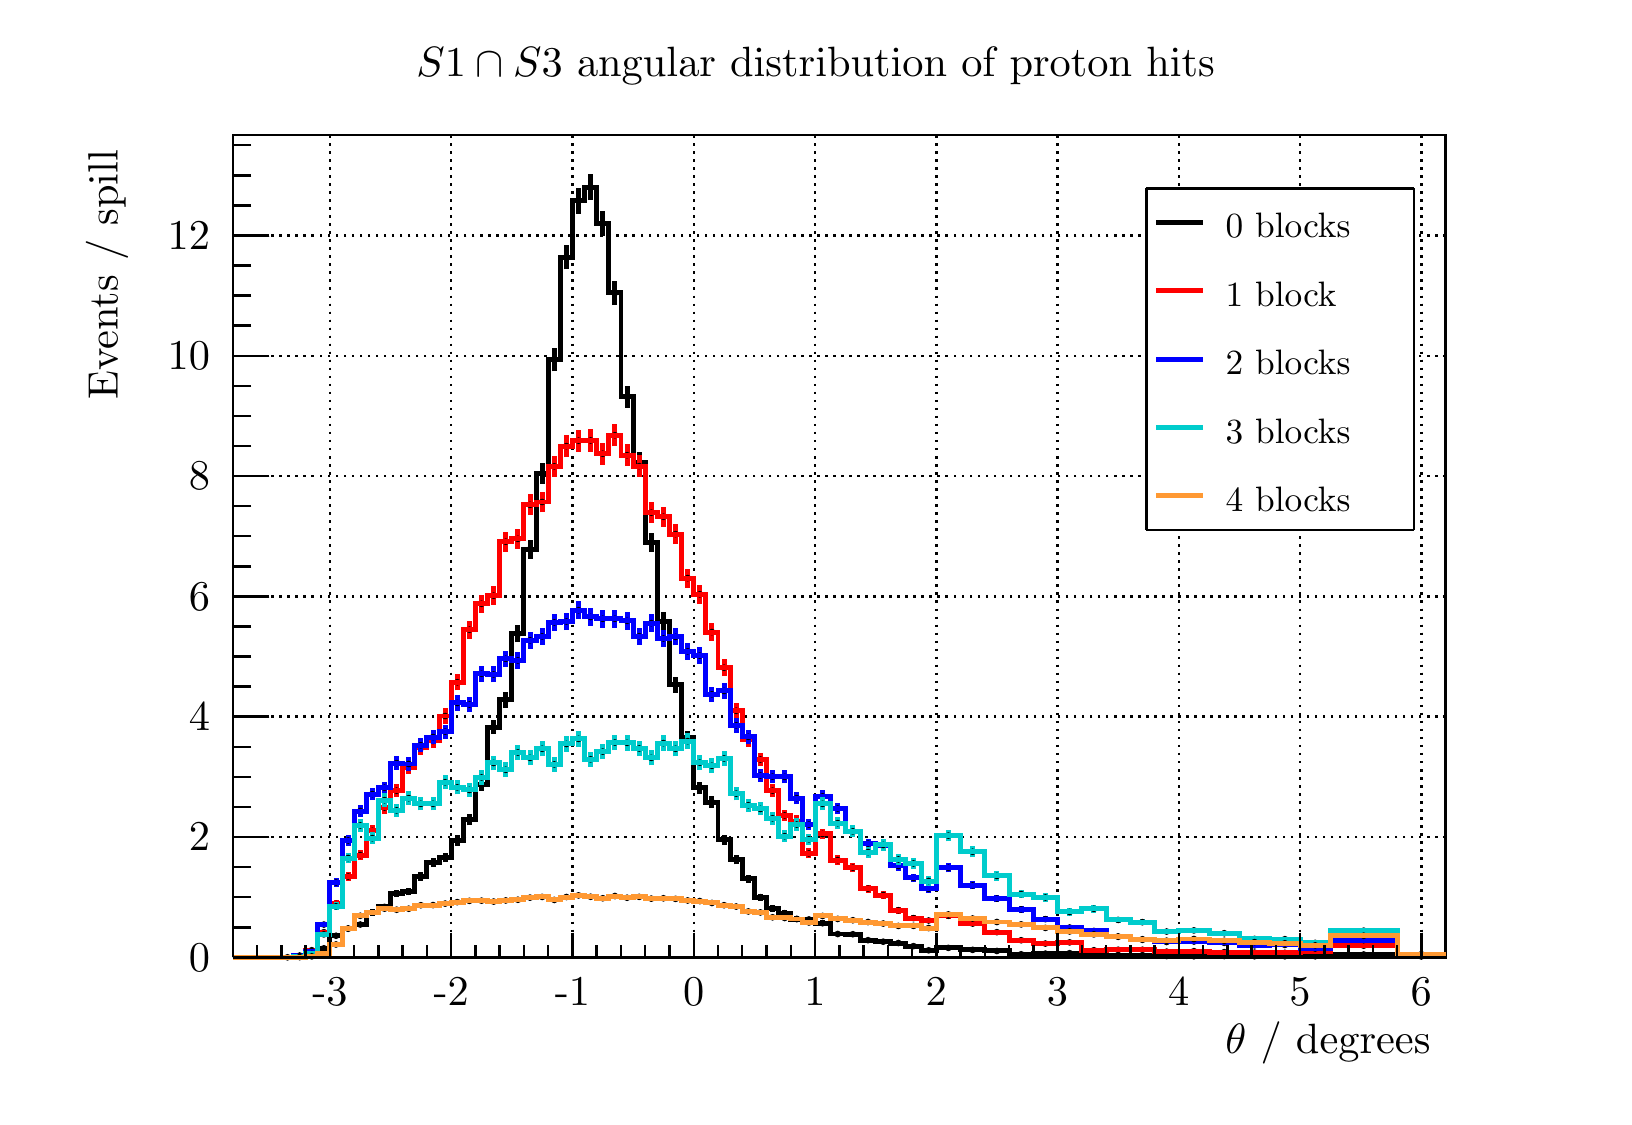
\begin{tikzpicture}
\pgfdeclareplotmark{cross} {
\pgfpathmoveto{\pgfpoint{-0.3\pgfplotmarksize}{\pgfplotmarksize}}
\pgfpathlineto{\pgfpoint{+0.3\pgfplotmarksize}{\pgfplotmarksize}}
\pgfpathlineto{\pgfpoint{+0.3\pgfplotmarksize}{0.3\pgfplotmarksize}}
\pgfpathlineto{\pgfpoint{+1\pgfplotmarksize}{0.3\pgfplotmarksize}}
\pgfpathlineto{\pgfpoint{+1\pgfplotmarksize}{-0.3\pgfplotmarksize}}
\pgfpathlineto{\pgfpoint{+0.3\pgfplotmarksize}{-0.3\pgfplotmarksize}}
\pgfpathlineto{\pgfpoint{+0.3\pgfplotmarksize}{-1.\pgfplotmarksize}}
\pgfpathlineto{\pgfpoint{-0.3\pgfplotmarksize}{-1.\pgfplotmarksize}}
\pgfpathlineto{\pgfpoint{-0.3\pgfplotmarksize}{-0.3\pgfplotmarksize}}
\pgfpathlineto{\pgfpoint{-1.\pgfplotmarksize}{-0.3\pgfplotmarksize}}
\pgfpathlineto{\pgfpoint{-1.\pgfplotmarksize}{0.3\pgfplotmarksize}}
\pgfpathlineto{\pgfpoint{-0.3\pgfplotmarksize}{0.3\pgfplotmarksize}}
\pgfpathclose
\pgfusepathqstroke
}
\pgfdeclareplotmark{cross*} {
\pgfpathmoveto{\pgfpoint{-0.3\pgfplotmarksize}{\pgfplotmarksize}}
\pgfpathlineto{\pgfpoint{+0.3\pgfplotmarksize}{\pgfplotmarksize}}
\pgfpathlineto{\pgfpoint{+0.3\pgfplotmarksize}{0.3\pgfplotmarksize}}
\pgfpathlineto{\pgfpoint{+1\pgfplotmarksize}{0.3\pgfplotmarksize}}
\pgfpathlineto{\pgfpoint{+1\pgfplotmarksize}{-0.3\pgfplotmarksize}}
\pgfpathlineto{\pgfpoint{+0.3\pgfplotmarksize}{-0.3\pgfplotmarksize}}
\pgfpathlineto{\pgfpoint{+0.3\pgfplotmarksize}{-1.\pgfplotmarksize}}
\pgfpathlineto{\pgfpoint{-0.3\pgfplotmarksize}{-1.\pgfplotmarksize}}
\pgfpathlineto{\pgfpoint{-0.3\pgfplotmarksize}{-0.3\pgfplotmarksize}}
\pgfpathlineto{\pgfpoint{-1.\pgfplotmarksize}{-0.3\pgfplotmarksize}}
\pgfpathlineto{\pgfpoint{-1.\pgfplotmarksize}{0.3\pgfplotmarksize}}
\pgfpathlineto{\pgfpoint{-0.3\pgfplotmarksize}{0.3\pgfplotmarksize}}
\pgfpathclose
\pgfusepathqfillstroke
}
\pgfdeclareplotmark{newstar} {
\pgfpathmoveto{\pgfqpoint{0pt}{\pgfplotmarksize}}
\pgfpathlineto{\pgfqpointpolar{44}{0.5\pgfplotmarksize}}
\pgfpathlineto{\pgfqpointpolar{18}{\pgfplotmarksize}}
\pgfpathlineto{\pgfqpointpolar{-20}{0.5\pgfplotmarksize}}
\pgfpathlineto{\pgfqpointpolar{-54}{\pgfplotmarksize}}
\pgfpathlineto{\pgfqpointpolar{-90}{0.5\pgfplotmarksize}}
\pgfpathlineto{\pgfqpointpolar{234}{\pgfplotmarksize}}
\pgfpathlineto{\pgfqpointpolar{198}{0.5\pgfplotmarksize}}
\pgfpathlineto{\pgfqpointpolar{162}{\pgfplotmarksize}}
\pgfpathlineto{\pgfqpointpolar{134}{0.5\pgfplotmarksize}}
\pgfpathclose
\pgfusepathqstroke
}
\pgfdeclareplotmark{newstar*} {
\pgfpathmoveto{\pgfqpoint{0pt}{\pgfplotmarksize}}
\pgfpathlineto{\pgfqpointpolar{44}{0.5\pgfplotmarksize}}
\pgfpathlineto{\pgfqpointpolar{18}{\pgfplotmarksize}}
\pgfpathlineto{\pgfqpointpolar{-20}{0.5\pgfplotmarksize}}
\pgfpathlineto{\pgfqpointpolar{-54}{\pgfplotmarksize}}
\pgfpathlineto{\pgfqpointpolar{-90}{0.5\pgfplotmarksize}}
\pgfpathlineto{\pgfqpointpolar{234}{\pgfplotmarksize}}
\pgfpathlineto{\pgfqpointpolar{198}{0.5\pgfplotmarksize}}
\pgfpathlineto{\pgfqpointpolar{162}{\pgfplotmarksize}}
\pgfpathlineto{\pgfqpointpolar{134}{0.5\pgfplotmarksize}}
\pgfpathclose
\pgfusepathqfillstroke
}
\definecolor{c}{rgb}{1,1,1};
\draw [color=c, fill=c] (0,0) rectangle (20,13.5632);
\draw [color=c, fill=c] (2.6,1.76322) rectangle (18,12.2069);
\definecolor{c}{rgb}{0,0,0};
\draw [c,line width=0.9] (2.6,1.76322) -- (2.6,12.2069) -- (18,12.2069) -- (18,1.76322) -- (2.6,1.76322);
\definecolor{c}{rgb}{1,1,1};
\draw [color=c, fill=c] (2.6,1.76322) rectangle (18,12.2069);
\definecolor{c}{rgb}{0,0,0};
\draw [c,line width=0.9] (2.6,1.76322) -- (2.6,12.2069) -- (18,12.2069) -- (18,1.76322) -- (2.6,1.76322);
\draw [c,line width=0.9] (2.6,1.76322) -- (18,1.76322);
\draw [c,dotted,line width=0.9] (3.832,12.2069) -- (3.832,1.76322);
\draw [c,dotted,line width=0.9] (5.372,12.2069) -- (5.372,1.76322);
\draw [c,dotted,line width=0.9] (6.912,12.2069) -- (6.912,1.76322);
\draw [c,dotted,line width=0.9] (8.452,12.2069) -- (8.452,1.76322);
\draw [c,dotted,line width=0.9] (9.992,12.2069) -- (9.992,1.76322);
\draw [c,dotted,line width=0.9] (11.532,12.2069) -- (11.532,1.76322);
\draw [c,dotted,line width=0.9] (13.072,12.2069) -- (13.072,1.76322);
\draw [c,dotted,line width=0.9] (14.612,12.2069) -- (14.612,1.76322);
\draw [c,dotted,line width=0.9] (16.152,12.2069) -- (16.152,1.76322);
\draw [c,dotted,line width=0.9] (17.692,12.2069) -- (17.692,1.76322);
\draw [c,dotted,line width=0.9] (3.832,12.2069) -- (3.832,1.76322);
\draw [c,dotted,line width=0.9] (17.692,12.2069) -- (17.692,1.76322);
\draw [c,line width=0.9] (2.6,1.76322) -- (2.6,12.2069);
\draw [c,dotted,line width=0.9] (18,1.76322) -- (2.6,1.76322);
\draw [c,dotted,line width=0.9] (18,3.29122) -- (2.6,3.29122);
\draw [c,dotted,line width=0.9] (18,4.81923) -- (2.6,4.81923);
\draw [c,dotted,line width=0.9] (18,6.34723) -- (2.6,6.34723);
\draw [c,dotted,line width=0.9] (18,7.87524) -- (2.6,7.87524);
\draw [c,dotted,line width=0.9] (18,9.40325) -- (2.6,9.40325);
\draw [c,dotted,line width=0.9] (18,10.9313) -- (2.6,10.9313);
\draw [c,dotted,line width=0.9] (18,10.9313) -- (2.6,10.9313);
\definecolor{c}{rgb}{0,0,0.6};
\draw [c,line width=0.9] (2.6,1.76322) -- (2.754,1.76322) -- (2.754,1.76322) -- (2.908,1.76322) -- (2.908,1.76322) -- (3.062,1.76322) -- (3.062,1.76322) -- (3.216,1.76322) -- (3.216,1.76322) -- (3.37,1.76322) -- (3.37,1.76322) -- (3.524,1.76322) --
 (3.524,1.76322) -- (3.678,1.76322) -- (3.678,1.76322) -- (3.832,1.76322) -- (3.832,1.76322) -- (3.986,1.76322) -- (3.986,1.76322) -- (4.14,1.76322) -- (4.14,1.76322) -- (4.294,1.76322) -- (4.294,1.76322) -- (4.448,1.76322) -- (4.448,1.76322) --
 (4.602,1.76322) -- (4.602,1.76322) -- (4.756,1.76322) -- (4.756,1.76322) -- (4.91,1.76322) -- (4.91,1.76322) -- (5.064,1.76322) -- (5.064,1.76322) -- (5.218,1.76322) -- (5.218,1.76322) -- (5.372,1.76322) -- (5.372,1.76322) -- (5.526,1.76322) --
 (5.526,1.76322) -- (5.68,1.76322) -- (5.68,1.76322) -- (5.834,1.76322) -- (5.834,1.76322) -- (5.988,1.76322) -- (5.988,1.76322) -- (6.142,1.76322) -- (6.142,1.76322) -- (6.296,1.76322) -- (6.296,1.76322) -- (6.45,1.76322) -- (6.45,1.76322) --
 (6.604,1.76322) -- (6.604,1.76322) -- (6.758,1.76322) -- (6.758,1.76322) -- (6.912,1.76322) -- (6.912,1.76322) -- (7.066,1.76322) -- (7.066,1.76322) -- (7.22,1.76322) -- (7.22,1.76322) -- (7.374,1.76322) -- (7.374,1.76322) -- (7.528,1.76322) --
 (7.528,1.76322) -- (7.682,1.76322) -- (7.682,1.76322) -- (7.836,1.76322) -- (7.836,1.76322) -- (7.99,1.76322) -- (7.99,1.76322) -- (8.144,1.76322) -- (8.144,1.76322) -- (8.298,1.76322) -- (8.298,1.76322) -- (8.452,1.76322) -- (8.452,1.76322) --
 (8.606,1.76322) -- (8.606,1.76322) -- (8.76,1.76322) -- (8.76,1.76322) -- (8.914,1.76322) -- (8.914,1.76322) -- (9.068,1.76322) -- (9.068,1.76322) -- (9.222,1.76322) -- (9.222,1.76322) -- (9.376,1.76322) -- (9.376,1.76322) -- (9.53,1.76322) --
 (9.53,1.76322) -- (9.684,1.76322) -- (9.684,1.76322) -- (9.838,1.76322) -- (9.838,1.76322) -- (9.992,1.76322) -- (9.992,1.76322) -- (10.1845,1.76322) -- (10.1845,1.76322) -- (10.377,1.76322) -- (10.377,1.76322) -- (10.5695,1.76322) --
 (10.5695,1.76322) -- (10.762,1.76322) -- (10.762,1.76322) -- (10.9545,1.76322) -- (10.9545,1.76322) -- (11.147,1.76322) -- (11.147,1.76322) -- (11.3395,1.76322) -- (11.3395,1.76322) -- (11.532,1.76322) -- (11.532,1.76322) -- (11.84,1.76322) --
 (11.84,1.76322) -- (12.148,1.76322) -- (12.148,1.76322) -- (12.456,1.76322) -- (12.456,1.76322) -- (12.764,1.76322) -- (12.764,1.76322) -- (13.072,1.76322) -- (13.072,1.76322) -- (13.38,1.76322) -- (13.38,1.76322) -- (13.688,1.76322) --
 (13.688,1.76322) -- (13.996,1.76322) -- (13.996,1.76322) -- (14.304,1.76322) -- (14.304,1.76322) -- (14.612,1.76322) -- (14.612,1.76322) -- (14.997,1.76322) -- (14.997,1.76322) -- (15.382,1.76322) -- (15.382,1.76322) -- (15.767,1.76322) --
 (15.767,1.76322) -- (16.152,1.76322) -- (16.152,1.76322) -- (16.537,1.76322) -- (16.537,1.76322) -- (17.384,1.76322) -- (17.384,1.76322) -- (18,1.76322);
\definecolor{c}{rgb}{0,0,0};
\draw [c,line width=0.9] (2.6,1.76322) -- (18,1.76322);
\draw [anchor= east] (18,0.678161) node[scale=1.5317, color=c, rotate=0]{$ \theta$ / degrees};
\draw [c,line width=0.9] (3.832,2.07653) -- (3.832,1.76322);
\draw [c,line width=0.9] (4.14,1.91987) -- (4.14,1.76322);
\draw [c,line width=0.9] (4.448,1.91987) -- (4.448,1.76322);
\draw [c,line width=0.9] (4.756,1.91987) -- (4.756,1.76322);
\draw [c,line width=0.9] (5.064,1.91987) -- (5.064,1.76322);
\draw [c,line width=0.9] (5.372,2.07653) -- (5.372,1.76322);
\draw [c,line width=0.9] (5.68,1.91987) -- (5.68,1.76322);
\draw [c,line width=0.9] (5.988,1.91987) -- (5.988,1.76322);
\draw [c,line width=0.9] (6.296,1.91987) -- (6.296,1.76322);
\draw [c,line width=0.9] (6.604,1.91987) -- (6.604,1.76322);
\draw [c,line width=0.9] (6.912,2.07653) -- (6.912,1.76322);
\draw [c,line width=0.9] (7.22,1.91987) -- (7.22,1.76322);
\draw [c,line width=0.9] (7.528,1.91987) -- (7.528,1.76322);
\draw [c,line width=0.9] (7.836,1.91987) -- (7.836,1.76322);
\draw [c,line width=0.9] (8.144,1.91987) -- (8.144,1.76322);
\draw [c,line width=0.9] (8.452,2.07653) -- (8.452,1.76322);
\draw [c,line width=0.9] (8.76,1.91987) -- (8.76,1.76322);
\draw [c,line width=0.9] (9.068,1.91987) -- (9.068,1.76322);
\draw [c,line width=0.9] (9.376,1.91987) -- (9.376,1.76322);
\draw [c,line width=0.9] (9.684,1.91987) -- (9.684,1.76322);
\draw [c,line width=0.9] (9.992,2.07653) -- (9.992,1.76322);
\draw [c,line width=0.9] (10.3,1.91987) -- (10.3,1.76322);
\draw [c,line width=0.9] (10.608,1.91987) -- (10.608,1.76322);
\draw [c,line width=0.9] (10.916,1.91987) -- (10.916,1.76322);
\draw [c,line width=0.9] (11.224,1.91987) -- (11.224,1.76322);
\draw [c,line width=0.9] (11.532,2.07653) -- (11.532,1.76322);
\draw [c,line width=0.9] (11.84,1.91987) -- (11.84,1.76322);
\draw [c,line width=0.9] (12.148,1.91987) -- (12.148,1.76322);
\draw [c,line width=0.9] (12.456,1.91987) -- (12.456,1.76322);
\draw [c,line width=0.9] (12.764,1.91987) -- (12.764,1.76322);
\draw [c,line width=0.9] (13.072,2.07653) -- (13.072,1.76322);
\draw [c,line width=0.9] (13.38,1.91987) -- (13.38,1.76322);
\draw [c,line width=0.9] (13.688,1.91987) -- (13.688,1.76322);
\draw [c,line width=0.9] (13.996,1.91987) -- (13.996,1.76322);
\draw [c,line width=0.9] (14.304,1.91987) -- (14.304,1.76322);
\draw [c,line width=0.9] (14.612,2.07653) -- (14.612,1.76322);
\draw [c,line width=0.9] (14.92,1.91987) -- (14.92,1.76322);
\draw [c,line width=0.9] (15.228,1.91987) -- (15.228,1.76322);
\draw [c,line width=0.9] (15.536,1.91987) -- (15.536,1.76322);
\draw [c,line width=0.9] (15.844,1.91987) -- (15.844,1.76322);
\draw [c,line width=0.9] (16.152,2.07653) -- (16.152,1.76322);
\draw [c,line width=0.9] (16.46,1.91987) -- (16.46,1.76322);
\draw [c,line width=0.9] (16.768,1.91987) -- (16.768,1.76322);
\draw [c,line width=0.9] (17.076,1.91987) -- (17.076,1.76322);
\draw [c,line width=0.9] (17.384,1.91987) -- (17.384,1.76322);
\draw [c,line width=0.9] (17.692,2.07653) -- (17.692,1.76322);
\draw [c,line width=0.9] (3.832,2.07653) -- (3.832,1.76322);
\draw [c,line width=0.9] (3.524,1.91987) -- (3.524,1.76322);
\draw [c,line width=0.9] (3.216,1.91987) -- (3.216,1.76322);
\draw [c,line width=0.9] (2.908,1.91987) -- (2.908,1.76322);
\draw [c,line width=0.9] (17.692,2.07653) -- (17.692,1.76322);
\draw [anchor=base] (3.832,1.15287) node[scale=1.5317, color=c, rotate=0]{-3};
\draw [anchor=base] (5.372,1.15287) node[scale=1.5317, color=c, rotate=0]{-2};
\draw [anchor=base] (6.912,1.15287) node[scale=1.5317, color=c, rotate=0]{-1};
\draw [anchor=base] (8.452,1.15287) node[scale=1.5317, color=c, rotate=0]{0};
\draw [anchor=base] (9.992,1.15287) node[scale=1.5317, color=c, rotate=0]{1};
\draw [anchor=base] (11.532,1.15287) node[scale=1.5317, color=c, rotate=0]{2};
\draw [anchor=base] (13.072,1.15287) node[scale=1.5317, color=c, rotate=0]{3};
\draw [anchor=base] (14.612,1.15287) node[scale=1.5317, color=c, rotate=0]{4};
\draw [anchor=base] (16.152,1.15287) node[scale=1.5317, color=c, rotate=0]{5};
\draw [anchor=base] (17.692,1.15287) node[scale=1.5317, color=c, rotate=0]{6};
\draw [c,line width=0.9] (2.6,1.76322) -- (2.6,12.2069);
\draw [anchor= east] (1,12.2069) node[scale=1.5317, color=c, rotate=90]{ Events / spill};
\draw [c,line width=0.9] (3.062,1.76322) -- (2.6,1.76322);
\draw [c,line width=0.9] (2.831,2.14522) -- (2.6,2.14522);
\draw [c,line width=0.9] (2.831,2.52722) -- (2.6,2.52722);
\draw [c,line width=0.9] (2.831,2.90922) -- (2.6,2.90922);
\draw [c,line width=0.9] (3.062,3.29122) -- (2.6,3.29122);
\draw [c,line width=0.9] (2.831,3.67323) -- (2.6,3.67323);
\draw [c,line width=0.9] (2.831,4.05523) -- (2.6,4.05523);
\draw [c,line width=0.9] (2.831,4.43723) -- (2.6,4.43723);
\draw [c,line width=0.9] (3.062,4.81923) -- (2.6,4.81923);
\draw [c,line width=0.9] (2.831,5.20123) -- (2.6,5.20123);
\draw [c,line width=0.9] (2.831,5.58323) -- (2.6,5.58323);
\draw [c,line width=0.9] (2.831,5.96523) -- (2.6,5.96523);
\draw [c,line width=0.9] (3.062,6.34723) -- (2.6,6.34723);
\draw [c,line width=0.9] (2.831,6.72924) -- (2.6,6.72924);
\draw [c,line width=0.9] (2.831,7.11124) -- (2.6,7.11124);
\draw [c,line width=0.9] (2.831,7.49324) -- (2.6,7.49324);
\draw [c,line width=0.9] (3.062,7.87524) -- (2.6,7.87524);
\draw [c,line width=0.9] (2.831,8.25724) -- (2.6,8.25724);
\draw [c,line width=0.9] (2.831,8.63924) -- (2.6,8.63924);
\draw [c,line width=0.9] (2.831,9.02124) -- (2.6,9.02124);
\draw [c,line width=0.9] (3.062,9.40325) -- (2.6,9.40325);
\draw [c,line width=0.9] (2.831,9.78525) -- (2.6,9.78525);
\draw [c,line width=0.9] (2.831,10.1672) -- (2.6,10.1672);
\draw [c,line width=0.9] (2.831,10.5492) -- (2.6,10.5492);
\draw [c,line width=0.9] (3.062,10.9313) -- (2.6,10.9313);
\draw [c,line width=0.9] (3.062,10.9313) -- (2.6,10.9313);
\draw [c,line width=0.9] (2.831,11.3133) -- (2.6,11.3133);
\draw [c,line width=0.9] (2.831,11.6953) -- (2.6,11.6953);
\draw [c,line width=0.9] (2.831,12.0773) -- (2.6,12.0773);
\draw [anchor= east] (2.5,1.76322) node[scale=1.5317, color=c, rotate=0]{0};
\draw [anchor= east] (2.5,3.29122) node[scale=1.5317, color=c, rotate=0]{2};
\draw [anchor= east] (2.5,4.81923) node[scale=1.5317, color=c, rotate=0]{4};
\draw [anchor= east] (2.5,6.34723) node[scale=1.5317, color=c, rotate=0]{6};
\draw [anchor= east] (2.5,7.87524) node[scale=1.5317, color=c, rotate=0]{8};
\draw [anchor= east] (2.5,9.40325) node[scale=1.5317, color=c, rotate=0]{10};
\draw [anchor= east] (2.5,10.9313) node[scale=1.5317, color=c, rotate=0]{12};
\draw [c,line width=1.8] (3.447,1.76882) -- (3.447,1.77441);
\draw [c,line width=1.8] (3.447,1.77441) -- (3.447,1.78001);
\foreach \P in {(3.447,1.77441)}{\draw[mark options={color=c,fill=c},mark size=2.402402pt,mark=*,mark size=1pt] plot coordinates {\P};}
\draw [c,line width=1.8] (3.601,1.78711) -- (3.601,1.7968);
\draw [c,line width=1.8] (3.601,1.7968) -- (3.601,1.8065);
\foreach \P in {(3.601,1.7968)}{\draw[mark options={color=c,fill=c},mark size=2.402402pt,mark=*,mark size=1pt] plot coordinates {\P};}
\draw [c,line width=1.8] (3.755,1.86004) -- (3.755,1.87796);
\draw [c,line width=1.8] (3.755,1.87796) -- (3.755,1.89588);
\foreach \P in {(3.755,1.87796)}{\draw[mark options={color=c,fill=c},mark size=2.402402pt,mark=*,mark size=1pt] plot coordinates {\P};}
\draw [c,line width=1.8] (3.909,2.00977) -- (3.909,2.03748);
\draw [c,line width=1.8] (3.909,2.03748) -- (3.909,2.06518);
\foreach \P in {(3.909,2.03748)}{\draw[mark options={color=c,fill=c},mark size=2.402402pt,mark=*,mark size=1pt] plot coordinates {\P};}
\draw [c,line width=1.8] (4.063,2.09512) -- (4.063,2.12703);
\draw [c,line width=1.8] (4.063,2.12703) -- (4.063,2.15894);
\foreach \P in {(4.063,2.12703)}{\draw[mark options={color=c,fill=c},mark size=2.402402pt,mark=*,mark size=1pt] plot coordinates {\P};}
\draw [c,line width=1.8] (4.217,2.14604) -- (4.217,2.1802);
\draw [c,line width=1.8] (4.217,2.1802) -- (4.217,2.21436);
\foreach \P in {(4.217,2.1802)}{\draw[mark options={color=c,fill=c},mark size=2.402402pt,mark=*,mark size=1pt] plot coordinates {\P};}
\draw [c,line width=1.8] (4.371,2.29145) -- (4.371,2.33132);
\draw [c,line width=1.8] (4.371,2.33132) -- (4.371,2.3712);
\foreach \P in {(4.371,2.33132)}{\draw[mark options={color=c,fill=c},mark size=2.402402pt,mark=*,mark size=1pt] plot coordinates {\P};}
\draw [c,line width=1.8] (4.525,2.36174) -- (4.525,2.40409);
\draw [c,line width=1.8] (4.525,2.40409) -- (4.525,2.44643);
\foreach \P in {(4.525,2.40409)}{\draw[mark options={color=c,fill=c},mark size=2.402402pt,mark=*,mark size=1pt] plot coordinates {\P};}
\draw [c,line width=1.8] (4.679,2.52714) -- (4.679,2.5748);
\draw [c,line width=1.8] (4.679,2.5748) -- (4.679,2.62245);
\foreach \P in {(4.679,2.5748)}{\draw[mark options={color=c,fill=c},mark size=2.402402pt,mark=*,mark size=1pt] plot coordinates {\P};}
\draw [c,line width=1.8] (4.833,2.54887) -- (4.833,2.59718);
\draw [c,line width=1.8] (4.833,2.59718) -- (4.833,2.64549);
\foreach \P in {(4.833,2.59718)}{\draw[mark options={color=c,fill=c},mark size=2.402402pt,mark=*,mark size=1pt] plot coordinates {\P};}
\draw [c,line width=1.8] (4.987,2.73395) -- (4.987,2.78749);
\draw [c,line width=1.8] (4.987,2.78749) -- (4.987,2.84103);
\foreach \P in {(4.987,2.78749)}{\draw[mark options={color=c,fill=c},mark size=2.402402pt,mark=*,mark size=1pt] plot coordinates {\P};}
\draw [c,line width=1.8] (5.141,2.90856) -- (5.141,2.96659);
\draw [c,line width=1.8] (5.141,2.96659) -- (5.141,3.02462);
\foreach \P in {(5.141,2.96659)}{\draw[mark options={color=c,fill=c},mark size=2.402402pt,mark=*,mark size=1pt] plot coordinates {\P};}
\draw [c,line width=1.8] (5.295,2.97413) -- (5.295,3.03376);
\draw [c,line width=1.8] (5.295,3.03376) -- (5.295,3.09339);
\foreach \P in {(5.295,3.03376)}{\draw[mark options={color=c,fill=c},mark size=2.402402pt,mark=*,mark size=1pt] plot coordinates {\P};}
\draw [c,line width=1.8] (5.449,3.18202) -- (5.449,3.24645);
\draw [c,line width=1.8] (5.449,3.24645) -- (5.449,3.31087);
\foreach \P in {(5.449,3.24645)}{\draw[mark options={color=c,fill=c},mark size=2.402402pt,mark=*,mark size=1pt] plot coordinates {\P};}
\draw [c,line width=1.8] (5.603,3.4396) -- (5.603,3.50951);
\draw [c,line width=1.8] (5.603,3.50951) -- (5.603,3.57942);
\foreach \P in {(5.603,3.50951)}{\draw[mark options={color=c,fill=c},mark size=2.402402pt,mark=*,mark size=1pt] plot coordinates {\P};}
\draw [c,line width=1.8] (5.757,3.87617) -- (5.757,3.95448);
\draw [c,line width=1.8] (5.757,3.95448) -- (5.757,4.03279);
\foreach \P in {(5.757,3.95448)}{\draw[mark options={color=c,fill=c},mark size=2.402402pt,mark=*,mark size=1pt] plot coordinates {\P};}
\draw [c,line width=1.8] (5.911,4.59723) -- (5.911,4.6877);
\draw [c,line width=1.8] (5.911,4.6877) -- (5.911,4.77816);
\foreach \P in {(5.911,4.6877)}{\draw[mark options={color=c,fill=c},mark size=2.402402pt,mark=*,mark size=1pt] plot coordinates {\P};}
\draw [c,line width=1.8] (6.065,4.93628) -- (6.065,5.03192);
\draw [c,line width=1.8] (6.065,5.03192) -- (6.065,5.12756);
\foreach \P in {(6.065,5.03192)}{\draw[mark options={color=c,fill=c},mark size=2.402402pt,mark=*,mark size=1pt] plot coordinates {\P};}
\draw [c,line width=1.8] (6.219,5.76426) -- (6.219,5.87148);
\draw [c,line width=1.8] (6.219,5.87148) -- (6.219,5.97871);
\foreach \P in {(6.219,5.87148)}{\draw[mark options={color=c,fill=c},mark size=2.402402pt,mark=*,mark size=1pt] plot coordinates {\P};}
\draw [c,line width=1.8] (6.373,6.82569) -- (6.373,6.94612);
\draw [c,line width=1.8] (6.373,6.94612) -- (6.373,7.06656);
\foreach \P in {(6.373,6.94612)}{\draw[mark options={color=c,fill=c},mark size=2.402402pt,mark=*,mark size=1pt] plot coordinates {\P};}
\draw [c,line width=1.8] (6.527,7.77491) -- (6.527,7.90602);
\draw [c,line width=1.8] (6.527,7.90602) -- (6.527,8.03714);
\foreach \P in {(6.527,7.90602)}{\draw[mark options={color=c,fill=c},mark size=2.402402pt,mark=*,mark size=1pt] plot coordinates {\P};}
\draw [c,line width=1.8] (6.681,9.20436) -- (6.681,9.35007);
\draw [c,line width=1.8] (6.681,9.35007) -- (6.681,9.49579);
\foreach \P in {(6.681,9.35007)}{\draw[mark options={color=c,fill=c},mark size=2.402402pt,mark=*,mark size=1pt] plot coordinates {\P};}
\draw [c,line width=1.8] (6.835,10.4992) -- (6.835,10.657);
\draw [c,line width=1.8] (6.835,10.657) -- (6.835,10.8148);
\foreach \P in {(6.835,10.657)}{\draw[mark options={color=c,fill=c},mark size=2.402402pt,mark=*,mark size=1pt] plot coordinates {\P};}
\draw [c,line width=1.8] (6.989,11.2067) -- (6.989,11.3706);
\draw [c,line width=1.8] (6.989,11.3706) -- (6.989,11.5346);
\foreach \P in {(6.989,11.3706)}{\draw[mark options={color=c,fill=c},mark size=2.402402pt,mark=*,mark size=1pt] plot coordinates {\P};}
\draw [c,line width=1.8] (7.143,11.3787) -- (7.143,11.5441);
\draw [c,line width=1.8] (7.143,11.5441) -- (7.143,11.7096);
\foreach \P in {(7.143,11.5441)}{\draw[mark options={color=c,fill=c},mark size=2.402402pt,mark=*,mark size=1pt] plot coordinates {\P};}
\draw [c,line width=1.8] (7.297,10.9181) -- (7.297,11.0796);
\draw [c,line width=1.8] (7.297,11.0796) -- (7.297,11.241);
\foreach \P in {(7.297,11.0796)}{\draw[mark options={color=c,fill=c},mark size=2.402402pt,mark=*,mark size=1pt] plot coordinates {\P};}
\draw [c,line width=1.8] (7.451,10.0472) -- (7.451,10.2008);
\draw [c,line width=1.8] (7.451,10.2008) -- (7.451,10.3545);
\foreach \P in {(7.451,10.2008)}{\draw[mark options={color=c,fill=c},mark size=2.402402pt,mark=*,mark size=1pt] plot coordinates {\P};}
\draw [c,line width=1.8] (7.605,8.74156) -- (7.605,8.88272);
\draw [c,line width=1.8] (7.605,8.88272) -- (7.605,9.02387);
\foreach \P in {(7.605,8.88272)}{\draw[mark options={color=c,fill=c},mark size=2.402402pt,mark=*,mark size=1pt] plot coordinates {\P};}
\draw [c,line width=1.8] (7.759,7.91335) -- (7.759,8.04595);
\draw [c,line width=1.8] (7.759,8.04595) -- (7.759,8.17855);
\foreach \P in {(7.759,8.04595)}{\draw[mark options={color=c,fill=c},mark size=2.402402pt,mark=*,mark size=1pt] plot coordinates {\P};}
\draw [c,line width=1.8] (7.913,6.90867) -- (7.913,7.03008);
\draw [c,line width=1.8] (7.913,7.03008) -- (7.913,7.15149);
\foreach \P in {(7.913,7.03008)}{\draw[mark options={color=c,fill=c},mark size=2.402402pt,mark=*,mark size=1pt] plot coordinates {\P};}
\draw [c,line width=1.8] (8.067,5.92448) -- (8.067,6.0338);
\draw [c,line width=1.8] (8.067,6.0338) -- (8.067,6.14312);
\foreach \P in {(8.067,6.0338)}{\draw[mark options={color=c,fill=c},mark size=2.402402pt,mark=*,mark size=1pt] plot coordinates {\P};}
\draw [c,line width=1.8] (8.221,5.12659) -- (8.221,5.22502);
\draw [c,line width=1.8] (8.221,5.22502) -- (8.221,5.32345);
\foreach \P in {(8.221,5.22502)}{\draw[mark options={color=c,fill=c},mark size=2.402402pt,mark=*,mark size=1pt] plot coordinates {\P};}
\draw [c,line width=1.8] (8.375,4.46225) -- (8.375,4.55057);
\draw [c,line width=1.8] (8.375,4.55057) -- (8.375,4.63889);
\foreach \P in {(8.375,4.55057)}{\draw[mark options={color=c,fill=c},mark size=2.402402pt,mark=*,mark size=1pt] plot coordinates {\P};}
\draw [c,line width=1.8] (8.529,3.83769) -- (8.529,3.9153);
\draw [c,line width=1.8] (8.529,3.9153) -- (8.529,3.99291);
\foreach \P in {(8.529,3.9153)}{\draw[mark options={color=c,fill=c},mark size=2.402402pt,mark=*,mark size=1pt] plot coordinates {\P};}
\draw [c,line width=1.8] (8.683,3.65914) -- (8.683,3.73339);
\draw [c,line width=1.8] (8.683,3.73339) -- (8.683,3.80765);
\foreach \P in {(8.683,3.73339)}{\draw[mark options={color=c,fill=c},mark size=2.402402pt,mark=*,mark size=1pt] plot coordinates {\P};}
\draw [c,line width=1.8] (8.837,3.19297) -- (8.837,3.25764);
\draw [c,line width=1.8] (8.837,3.25764) -- (8.837,3.32231);
\foreach \P in {(8.837,3.25764)}{\draw[mark options={color=c,fill=c},mark size=2.402402pt,mark=*,mark size=1pt] plot coordinates {\P};}
\draw [c,line width=1.8] (8.991,2.94407) -- (8.991,3.00297);
\draw [c,line width=1.8] (8.991,3.00297) -- (8.991,3.06188);
\foreach \P in {(8.991,3.00297)}{\draw[mark options={color=c,fill=c},mark size=2.402402pt,mark=*,mark size=1pt] plot coordinates {\P};}
\draw [c,line width=1.8] (9.145,2.70942) -- (9.145,2.7623);
\draw [c,line width=1.8] (9.145,2.7623) -- (9.145,2.81518);
\foreach \P in {(9.145,2.7623)}{\draw[mark options={color=c,fill=c},mark size=2.402402pt,mark=*,mark size=1pt] plot coordinates {\P};}
\draw [c,line width=1.8] (9.299,2.48098) -- (9.299,2.52722);
\draw [c,line width=1.8] (9.299,2.52722) -- (9.299,2.57346);
\foreach \P in {(9.299,2.52722)}{\draw[mark options={color=c,fill=c},mark size=2.402402pt,mark=*,mark size=1pt] plot coordinates {\P};}
\draw [c,line width=1.8] (9.453,2.34009) -- (9.453,2.3817);
\draw [c,line width=1.8] (9.453,2.3817) -- (9.453,2.4233);
\foreach \P in {(9.453,2.3817)}{\draw[mark options={color=c,fill=c},mark size=2.402402pt,mark=*,mark size=1pt] plot coordinates {\P};}
\draw [c,line width=1.8] (9.607,2.28335) -- (9.607,2.32293);
\draw [c,line width=1.8] (9.607,2.32293) -- (9.607,2.3625);
\foreach \P in {(9.607,2.32293)}{\draw[mark options={color=c,fill=c},mark size=2.402402pt,mark=*,mark size=1pt] plot coordinates {\P};}
\draw [c,line width=1.8] (9.761,2.21325) -- (9.761,2.25017);
\draw [c,line width=1.8] (9.761,2.25017) -- (9.761,2.28708);
\foreach \P in {(9.761,2.25017)}{\draw[mark options={color=c,fill=c},mark size=2.402402pt,mark=*,mark size=1pt] plot coordinates {\P};}
\draw [c,line width=1.8] (9.915,2.20787) -- (9.915,2.24457);
\draw [c,line width=1.8] (9.915,2.24457) -- (9.915,2.28127);
\foreach \P in {(9.915,2.24457)}{\draw[mark options={color=c,fill=c},mark size=2.402402pt,mark=*,mark size=1pt] plot coordinates {\P};}
\draw [c,line width=1.8] (10.0883,2.16215) -- (10.0883,2.19699);
\draw [c,line width=1.8] (10.0883,2.19699) -- (10.0883,2.23183);
\foreach \P in {(10.0883,2.19699)}{\draw[mark options={color=c,fill=c},mark size=2.402402pt,mark=*,mark size=1pt] plot coordinates {\P};}
\draw [c,line width=1.8] (10.2808,2.03105) -- (10.2808,2.05986);
\draw [c,line width=1.8] (10.2808,2.05986) -- (10.2808,2.08868);
\foreach \P in {(10.2808,2.05986)}{\draw[mark options={color=c,fill=c},mark size=2.402402pt,mark=*,mark size=1pt] plot coordinates {\P};}
\draw [c,line width=1.8] (10.4733,2.02839) -- (10.4733,2.05707);
\draw [c,line width=1.8] (10.4733,2.05707) -- (10.4733,2.08574);
\foreach \P in {(10.4733,2.05707)}{\draw[mark options={color=c,fill=c},mark size=2.402402pt,mark=*,mark size=1pt] plot coordinates {\P};}
\draw [c,line width=1.8] (10.6657,1.95679) -- (10.6657,1.9815);
\draw [c,line width=1.8] (10.6657,1.9815) -- (10.6657,2.00622);
\foreach \P in {(10.6657,1.9815)}{\draw[mark options={color=c,fill=c},mark size=2.402402pt,mark=*,mark size=1pt] plot coordinates {\P};}
\draw [c,line width=1.8] (10.8582,1.93833) -- (10.8582,1.96192);
\draw [c,line width=1.8] (10.8582,1.96192) -- (10.8582,1.9855);
\foreach \P in {(10.8582,1.96192)}{\draw[mark options={color=c,fill=c},mark size=2.402402pt,mark=*,mark size=1pt] plot coordinates {\P};}
\draw [c,line width=1.8] (11.0507,1.92256) -- (11.0507,1.94512);
\draw [c,line width=1.8] (11.0507,1.94512) -- (11.0507,1.96769);
\foreach \P in {(11.0507,1.94512)}{\draw[mark options={color=c,fill=c},mark size=2.402402pt,mark=*,mark size=1pt] plot coordinates {\P};}
\draw [c,line width=1.8] (11.2432,1.88596) -- (11.2432,1.90594);
\draw [c,line width=1.8] (11.2432,1.90594) -- (11.2432,1.92593);
\foreach \P in {(11.2432,1.90594)}{\draw[mark options={color=c,fill=c},mark size=2.402402pt,mark=*,mark size=1pt] plot coordinates {\P};}
\draw [c,line width=1.8] (11.4358,1.83694) -- (11.4358,1.85277);
\draw [c,line width=1.8] (11.4358,1.85277) -- (11.4358,1.8686);
\foreach \P in {(11.4358,1.85277)}{\draw[mark options={color=c,fill=c},mark size=2.402402pt,mark=*,mark size=1pt] plot coordinates {\P};}
\draw [c,line width=1.8] (11.686,1.8652) -- (11.686,1.88356);
\draw [c,line width=1.8] (11.686,1.88356) -- (11.686,1.90191);
\foreach \P in {(11.686,1.88356)}{\draw[mark options={color=c,fill=c},mark size=2.402402pt,mark=*,mark size=1pt] plot coordinates {\P};}
\draw [c,line width=1.8] (11.994,1.84205) -- (11.994,1.85837);
\draw [c,line width=1.8] (11.994,1.85837) -- (11.994,1.87469);
\foreach \P in {(11.994,1.85837)}{\draw[mark options={color=c,fill=c},mark size=2.402402pt,mark=*,mark size=1pt] plot coordinates {\P};}
\draw [c,line width=1.8] (12.302,1.82931) -- (12.302,1.84438);
\draw [c,line width=1.8] (12.302,1.84438) -- (12.302,1.85945);
\foreach \P in {(12.302,1.84438)}{\draw[mark options={color=c,fill=c},mark size=2.402402pt,mark=*,mark size=1pt] plot coordinates {\P};}
\draw [c,line width=1.8] (12.61,1.79193) -- (12.61,1.8024);
\draw [c,line width=1.8] (12.61,1.8024) -- (12.61,1.81287);
\foreach \P in {(12.61,1.8024)}{\draw[mark options={color=c,fill=c},mark size=2.402402pt,mark=*,mark size=1pt] plot coordinates {\P};}
\draw [c,line width=1.8] (12.918,1.79925) -- (12.918,1.81079);
\draw [c,line width=1.8] (12.918,1.81079) -- (12.918,1.82233);
\foreach \P in {(12.918,1.81079)}{\draw[mark options={color=c,fill=c},mark size=2.402402pt,mark=*,mark size=1pt] plot coordinates {\P};}
\draw [c,line width=1.8] (13.226,1.80419) -- (13.226,1.81639);
\draw [c,line width=1.8] (13.226,1.81639) -- (13.226,1.82859);
\foreach \P in {(13.226,1.81639)}{\draw[mark options={color=c,fill=c},mark size=2.402402pt,mark=*,mark size=1pt] plot coordinates {\P};}
\draw [c,line width=1.8] (13.534,1.78001) -- (13.534,1.78841);
\draw [c,line width=1.8] (13.534,1.78841) -- (13.534,1.7968);
\foreach \P in {(13.534,1.78841)}{\draw[mark options={color=c,fill=c},mark size=2.402402pt,mark=*,mark size=1pt] plot coordinates {\P};}
\draw [c,line width=1.8] (13.842,1.78235) -- (13.842,1.7912);
\draw [c,line width=1.8] (13.842,1.7912) -- (13.842,1.80005);
\foreach \P in {(13.842,1.7912)}{\draw[mark options={color=c,fill=c},mark size=2.402402pt,mark=*,mark size=1pt] plot coordinates {\P};}
\draw [c,line width=1.8] (14.15,1.77769) -- (14.15,1.78561);
\draw [c,line width=1.8] (14.15,1.78561) -- (14.15,1.79352);
\foreach \P in {(14.15,1.78561)}{\draw[mark options={color=c,fill=c},mark size=2.402402pt,mark=*,mark size=1pt] plot coordinates {\P};}
\draw [c,line width=1.8] (14.458,1.77315) -- (14.458,1.78001);
\draw [c,line width=1.8] (14.458,1.78001) -- (14.458,1.78686);
\foreach \P in {(14.458,1.78001)}{\draw[mark options={color=c,fill=c},mark size=2.402402pt,mark=*,mark size=1pt] plot coordinates {\P};}
\draw [c,line width=1.8] (14.8045,1.77095) -- (14.8045,1.77721);
\draw [c,line width=1.8] (14.8045,1.77721) -- (14.8045,1.78347);
\foreach \P in {(14.8045,1.77721)}{\draw[mark options={color=c,fill=c},mark size=2.402402pt,mark=*,mark size=1pt] plot coordinates {\P};}
\draw [c,line width=1.8] (15.1895,1.77315) -- (15.1895,1.78001);
\draw [c,line width=1.8] (15.1895,1.78001) -- (15.1895,1.78686);
\foreach \P in {(15.1895,1.78001)}{\draw[mark options={color=c,fill=c},mark size=2.402402pt,mark=*,mark size=1pt] plot coordinates {\P};}
\draw [c,line width=1.8] (15.5745,1.77095) -- (15.5745,1.77721);
\draw [c,line width=1.8] (15.5745,1.77721) -- (15.5745,1.78347);
\foreach \P in {(15.5745,1.77721)}{\draw[mark options={color=c,fill=c},mark size=2.402402pt,mark=*,mark size=1pt] plot coordinates {\P};}
\draw [c,line width=1.8] (15.9595,1.77095) -- (15.9595,1.77721);
\draw [c,line width=1.8] (15.9595,1.77721) -- (15.9595,1.78347);
\foreach \P in {(15.9595,1.77721)}{\draw[mark options={color=c,fill=c},mark size=2.402402pt,mark=*,mark size=1pt] plot coordinates {\P};}
\draw [c,line width=1.8] (16.3445,1.77095) -- (16.3445,1.77721);
\draw [c,line width=1.8] (16.3445,1.77721) -- (16.3445,1.78347);
\foreach \P in {(16.3445,1.77721)}{\draw[mark options={color=c,fill=c},mark size=2.402402pt,mark=*,mark size=1pt] plot coordinates {\P};}
\draw [c,line width=1.8] (16.9605,1.78951) -- (16.9605,1.7996);
\draw [c,line width=1.8] (16.9605,1.7996) -- (16.9605,1.80969);
\foreach \P in {(16.9605,1.7996)}{\draw[mark options={color=c,fill=c},mark size=2.402402pt,mark=*,mark size=1pt] plot coordinates {\P};}
\draw [c,line width=1.8] (17.692,1.76882) -- (17.692,1.77441);
\draw [c,line width=1.8] (17.692,1.77441) -- (17.692,1.78001);
\foreach \P in {(17.692,1.77441)}{\draw[mark options={color=c,fill=c},mark size=2.402402pt,mark=*,mark size=1pt] plot coordinates {\P};}
\draw [c,line width=1.8] (2.6,1.76322) -- (2.754,1.76322) -- (2.754,1.76322) -- (2.908,1.76322) -- (2.908,1.76322) -- (3.062,1.76322) -- (3.062,1.76322) -- (3.216,1.76322) -- (3.216,1.76322) -- (3.37,1.76322) -- (3.37,1.77441) -- (3.524,1.77441) --
 (3.524,1.7968) -- (3.678,1.7968) -- (3.678,1.87796) -- (3.832,1.87796) -- (3.832,2.03748) -- (3.986,2.03748) -- (3.986,2.12703) -- (4.14,2.12703) -- (4.14,2.1802) -- (4.294,2.1802) -- (4.294,2.33132) -- (4.448,2.33132) -- (4.448,2.40409) --
 (4.602,2.40409) -- (4.602,2.5748) -- (4.756,2.5748) -- (4.756,2.59718) -- (4.91,2.59718) -- (4.91,2.78749) -- (5.064,2.78749) -- (5.064,2.96659) -- (5.218,2.96659) -- (5.218,3.03376) -- (5.372,3.03376) -- (5.372,3.24645) -- (5.526,3.24645) --
 (5.526,3.50951) -- (5.68,3.50951) -- (5.68,3.95448) -- (5.834,3.95448) -- (5.834,4.6877) -- (5.988,4.6877) -- (5.988,5.03192) -- (6.142,5.03192) -- (6.142,5.87148) -- (6.296,5.87148) -- (6.296,6.94612) -- (6.45,6.94612) -- (6.45,7.90602) --
 (6.604,7.90602) -- (6.604,9.35007) -- (6.758,9.35007) -- (6.758,10.657) -- (6.912,10.657) -- (6.912,11.3706) -- (7.066,11.3706) -- (7.066,11.5441) -- (7.22,11.5441) -- (7.22,11.0796) -- (7.374,11.0796) -- (7.374,10.2008) -- (7.528,10.2008) --
 (7.528,8.88272) -- (7.682,8.88272) -- (7.682,8.04595) -- (7.836,8.04595) -- (7.836,7.03008) -- (7.99,7.03008) -- (7.99,6.0338) -- (8.144,6.0338) -- (8.144,5.22502) -- (8.298,5.22502) -- (8.298,4.55057) -- (8.452,4.55057) -- (8.452,3.9153) --
 (8.606,3.9153) -- (8.606,3.73339) -- (8.76,3.73339) -- (8.76,3.25764) -- (8.914,3.25764) -- (8.914,3.00297) -- (9.068,3.00297) -- (9.068,2.7623) -- (9.222,2.7623) -- (9.222,2.52722) -- (9.376,2.52722) -- (9.376,2.3817) -- (9.53,2.3817) --
 (9.53,2.32293) -- (9.684,2.32293) -- (9.684,2.25017) -- (9.838,2.25017) -- (9.838,2.24457) -- (9.992,2.24457) -- (9.992,2.19699) -- (10.1845,2.19699) -- (10.1845,2.05986) -- (10.377,2.05986) -- (10.377,2.05707) -- (10.5695,2.05707) --
 (10.5695,1.9815) -- (10.762,1.9815) -- (10.762,1.96192) -- (10.9545,1.96192) -- (10.9545,1.94512) -- (11.147,1.94512) -- (11.147,1.90594) -- (11.3395,1.90594) -- (11.3395,1.85277) -- (11.532,1.85277) -- (11.532,1.88356) -- (11.84,1.88356) --
 (11.84,1.85837) -- (12.148,1.85837) -- (12.148,1.84438) -- (12.456,1.84438) -- (12.456,1.8024) -- (12.764,1.8024) -- (12.764,1.81079) -- (13.072,1.81079) -- (13.072,1.81639) -- (13.38,1.81639) -- (13.38,1.78841) -- (13.688,1.78841) --
 (13.688,1.7912) -- (13.996,1.7912) -- (13.996,1.78561) -- (14.304,1.78561) -- (14.304,1.78001) -- (14.612,1.78001) -- (14.612,1.77721) -- (14.997,1.77721) -- (14.997,1.78001) -- (15.382,1.78001) -- (15.382,1.77721) -- (15.767,1.77721) --
 (15.767,1.77721) -- (16.152,1.77721) -- (16.152,1.77721) -- (16.537,1.77721) -- (16.537,1.7996) -- (17.384,1.7996) -- (17.384,1.77441) -- (18,1.77441);
\definecolor{c}{rgb}{1,0,0};
\draw [c,line width=1.8] (3.447,1.76499) -- (3.447,1.76926);
\draw [c,line width=1.8] (3.447,1.76926) -- (3.447,1.77353);
\definecolor{c}{rgb}{0,0,0};
\foreach \P in {(3.447,1.76926)}{\draw[mark options={color=c,fill=c},mark size=2.402402pt,mark=*,mark size=1pt] plot coordinates {\P};}
\definecolor{c}{rgb}{1,0,0};
\draw [c,line width=1.8] (3.601,1.83727) -- (3.601,1.85381);
\draw [c,line width=1.8] (3.601,1.85381) -- (3.601,1.87035);
\definecolor{c}{rgb}{0,0,0};
\foreach \P in {(3.601,1.85381)}{\draw[mark options={color=c,fill=c},mark size=2.402402pt,mark=*,mark size=1pt] plot coordinates {\P};}
\definecolor{c}{rgb}{1,0,0};
\draw [c,line width=1.8] (3.755,2.05222) -- (3.755,2.08331);
\draw [c,line width=1.8] (3.755,2.08331) -- (3.755,2.1144);
\definecolor{c}{rgb}{0,0,0};
\foreach \P in {(3.755,2.08331)}{\draw[mark options={color=c,fill=c},mark size=2.402402pt,mark=*,mark size=1pt] plot coordinates {\P};}
\definecolor{c}{rgb}{1,0,0};
\draw [c,line width=1.8] (3.909,2.39737) -- (3.909,2.44267);
\draw [c,line width=1.8] (3.909,2.44267) -- (3.909,2.48796);
\definecolor{c}{rgb}{0,0,0};
\foreach \P in {(3.909,2.44267)}{\draw[mark options={color=c,fill=c},mark size=2.402402pt,mark=*,mark size=1pt] plot coordinates {\P};}
\definecolor{c}{rgb}{1,0,0};
\draw [c,line width=1.8] (4.063,2.73426) -- (4.063,2.78994);
\draw [c,line width=1.8] (4.063,2.78994) -- (4.063,2.84562);
\definecolor{c}{rgb}{0,0,0};
\foreach \P in {(4.063,2.78994)}{\draw[mark options={color=c,fill=c},mark size=2.402402pt,mark=*,mark size=1pt] plot coordinates {\P};}
\definecolor{c}{rgb}{1,0,0};
\draw [c,line width=1.8] (4.217,2.9991) -- (4.217,3.06172);
\draw [c,line width=1.8] (4.217,3.06172) -- (4.217,3.12434);
\definecolor{c}{rgb}{0,0,0};
\foreach \P in {(4.217,3.06172)}{\draw[mark options={color=c,fill=c},mark size=2.402402pt,mark=*,mark size=1pt] plot coordinates {\P};}
\definecolor{c}{rgb}{1,0,0};
\draw [c,line width=1.8] (4.371,3.30009) -- (4.371,3.36974);
\draw [c,line width=1.8] (4.371,3.36974) -- (4.371,3.43939);
\definecolor{c}{rgb}{0,0,0};
\foreach \P in {(4.371,3.36974)}{\draw[mark options={color=c,fill=c},mark size=2.402402pt,mark=*,mark size=1pt] plot coordinates {\P};}
\definecolor{c}{rgb}{1,0,0};
\draw [c,line width=1.8] (4.525,3.58988) -- (4.525,3.66568);
\draw [c,line width=1.8] (4.525,3.66568) -- (4.525,3.74147);
\definecolor{c}{rgb}{0,0,0};
\foreach \P in {(4.525,3.66568)}{\draw[mark options={color=c,fill=c},mark size=2.402402pt,mark=*,mark size=1pt] plot coordinates {\P};}
\definecolor{c}{rgb}{1,0,0};
\draw [c,line width=1.8] (4.679,3.80013) -- (4.679,3.88008);
\draw [c,line width=1.8] (4.679,3.88008) -- (4.679,3.96003);
\definecolor{c}{rgb}{0,0,0};
\foreach \P in {(4.679,3.88008)}{\draw[mark options={color=c,fill=c},mark size=2.402402pt,mark=*,mark size=1pt] plot coordinates {\P};}
\definecolor{c}{rgb}{1,0,0};
\draw [c,line width=1.8] (4.833,4.09363) -- (4.833,4.17904);
\draw [c,line width=1.8] (4.833,4.17904) -- (4.833,4.26445);
\definecolor{c}{rgb}{0,0,0};
\foreach \P in {(4.833,4.17904)}{\draw[mark options={color=c,fill=c},mark size=2.402402pt,mark=*,mark size=1pt] plot coordinates {\P};}
\definecolor{c}{rgb}{1,0,0};
\draw [c,line width=1.8] (4.987,4.33401) -- (4.987,4.42364);
\draw [c,line width=1.8] (4.987,4.42364) -- (4.987,4.51327);
\definecolor{c}{rgb}{0,0,0};
\foreach \P in {(4.987,4.42364)}{\draw[mark options={color=c,fill=c},mark size=2.402402pt,mark=*,mark size=1pt] plot coordinates {\P};}
\definecolor{c}{rgb}{1,0,0};
\draw [c,line width=1.8] (5.141,4.42012) -- (5.141,4.51121);
\draw [c,line width=1.8] (5.141,4.51121) -- (5.141,4.60231);
\definecolor{c}{rgb}{0,0,0};
\foreach \P in {(5.141,4.51121)}{\draw[mark options={color=c,fill=c},mark size=2.402402pt,mark=*,mark size=1pt] plot coordinates {\P};}
\definecolor{c}{rgb}{1,0,0};
\draw [c,line width=1.8] (5.295,4.73208) -- (5.295,4.82829);
\draw [c,line width=1.8] (5.295,4.82829) -- (5.295,4.9245);
\definecolor{c}{rgb}{0,0,0};
\foreach \P in {(5.295,4.82829)}{\draw[mark options={color=c,fill=c},mark size=2.402402pt,mark=*,mark size=1pt] plot coordinates {\P};}
\definecolor{c}{rgb}{1,0,0};
\draw [c,line width=1.8] (5.449,5.15438) -- (5.449,5.2571);
\draw [c,line width=1.8] (5.449,5.2571) -- (5.449,5.35981);
\definecolor{c}{rgb}{0,0,0};
\foreach \P in {(5.449,5.2571)}{\draw[mark options={color=c,fill=c},mark size=2.402402pt,mark=*,mark size=1pt] plot coordinates {\P};}
\definecolor{c}{rgb}{1,0,0};
\draw [c,line width=1.8] (5.603,5.81237) -- (5.603,5.92447);
\draw [c,line width=1.8] (5.603,5.92447) -- (5.603,6.03656);
\definecolor{c}{rgb}{0,0,0};
\foreach \P in {(5.603,5.92447)}{\draw[mark options={color=c,fill=c},mark size=2.402402pt,mark=*,mark size=1pt] plot coordinates {\P};}
\definecolor{c}{rgb}{1,0,0};
\draw [c,line width=1.8] (5.757,6.13717) -- (5.757,6.25362);
\draw [c,line width=1.8] (5.757,6.25362) -- (5.757,6.37007);
\definecolor{c}{rgb}{0,0,0};
\foreach \P in {(5.757,6.25362)}{\draw[mark options={color=c,fill=c},mark size=2.402402pt,mark=*,mark size=1pt] plot coordinates {\P};}
\definecolor{c}{rgb}{1,0,0};
\draw [c,line width=1.8] (5.911,6.23852) -- (5.911,6.35629);
\draw [c,line width=1.8] (5.911,6.35629) -- (5.911,6.47407);
\definecolor{c}{rgb}{0,0,0};
\foreach \P in {(5.911,6.35629)}{\draw[mark options={color=c,fill=c},mark size=2.402402pt,mark=*,mark size=1pt] plot coordinates {\P};}
\definecolor{c}{rgb}{1,0,0};
\draw [c,line width=1.8] (6.065,6.91553) -- (6.065,7.04178);
\draw [c,line width=1.8] (6.065,7.04178) -- (6.065,7.16804);
\definecolor{c}{rgb}{0,0,0};
\foreach \P in {(6.065,7.04178)}{\draw[mark options={color=c,fill=c},mark size=2.402402pt,mark=*,mark size=1pt] plot coordinates {\P};}
\definecolor{c}{rgb}{1,0,0};
\draw [c,line width=1.8] (6.219,6.95133) -- (6.219,7.07802);
\draw [c,line width=1.8] (6.219,7.07802) -- (6.219,7.20471);
\definecolor{c}{rgb}{0,0,0};
\foreach \P in {(6.219,7.07802)}{\draw[mark options={color=c,fill=c},mark size=2.402402pt,mark=*,mark size=1pt] plot coordinates {\P};}
\definecolor{c}{rgb}{1,0,0};
\draw [c,line width=1.8] (6.373,7.37811) -- (6.373,7.50985);
\draw [c,line width=1.8] (6.373,7.50985) -- (6.373,7.64158);
\definecolor{c}{rgb}{0,0,0};
\foreach \P in {(6.373,7.50985)}{\draw[mark options={color=c,fill=c},mark size=2.402402pt,mark=*,mark size=1pt] plot coordinates {\P};}
\definecolor{c}{rgb}{1,0,0};
\draw [c,line width=1.8] (6.527,7.41394) -- (6.527,7.54608);
\draw [c,line width=1.8] (6.527,7.54608) -- (6.527,7.67823);
\definecolor{c}{rgb}{0,0,0};
\foreach \P in {(6.527,7.54608)}{\draw[mark options={color=c,fill=c},mark size=2.402402pt,mark=*,mark size=1pt] plot coordinates {\P};}
\definecolor{c}{rgb}{1,0,0};
\draw [c,line width=1.8] (6.681,7.86183) -- (6.681,7.99905);
\draw [c,line width=1.8] (6.681,7.99905) -- (6.681,8.13628);
\definecolor{c}{rgb}{0,0,0};
\foreach \P in {(6.681,7.99905)}{\draw[mark options={color=c,fill=c},mark size=2.402402pt,mark=*,mark size=1pt] plot coordinates {\P};}
\definecolor{c}{rgb}{1,0,0};
\draw [c,line width=1.8] (6.835,8.11571) -- (6.835,8.25573);
\draw [c,line width=1.8] (6.835,8.25573) -- (6.835,8.39575);
\definecolor{c}{rgb}{0,0,0};
\foreach \P in {(6.835,8.25573)}{\draw[mark options={color=c,fill=c},mark size=2.402402pt,mark=*,mark size=1pt] plot coordinates {\P};}
\definecolor{c}{rgb}{1,0,0};
\draw [c,line width=1.8] (6.989,8.18442) -- (6.989,8.32519);
\draw [c,line width=1.8] (6.989,8.32519) -- (6.989,8.46595);
\definecolor{c}{rgb}{0,0,0};
\foreach \P in {(6.989,8.32519)}{\draw[mark options={color=c,fill=c},mark size=2.402402pt,mark=*,mark size=1pt] plot coordinates {\P};}
\definecolor{c}{rgb}{1,0,0};
\draw [c,line width=1.8] (7.143,8.18741) -- (7.143,8.32821);
\draw [c,line width=1.8] (7.143,8.32821) -- (7.143,8.46901);
\definecolor{c}{rgb}{0,0,0};
\foreach \P in {(7.143,8.32821)}{\draw[mark options={color=c,fill=c},mark size=2.402402pt,mark=*,mark size=1pt] plot coordinates {\P};}
\definecolor{c}{rgb}{1,0,0};
\draw [c,line width=1.8] (7.297,8.02012) -- (7.297,8.1591);
\draw [c,line width=1.8] (7.297,8.1591) -- (7.297,8.29807);
\definecolor{c}{rgb}{0,0,0};
\foreach \P in {(7.297,8.1591)}{\draw[mark options={color=c,fill=c},mark size=2.402402pt,mark=*,mark size=1pt] plot coordinates {\P};}
\definecolor{c}{rgb}{1,0,0};
\draw [c,line width=1.8] (7.451,8.25313) -- (7.451,8.39464);
\draw [c,line width=1.8] (7.451,8.39464) -- (7.451,8.53615);
\definecolor{c}{rgb}{0,0,0};
\foreach \P in {(7.451,8.39464)}{\draw[mark options={color=c,fill=c},mark size=2.402402pt,mark=*,mark size=1pt] plot coordinates {\P};}
\definecolor{c}{rgb}{1,0,0};
\draw [c,line width=1.8] (7.605,8.0022) -- (7.605,8.14098);
\draw [c,line width=1.8] (7.605,8.14098) -- (7.605,8.27976);
\definecolor{c}{rgb}{0,0,0};
\foreach \P in {(7.605,8.14098)}{\draw[mark options={color=c,fill=c},mark size=2.402402pt,mark=*,mark size=1pt] plot coordinates {\P};}
\definecolor{c}{rgb}{1,0,0};
\draw [c,line width=1.8] (7.759,7.86481) -- (7.759,8.00207);
\draw [c,line width=1.8] (7.759,8.00207) -- (7.759,8.13933);
\definecolor{c}{rgb}{0,0,0};
\foreach \P in {(7.759,8.00207)}{\draw[mark options={color=c,fill=c},mark size=2.402402pt,mark=*,mark size=1pt] plot coordinates {\P};}
\definecolor{c}{rgb}{1,0,0};
\draw [c,line width=1.8] (7.913,7.27961) -- (7.913,7.41019);
\draw [c,line width=1.8] (7.913,7.41019) -- (7.913,7.54078);
\definecolor{c}{rgb}{0,0,0};
\foreach \P in {(7.913,7.41019)}{\draw[mark options={color=c,fill=c},mark size=2.402402pt,mark=*,mark size=1pt] plot coordinates {\P};}
\definecolor{c}{rgb}{1,0,0};
\draw [c,line width=1.8] (8.067,7.22887) -- (8.067,7.35886);
\draw [c,line width=1.8] (8.067,7.35886) -- (8.067,7.48885);
\definecolor{c}{rgb}{0,0,0};
\foreach \P in {(8.067,7.35886)}{\draw[mark options={color=c,fill=c},mark size=2.402402pt,mark=*,mark size=1pt] plot coordinates {\P};}
\definecolor{c}{rgb}{1,0,0};
\draw [c,line width=1.8] (8.221,7.01101) -- (8.221,7.13842);
\draw [c,line width=1.8] (8.221,7.13842) -- (8.221,7.26582);
\definecolor{c}{rgb}{0,0,0};
\foreach \P in {(8.221,7.13842)}{\draw[mark options={color=c,fill=c},mark size=2.402402pt,mark=*,mark size=1pt] plot coordinates {\P};}
\definecolor{c}{rgb}{1,0,0};
\draw [c,line width=1.8] (8.375,6.45916) -- (8.375,6.57976);
\draw [c,line width=1.8] (8.375,6.57976) -- (8.375,6.70036);
\definecolor{c}{rgb}{0,0,0};
\foreach \P in {(8.375,6.57976)}{\draw[mark options={color=c,fill=c},mark size=2.402402pt,mark=*,mark size=1pt] plot coordinates {\P};}
\definecolor{c}{rgb}{1,0,0};
\draw [c,line width=1.8] (8.529,6.25641) -- (8.529,6.37441);
\draw [c,line width=1.8] (8.529,6.37441) -- (8.529,6.49242);
\definecolor{c}{rgb}{0,0,0};
\foreach \P in {(8.529,6.37441)}{\draw[mark options={color=c,fill=c},mark size=2.402402pt,mark=*,mark size=1pt] plot coordinates {\P};}
\definecolor{c}{rgb}{1,0,0};
\draw [c,line width=1.8] (8.683,5.78258) -- (8.683,5.89427);
\draw [c,line width=1.8] (8.683,5.89427) -- (8.683,6.00596);
\definecolor{c}{rgb}{0,0,0};
\foreach \P in {(8.683,5.89427)}{\draw[mark options={color=c,fill=c},mark size=2.402402pt,mark=*,mark size=1pt] plot coordinates {\P};}
\definecolor{c}{rgb}{1,0,0};
\draw [c,line width=1.8] (8.837,5.33591) -- (8.837,5.4413);
\draw [c,line width=1.8] (8.837,5.4413) -- (8.837,5.54669);
\definecolor{c}{rgb}{0,0,0};
\foreach \P in {(8.837,5.4413)}{\draw[mark options={color=c,fill=c},mark size=2.402402pt,mark=*,mark size=1pt] plot coordinates {\P};}
\definecolor{c}{rgb}{1,0,0};
\draw [c,line width=1.8] (8.991,4.79748) -- (8.991,4.89472);
\draw [c,line width=1.8] (8.991,4.89472) -- (8.991,4.99197);
\definecolor{c}{rgb}{0,0,0};
\foreach \P in {(8.991,4.89472)}{\draw[mark options={color=c,fill=c},mark size=2.402402pt,mark=*,mark size=1pt] plot coordinates {\P};}
\definecolor{c}{rgb}{1,0,0};
\draw [c,line width=1.8] (9.145,4.43497) -- (9.145,4.52631);
\draw [c,line width=1.8] (9.145,4.52631) -- (9.145,4.61766);
\definecolor{c}{rgb}{0,0,0};
\foreach \P in {(9.145,4.52631)}{\draw[mark options={color=c,fill=c},mark size=2.402402pt,mark=*,mark size=1pt] plot coordinates {\P};}
\definecolor{c}{rgb}{1,0,0};
\draw [c,line width=1.8] (9.299,4.18857) -- (9.299,4.27567);
\draw [c,line width=1.8] (9.299,4.27567) -- (9.299,4.36277);
\definecolor{c}{rgb}{0,0,0};
\foreach \P in {(9.299,4.27567)}{\draw[mark options={color=c,fill=c},mark size=2.402402pt,mark=*,mark size=1pt] plot coordinates {\P};}
\definecolor{c}{rgb}{1,0,0};
\draw [c,line width=1.8] (9.453,3.80013) -- (9.453,3.88008);
\draw [c,line width=1.8] (9.453,3.88008) -- (9.453,3.96003);
\definecolor{c}{rgb}{0,0,0};
\foreach \P in {(9.453,3.88008)}{\draw[mark options={color=c,fill=c},mark size=2.402402pt,mark=*,mark size=1pt] plot coordinates {\P};}
\definecolor{c}{rgb}{1,0,0};
\draw [c,line width=1.8] (9.607,3.49224) -- (9.607,3.56602);
\draw [c,line width=1.8] (9.607,3.56602) -- (9.607,3.63981);
\definecolor{c}{rgb}{0,0,0};
\foreach \P in {(9.607,3.56602)}{\draw[mark options={color=c,fill=c},mark size=2.402402pt,mark=*,mark size=1pt] plot coordinates {\P};}
\definecolor{c}{rgb}{1,0,0};
\draw [c,line width=1.8] (9.761,3.42126) -- (9.761,3.49355);
\draw [c,line width=1.8] (9.761,3.49355) -- (9.761,3.56583);
\definecolor{c}{rgb}{0,0,0};
\foreach \P in {(9.761,3.49355)}{\draw[mark options={color=c,fill=c},mark size=2.402402pt,mark=*,mark size=1pt] plot coordinates {\P};}
\definecolor{c}{rgb}{1,0,0};
\draw [c,line width=1.8] (9.915,3.01973) -- (9.915,3.08286);
\draw [c,line width=1.8] (9.915,3.08286) -- (9.915,3.14599);
\definecolor{c}{rgb}{0,0,0};
\foreach \P in {(9.915,3.08286)}{\draw[mark options={color=c,fill=c},mark size=2.402402pt,mark=*,mark size=1pt] plot coordinates {\P};}
\definecolor{c}{rgb}{1,0,0};
\draw [c,line width=1.8] (10.0883,3.26169) -- (10.0883,3.33048);
\draw [c,line width=1.8] (10.0883,3.33048) -- (10.0883,3.39928);
\definecolor{c}{rgb}{0,0,0};
\foreach \P in {(10.0883,3.33048)}{\draw[mark options={color=c,fill=c},mark size=2.402402pt,mark=*,mark size=1pt] plot coordinates {\P};}
\definecolor{c}{rgb}{1,0,0};
\draw [c,line width=1.8] (10.2808,2.93723) -- (10.2808,2.99831);
\draw [c,line width=1.8] (10.2808,2.99831) -- (10.2808,3.05938);
\definecolor{c}{rgb}{0,0,0};
\foreach \P in {(10.2808,2.99831)}{\draw[mark options={color=c,fill=c},mark size=2.402402pt,mark=*,mark size=1pt] plot coordinates {\P};}
\definecolor{c}{rgb}{1,0,0};
\draw [c,line width=1.8] (10.4733,2.84304) -- (10.4733,2.90167);
\draw [c,line width=1.8] (10.4733,2.90167) -- (10.4733,2.96031);
\definecolor{c}{rgb}{0,0,0};
\foreach \P in {(10.4733,2.90167)}{\draw[mark options={color=c,fill=c},mark size=2.402402pt,mark=*,mark size=1pt] plot coordinates {\P};}
\definecolor{c}{rgb}{1,0,0};
\draw [c,line width=1.8] (10.6657,2.5846) -- (10.6657,2.63593);
\draw [c,line width=1.8] (10.6657,2.63593) -- (10.6657,2.68727);
\definecolor{c}{rgb}{0,0,0};
\foreach \P in {(10.6657,2.63593)}{\draw[mark options={color=c,fill=c},mark size=2.402402pt,mark=*,mark size=1pt] plot coordinates {\P};}
\definecolor{c}{rgb}{1,0,0};
\draw [c,line width=1.8] (10.8582,2.50552) -- (10.8582,2.5544);
\draw [c,line width=1.8] (10.8582,2.5544) -- (10.8582,2.60328);
\definecolor{c}{rgb}{0,0,0};
\foreach \P in {(10.8582,2.5544)}{\draw[mark options={color=c,fill=c},mark size=2.402402pt,mark=*,mark size=1pt] plot coordinates {\P};}
\definecolor{c}{rgb}{1,0,0};
\draw [c,line width=1.8] (11.0507,2.31864) -- (11.0507,2.36113);
\draw [c,line width=1.8] (11.0507,2.36113) -- (11.0507,2.40363);
\definecolor{c}{rgb}{0,0,0};
\foreach \P in {(11.0507,2.36113)}{\draw[mark options={color=c,fill=c},mark size=2.402402pt,mark=*,mark size=1pt] plot coordinates {\P};}
\definecolor{c}{rgb}{1,0,0};
\draw [c,line width=1.8] (11.2432,2.22269) -- (11.2432,2.26148);
\draw [c,line width=1.8] (11.2432,2.26148) -- (11.2432,2.30027);
\definecolor{c}{rgb}{0,0,0};
\foreach \P in {(11.2432,2.26148)}{\draw[mark options={color=c,fill=c},mark size=2.402402pt,mark=*,mark size=1pt] plot coordinates {\P};}
\definecolor{c}{rgb}{1,0,0};
\draw [c,line width=1.8] (11.4358,2.19369) -- (11.4358,2.23128);
\draw [c,line width=1.8] (11.4358,2.23128) -- (11.4358,2.26888);
\definecolor{c}{rgb}{0,0,0};
\foreach \P in {(11.4358,2.23128)}{\draw[mark options={color=c,fill=c},mark size=2.402402pt,mark=*,mark size=1pt] plot coordinates {\P};}
\definecolor{c}{rgb}{1,0,0};
\draw [c,line width=1.8] (11.686,2.25173) -- (11.686,2.29168);
\draw [c,line width=1.8] (11.686,2.29168) -- (11.686,2.33163);
\definecolor{c}{rgb}{0,0,0};
\foreach \P in {(11.686,2.29168)}{\draw[mark options={color=c,fill=c},mark size=2.402402pt,mark=*,mark size=1pt] plot coordinates {\P};}
\definecolor{c}{rgb}{1,0,0};
\draw [c,line width=1.8] (11.994,2.15604) -- (11.994,2.19203);
\draw [c,line width=1.8] (11.994,2.19203) -- (11.994,2.22801);
\definecolor{c}{rgb}{0,0,0};
\foreach \P in {(11.994,2.19203)}{\draw[mark options={color=c,fill=c},mark size=2.402402pt,mark=*,mark size=1pt] plot coordinates {\P};}
\definecolor{c}{rgb}{1,0,0};
\draw [c,line width=1.8] (12.302,2.05222) -- (12.302,2.08331);
\draw [c,line width=1.8] (12.302,2.08331) -- (12.302,2.1144);
\definecolor{c}{rgb}{0,0,0};
\foreach \P in {(12.302,2.08331)}{\draw[mark options={color=c,fill=c},mark size=2.402402pt,mark=*,mark size=1pt] plot coordinates {\P};}
\definecolor{c}{rgb}{1,0,0};
\draw [c,line width=1.8] (12.61,1.95502) -- (12.61,1.98064);
\draw [c,line width=1.8] (12.61,1.98064) -- (12.61,2.00627);
\definecolor{c}{rgb}{0,0,0};
\foreach \P in {(12.61,1.98064)}{\draw[mark options={color=c,fill=c},mark size=2.402402pt,mark=*,mark size=1pt] plot coordinates {\P};}
\definecolor{c}{rgb}{1,0,0};
\draw [c,line width=1.8] (12.918,1.91537) -- (12.918,1.93837);
\draw [c,line width=1.8] (12.918,1.93837) -- (12.918,1.96136);
\definecolor{c}{rgb}{0,0,0};
\foreach \P in {(12.918,1.93837)}{\draw[mark options={color=c,fill=c},mark size=2.402402pt,mark=*,mark size=1pt] plot coordinates {\P};}
\definecolor{c}{rgb}{1,0,0};
\draw [c,line width=1.8] (13.226,1.9295) -- (13.226,1.95346);
\draw [c,line width=1.8] (13.226,1.95346) -- (13.226,1.97743);
\definecolor{c}{rgb}{0,0,0};
\foreach \P in {(13.226,1.95346)}{\draw[mark options={color=c,fill=c},mark size=2.402402pt,mark=*,mark size=1pt] plot coordinates {\P};}
\definecolor{c}{rgb}{1,0,0};
\draw [c,line width=1.8] (13.534,1.83727) -- (13.534,1.85381);
\draw [c,line width=1.8] (13.534,1.85381) -- (13.534,1.87035);
\definecolor{c}{rgb}{0,0,0};
\foreach \P in {(13.534,1.85381)}{\draw[mark options={color=c,fill=c},mark size=2.402402pt,mark=*,mark size=1pt] plot coordinates {\P};}
\definecolor{c}{rgb}{1,0,0};
\draw [c,line width=1.8] (13.842,1.84277) -- (13.842,1.85985);
\draw [c,line width=1.8] (13.842,1.85985) -- (13.842,1.87693);
\definecolor{c}{rgb}{0,0,0};
\foreach \P in {(13.842,1.85985)}{\draw[mark options={color=c,fill=c},mark size=2.402402pt,mark=*,mark size=1pt] plot coordinates {\P};}
\definecolor{c}{rgb}{1,0,0};
\draw [c,line width=1.8] (14.15,1.84277) -- (14.15,1.85985);
\draw [c,line width=1.8] (14.15,1.85985) -- (14.15,1.87693);
\definecolor{c}{rgb}{0,0,0};
\foreach \P in {(14.15,1.85985)}{\draw[mark options={color=c,fill=c},mark size=2.402402pt,mark=*,mark size=1pt] plot coordinates {\P};}
\definecolor{c}{rgb}{1,0,0};
\draw [c,line width=1.8] (14.458,1.8209) -- (14.458,1.83569);
\draw [c,line width=1.8] (14.458,1.83569) -- (14.458,1.85049);
\definecolor{c}{rgb}{0,0,0};
\foreach \P in {(14.458,1.83569)}{\draw[mark options={color=c,fill=c},mark size=2.402402pt,mark=*,mark size=1pt] plot coordinates {\P};}
\definecolor{c}{rgb}{1,0,0};
\draw [c,line width=1.8] (14.8045,1.82633) -- (14.8045,1.84173);
\draw [c,line width=1.8] (14.8045,1.84173) -- (14.8045,1.85713);
\definecolor{c}{rgb}{0,0,0};
\foreach \P in {(14.8045,1.84173)}{\draw[mark options={color=c,fill=c},mark size=2.402402pt,mark=*,mark size=1pt] plot coordinates {\P};}
\definecolor{c}{rgb}{1,0,0};
\draw [c,line width=1.8] (15.1895,1.81549) -- (15.1895,1.82965);
\draw [c,line width=1.8] (15.1895,1.82965) -- (15.1895,1.84382);
\definecolor{c}{rgb}{0,0,0};
\foreach \P in {(15.1895,1.82965)}{\draw[mark options={color=c,fill=c},mark size=2.402402pt,mark=*,mark size=1pt] plot coordinates {\P};}
\definecolor{c}{rgb}{1,0,0};
\draw [c,line width=1.8] (15.5745,1.81011) -- (15.5745,1.82361);
\draw [c,line width=1.8] (15.5745,1.82361) -- (15.5745,1.83712);
\definecolor{c}{rgb}{0,0,0};
\foreach \P in {(15.5745,1.82361)}{\draw[mark options={color=c,fill=c},mark size=2.402402pt,mark=*,mark size=1pt] plot coordinates {\P};}
\definecolor{c}{rgb}{1,0,0};
\draw [c,line width=1.8] (15.9595,1.80743) -- (15.9595,1.82059);
\draw [c,line width=1.8] (15.9595,1.82059) -- (15.9595,1.83376);
\definecolor{c}{rgb}{0,0,0};
\foreach \P in {(15.9595,1.82059)}{\draw[mark options={color=c,fill=c},mark size=2.402402pt,mark=*,mark size=1pt] plot coordinates {\P};}
\definecolor{c}{rgb}{1,0,0};
\draw [c,line width=1.8] (16.3445,1.82633) -- (16.3445,1.84173);
\draw [c,line width=1.8] (16.3445,1.84173) -- (16.3445,1.85713);
\definecolor{c}{rgb}{0,0,0};
\foreach \P in {(16.3445,1.84173)}{\draw[mark options={color=c,fill=c},mark size=2.402402pt,mark=*,mark size=1pt] plot coordinates {\P};}
\definecolor{c}{rgb}{1,0,0};
\draw [c,line width=1.8] (16.9605,1.89005) -- (16.9605,1.91119);
\draw [c,line width=1.8] (16.9605,1.91119) -- (16.9605,1.93233);
\definecolor{c}{rgb}{0,0,0};
\foreach \P in {(16.9605,1.91119)}{\draw[mark options={color=c,fill=c},mark size=2.402402pt,mark=*,mark size=1pt] plot coordinates {\P};}
\definecolor{c}{rgb}{1,0,0};
\draw [c,line width=1.8] (17.692,1.78387) -- (17.692,1.79342);
\draw [c,line width=1.8] (17.692,1.79342) -- (17.692,1.80297);
\definecolor{c}{rgb}{0,0,0};
\foreach \P in {(17.692,1.79342)}{\draw[mark options={color=c,fill=c},mark size=2.402402pt,mark=*,mark size=1pt] plot coordinates {\P};}
\definecolor{c}{rgb}{1,0,0};
\draw [c,line width=1.8] (2.6,1.76322) -- (2.754,1.76322) -- (2.754,1.76322) -- (2.908,1.76322) -- (2.908,1.76322) -- (3.062,1.76322) -- (3.062,1.76322) -- (3.216,1.76322) -- (3.216,1.76322) -- (3.37,1.76322) -- (3.37,1.76926) -- (3.524,1.76926) --
 (3.524,1.85381) -- (3.678,1.85381) -- (3.678,2.08331) -- (3.832,2.08331) -- (3.832,2.44267) -- (3.986,2.44267) -- (3.986,2.78994) -- (4.14,2.78994) -- (4.14,3.06172) -- (4.294,3.06172) -- (4.294,3.36974) -- (4.448,3.36974) -- (4.448,3.66568) --
 (4.602,3.66568) -- (4.602,3.88008) -- (4.756,3.88008) -- (4.756,4.17904) -- (4.91,4.17904) -- (4.91,4.42364) -- (5.064,4.42364) -- (5.064,4.51121) -- (5.218,4.51121) -- (5.218,4.82829) -- (5.372,4.82829) -- (5.372,5.2571) -- (5.526,5.2571) --
 (5.526,5.92447) -- (5.68,5.92447) -- (5.68,6.25362) -- (5.834,6.25362) -- (5.834,6.35629) -- (5.988,6.35629) -- (5.988,7.04178) -- (6.142,7.04178) -- (6.142,7.07802) -- (6.296,7.07802) -- (6.296,7.50985) -- (6.45,7.50985) -- (6.45,7.54608) --
 (6.604,7.54608) -- (6.604,7.99905) -- (6.758,7.99905) -- (6.758,8.25573) -- (6.912,8.25573) -- (6.912,8.32519) -- (7.066,8.32519) -- (7.066,8.32821) -- (7.22,8.32821) -- (7.22,8.1591) -- (7.374,8.1591) -- (7.374,8.39464) -- (7.528,8.39464) --
 (7.528,8.14098) -- (7.682,8.14098) -- (7.682,8.00207) -- (7.836,8.00207) -- (7.836,7.41019) -- (7.99,7.41019) -- (7.99,7.35886) -- (8.144,7.35886) -- (8.144,7.13842) -- (8.298,7.13842) -- (8.298,6.57976) -- (8.452,6.57976) -- (8.452,6.37441) --
 (8.606,6.37441) -- (8.606,5.89427) -- (8.76,5.89427) -- (8.76,5.4413) -- (8.914,5.4413) -- (8.914,4.89472) -- (9.068,4.89472) -- (9.068,4.52631) -- (9.222,4.52631) -- (9.222,4.27567) -- (9.376,4.27567) -- (9.376,3.88008) -- (9.53,3.88008) --
 (9.53,3.56602) -- (9.684,3.56602) -- (9.684,3.49355) -- (9.838,3.49355) -- (9.838,3.08286) -- (9.992,3.08286) -- (9.992,3.33048) -- (10.1845,3.33048) -- (10.1845,2.99831) -- (10.377,2.99831) -- (10.377,2.90167) -- (10.5695,2.90167) --
 (10.5695,2.63593) -- (10.762,2.63593) -- (10.762,2.5544) -- (10.9545,2.5544) -- (10.9545,2.36113) -- (11.147,2.36113) -- (11.147,2.26148) -- (11.3395,2.26148) -- (11.3395,2.23128) -- (11.532,2.23128) -- (11.532,2.29168) -- (11.84,2.29168) --
 (11.84,2.19203) -- (12.148,2.19203) -- (12.148,2.08331) -- (12.456,2.08331) -- (12.456,1.98064) -- (12.764,1.98064) -- (12.764,1.93837) -- (13.072,1.93837) -- (13.072,1.95346) -- (13.38,1.95346) -- (13.38,1.85381) -- (13.688,1.85381) --
 (13.688,1.85985) -- (13.996,1.85985) -- (13.996,1.85985) -- (14.304,1.85985) -- (14.304,1.83569) -- (14.612,1.83569) -- (14.612,1.84173) -- (14.997,1.84173) -- (14.997,1.82965) -- (15.382,1.82965) -- (15.382,1.82361) -- (15.767,1.82361) --
 (15.767,1.82059) -- (16.152,1.82059) -- (16.152,1.84173) -- (16.537,1.84173) -- (16.537,1.91119) -- (17.384,1.91119) -- (17.384,1.79342) -- (18,1.79342);
\definecolor{c}{rgb}{0,0,1};
\draw [c,line width=1.8] (3.447,1.77807) -- (3.447,1.7862);
\draw [c,line width=1.8] (3.447,1.7862) -- (3.447,1.79432);
\definecolor{c}{rgb}{0,0,0};
\foreach \P in {(3.447,1.7862)}{\draw[mark options={color=c,fill=c},mark size=2.402402pt,mark=*,mark size=1pt] plot coordinates {\P};}
\definecolor{c}{rgb}{0,0,1};
\draw [c,line width=1.8] (3.601,1.82844) -- (3.601,1.84364);
\draw [c,line width=1.8] (3.601,1.84364) -- (3.601,1.85884);
\definecolor{c}{rgb}{0,0,0};
\foreach \P in {(3.601,1.84364)}{\draw[mark options={color=c,fill=c},mark size=2.402402pt,mark=*,mark size=1pt] plot coordinates {\P};}
\definecolor{c}{rgb}{0,0,1};
\draw [c,line width=1.8] (3.755,2.1451) -- (3.755,2.17969);
\draw [c,line width=1.8] (3.755,2.17969) -- (3.755,2.21427);
\definecolor{c}{rgb}{0,0,0};
\foreach \P in {(3.755,2.17969)}{\draw[mark options={color=c,fill=c},mark size=2.402402pt,mark=*,mark size=1pt] plot coordinates {\P};}
\definecolor{c}{rgb}{0,0,1};
\draw [c,line width=1.8] (3.909,2.66166) -- (3.909,2.71391);
\draw [c,line width=1.8] (3.909,2.71391) -- (3.909,2.76617);
\definecolor{c}{rgb}{0,0,0};
\foreach \P in {(3.909,2.71391)}{\draw[mark options={color=c,fill=c},mark size=2.402402pt,mark=*,mark size=1pt] plot coordinates {\P};}
\definecolor{c}{rgb}{0,0,1};
\draw [c,line width=1.8] (4.063,3.18283) -- (4.063,3.24814);
\draw [c,line width=1.8] (4.063,3.24814) -- (4.063,3.31345);
\definecolor{c}{rgb}{0,0,0};
\foreach \P in {(4.063,3.24814)}{\draw[mark options={color=c,fill=c},mark size=2.402402pt,mark=*,mark size=1pt] plot coordinates {\P};}
\definecolor{c}{rgb}{0,0,1};
\draw [c,line width=1.8] (4.217,3.54847) -- (4.217,3.62153);
\draw [c,line width=1.8] (4.217,3.62153) -- (4.217,3.69458);
\definecolor{c}{rgb}{0,0,0};
\foreach \P in {(4.217,3.62153)}{\draw[mark options={color=c,fill=c},mark size=2.402402pt,mark=*,mark size=1pt] plot coordinates {\P};}
\definecolor{c}{rgb}{0,0,1};
\draw [c,line width=1.8] (4.371,3.75976) -- (4.371,3.83694);
\draw [c,line width=1.8] (4.371,3.83694) -- (4.371,3.91412);
\definecolor{c}{rgb}{0,0,0};
\foreach \P in {(4.371,3.83694)}{\draw[mark options={color=c,fill=c},mark size=2.402402pt,mark=*,mark size=1pt] plot coordinates {\P};}
\definecolor{c}{rgb}{0,0,1};
\draw [c,line width=1.8] (4.525,3.8387) -- (4.525,3.91736);
\draw [c,line width=1.8] (4.525,3.91736) -- (4.525,3.99602);
\definecolor{c}{rgb}{0,0,0};
\foreach \P in {(4.525,3.91736)}{\draw[mark options={color=c,fill=c},mark size=2.402402pt,mark=*,mark size=1pt] plot coordinates {\P};}
\definecolor{c}{rgb}{0,0,1};
\draw [c,line width=1.8] (4.679,4.14625) -- (4.679,4.23043);
\draw [c,line width=1.8] (4.679,4.23043) -- (4.679,4.31461);
\definecolor{c}{rgb}{0,0,0};
\foreach \P in {(4.679,4.23043)}{\draw[mark options={color=c,fill=c},mark size=2.402402pt,mark=*,mark size=1pt] plot coordinates {\P};}
\definecolor{c}{rgb}{0,0,1};
\draw [c,line width=1.8] (4.833,4.13496) -- (4.833,4.21894);
\draw [c,line width=1.8] (4.833,4.21894) -- (4.833,4.30293);
\definecolor{c}{rgb}{0,0,0};
\foreach \P in {(4.833,4.21894)}{\draw[mark options={color=c,fill=c},mark size=2.402402pt,mark=*,mark size=1pt] plot coordinates {\P};}
\definecolor{c}{rgb}{0,0,1};
\draw [c,line width=1.8] (4.987,4.36937) -- (4.987,4.45733);
\draw [c,line width=1.8] (4.987,4.45733) -- (4.987,4.5453);
\definecolor{c}{rgb}{0,0,0};
\foreach \P in {(4.987,4.45733)}{\draw[mark options={color=c,fill=c},mark size=2.402402pt,mark=*,mark size=1pt] plot coordinates {\P};}
\definecolor{c}{rgb}{0,0,1};
\draw [c,line width=1.8] (5.141,4.47109) -- (5.141,4.56073);
\draw [c,line width=1.8] (5.141,4.56073) -- (5.141,4.65037);
\definecolor{c}{rgb}{0,0,0};
\foreach \P in {(5.141,4.56073)}{\draw[mark options={color=c,fill=c},mark size=2.402402pt,mark=*,mark size=1pt] plot coordinates {\P};}
\definecolor{c}{rgb}{0,0,1};
\draw [c,line width=1.8] (5.295,4.53893) -- (5.295,4.62966);
\draw [c,line width=1.8] (5.295,4.62966) -- (5.295,4.7204);
\definecolor{c}{rgb}{0,0,0};
\foreach \P in {(5.295,4.62966)}{\draw[mark options={color=c,fill=c},mark size=2.402402pt,mark=*,mark size=1pt] plot coordinates {\P};}
\definecolor{c}{rgb}{0,0,1};
\draw [c,line width=1.8] (5.449,4.8981) -- (5.449,4.99443);
\draw [c,line width=1.8] (5.449,4.99443) -- (5.449,5.09077);
\definecolor{c}{rgb}{0,0,0};
\foreach \P in {(5.449,4.99443)}{\draw[mark options={color=c,fill=c},mark size=2.402402pt,mark=*,mark size=1pt] plot coordinates {\P};}
\definecolor{c}{rgb}{0,0,1};
\draw [c,line width=1.8] (5.603,4.87829) -- (5.603,4.97433);
\draw [c,line width=1.8] (5.603,4.97433) -- (5.603,5.07036);
\definecolor{c}{rgb}{0,0,0};
\foreach \P in {(5.603,4.97433)}{\draw[mark options={color=c,fill=c},mark size=2.402402pt,mark=*,mark size=1pt] plot coordinates {\P};}
\definecolor{c}{rgb}{0,0,1};
\draw [c,line width=1.8] (5.757,5.26324) -- (5.757,5.36495);
\draw [c,line width=1.8] (5.757,5.36495) -- (5.757,5.46666);
\definecolor{c}{rgb}{0,0,0};
\foreach \P in {(5.757,5.36495)}{\draw[mark options={color=c,fill=c},mark size=2.402402pt,mark=*,mark size=1pt] plot coordinates {\P};}
\definecolor{c}{rgb}{0,0,1};
\draw [c,line width=1.8] (5.911,5.25474) -- (5.911,5.35633);
\draw [c,line width=1.8] (5.911,5.35633) -- (5.911,5.45792);
\definecolor{c}{rgb}{0,0,0};
\foreach \P in {(5.911,5.35633)}{\draw[mark options={color=c,fill=c},mark size=2.402402pt,mark=*,mark size=1pt] plot coordinates {\P};}
\definecolor{c}{rgb}{0,0,1};
\draw [c,line width=1.8] (6.065,5.45016) -- (6.065,5.55451);
\draw [c,line width=1.8] (6.065,5.55451) -- (6.065,5.65886);
\definecolor{c}{rgb}{0,0,0};
\foreach \P in {(6.065,5.55451)}{\draw[mark options={color=c,fill=c},mark size=2.402402pt,mark=*,mark size=1pt] plot coordinates {\P};}
\definecolor{c}{rgb}{0,0,1};
\draw [c,line width=1.8] (6.219,5.43033) -- (6.219,5.5344);
\draw [c,line width=1.8] (6.219,5.5344) -- (6.219,5.63848);
\definecolor{c}{rgb}{0,0,0};
\foreach \P in {(6.219,5.5344)}{\draw[mark options={color=c,fill=c},mark size=2.402402pt,mark=*,mark size=1pt] plot coordinates {\P};}
\definecolor{c}{rgb}{0,0,1};
\draw [c,line width=1.8] (6.373,5.68249) -- (6.373,5.79003);
\draw [c,line width=1.8] (6.373,5.79003) -- (6.373,5.89757);
\definecolor{c}{rgb}{0,0,0};
\foreach \P in {(6.373,5.79003)}{\draw[mark options={color=c,fill=c},mark size=2.402402pt,mark=*,mark size=1pt] plot coordinates {\P};}
\definecolor{c}{rgb}{0,0,1};
\draw [c,line width=1.8] (6.527,5.73066) -- (6.527,5.83886);
\draw [c,line width=1.8] (6.527,5.83886) -- (6.527,5.94705);
\definecolor{c}{rgb}{0,0,0};
\foreach \P in {(6.527,5.83886)}{\draw[mark options={color=c,fill=c},mark size=2.402402pt,mark=*,mark size=1pt] plot coordinates {\P};}
\definecolor{c}{rgb}{0,0,1};
\draw [c,line width=1.8] (6.681,5.9064) -- (6.681,6.01693);
\draw [c,line width=1.8] (6.681,6.01693) -- (6.681,6.12747);
\definecolor{c}{rgb}{0,0,0};
\foreach \P in {(6.681,6.01693)}{\draw[mark options={color=c,fill=c},mark size=2.402402pt,mark=*,mark size=1pt] plot coordinates {\P};}
\definecolor{c}{rgb}{0,0,1};
\draw [c,line width=1.8] (6.835,5.91774) -- (6.835,6.02842);
\draw [c,line width=1.8] (6.835,6.02842) -- (6.835,6.1391);
\definecolor{c}{rgb}{0,0,0};
\foreach \P in {(6.835,6.02842)}{\draw[mark options={color=c,fill=c},mark size=2.402402pt,mark=*,mark size=1pt] plot coordinates {\P};}
\definecolor{c}{rgb}{0,0,1};
\draw [c,line width=1.8] (6.989,6.0595) -- (6.989,6.17203);
\draw [c,line width=1.8] (6.989,6.17203) -- (6.989,6.28456);
\definecolor{c}{rgb}{0,0,0};
\foreach \P in {(6.989,6.17203)}{\draw[mark options={color=c,fill=c},mark size=2.402402pt,mark=*,mark size=1pt] plot coordinates {\P};}
\definecolor{c}{rgb}{0,0,1};
\draw [c,line width=1.8] (7.143,5.97444) -- (7.143,6.08587);
\draw [c,line width=1.8] (7.143,6.08587) -- (7.143,6.19729);
\definecolor{c}{rgb}{0,0,0};
\foreach \P in {(7.143,6.08587)}{\draw[mark options={color=c,fill=c},mark size=2.402402pt,mark=*,mark size=1pt] plot coordinates {\P};}
\definecolor{c}{rgb}{0,0,1};
\draw [c,line width=1.8] (7.297,5.95176) -- (7.297,6.06289);
\draw [c,line width=1.8] (7.297,6.06289) -- (7.297,6.17402);
\definecolor{c}{rgb}{0,0,0};
\foreach \P in {(7.297,6.06289)}{\draw[mark options={color=c,fill=c},mark size=2.402402pt,mark=*,mark size=1pt] plot coordinates {\P};}
\definecolor{c}{rgb}{0,0,1};
\draw [c,line width=1.8] (7.451,5.95176) -- (7.451,6.06289);
\draw [c,line width=1.8] (7.451,6.06289) -- (7.451,6.17402);
\definecolor{c}{rgb}{0,0,0};
\foreach \P in {(7.451,6.06289)}{\draw[mark options={color=c,fill=c},mark size=2.402402pt,mark=*,mark size=1pt] plot coordinates {\P};}
\definecolor{c}{rgb}{0,0,1};
\draw [c,line width=1.8] (7.605,5.92624) -- (7.605,6.03704);
\draw [c,line width=1.8] (7.605,6.03704) -- (7.605,6.14783);
\definecolor{c}{rgb}{0,0,0};
\foreach \P in {(7.605,6.03704)}{\draw[mark options={color=c,fill=c},mark size=2.402402pt,mark=*,mark size=1pt] plot coordinates {\P};}
\definecolor{c}{rgb}{0,0,1};
\draw [c,line width=1.8] (7.759,5.7335) -- (7.759,5.84173);
\draw [c,line width=1.8] (7.759,5.84173) -- (7.759,5.94996);
\definecolor{c}{rgb}{0,0,0};
\foreach \P in {(7.759,5.84173)}{\draw[mark options={color=c,fill=c},mark size=2.402402pt,mark=*,mark size=1pt] plot coordinates {\P};}
\definecolor{c}{rgb}{0,0,1};
\draw [c,line width=1.8] (7.913,5.8979) -- (7.913,6.00832);
\draw [c,line width=1.8] (7.913,6.00832) -- (7.913,6.11874);
\definecolor{c}{rgb}{0,0,0};
\foreach \P in {(7.913,6.00832)}{\draw[mark options={color=c,fill=c},mark size=2.402402pt,mark=*,mark size=1pt] plot coordinates {\P};}
\definecolor{c}{rgb}{0,0,1};
\draw [c,line width=1.8] (8.067,5.70516) -- (8.067,5.81301);
\draw [c,line width=1.8] (8.067,5.81301) -- (8.067,5.92086);
\definecolor{c}{rgb}{0,0,0};
\foreach \P in {(8.067,5.81301)}{\draw[mark options={color=c,fill=c},mark size=2.402402pt,mark=*,mark size=1pt] plot coordinates {\P};}
\definecolor{c}{rgb}{0,0,1};
\draw [c,line width=1.8] (8.221,5.72499) -- (8.221,5.83311);
\draw [c,line width=1.8] (8.221,5.83311) -- (8.221,5.94123);
\definecolor{c}{rgb}{0,0,0};
\foreach \P in {(8.221,5.83311)}{\draw[mark options={color=c,fill=c},mark size=2.402402pt,mark=*,mark size=1pt] plot coordinates {\P};}
\definecolor{c}{rgb}{0,0,1};
\draw [c,line width=1.8] (8.375,5.54364) -- (8.375,5.64929);
\draw [c,line width=1.8] (8.375,5.64929) -- (8.375,5.75494);
\definecolor{c}{rgb}{0,0,0};
\foreach \P in {(8.375,5.64929)}{\draw[mark options={color=c,fill=c},mark size=2.402402pt,mark=*,mark size=1pt] plot coordinates {\P};}
\definecolor{c}{rgb}{0,0,1};
\draw [c,line width=1.8] (8.529,5.48982) -- (8.529,5.59472);
\draw [c,line width=1.8] (8.529,5.59472) -- (8.529,5.69962);
\definecolor{c}{rgb}{0,0,0};
\foreach \P in {(8.529,5.59472)}{\draw[mark options={color=c,fill=c},mark size=2.402402pt,mark=*,mark size=1pt] plot coordinates {\P};}
\definecolor{c}{rgb}{0,0,1};
\draw [c,line width=1.8] (8.683,5.00563) -- (8.683,5.10358);
\draw [c,line width=1.8] (8.683,5.10358) -- (8.683,5.20153);
\definecolor{c}{rgb}{0,0,0};
\foreach \P in {(8.683,5.10358)}{\draw[mark options={color=c,fill=c},mark size=2.402402pt,mark=*,mark size=1pt] plot coordinates {\P};}
\definecolor{c}{rgb}{0,0,1};
\draw [c,line width=1.8] (8.837,5.04808) -- (8.837,5.14666);
\draw [c,line width=1.8] (8.837,5.14666) -- (8.837,5.24524);
\definecolor{c}{rgb}{0,0,0};
\foreach \P in {(8.837,5.14666)}{\draw[mark options={color=c,fill=c},mark size=2.402402pt,mark=*,mark size=1pt] plot coordinates {\P};}
\definecolor{c}{rgb}{0,0,1};
\draw [c,line width=1.8] (8.991,4.61809) -- (8.991,4.71009);
\draw [c,line width=1.8] (8.991,4.71009) -- (8.991,4.80209);
\definecolor{c}{rgb}{0,0,0};
\foreach \P in {(8.991,4.71009)}{\draw[mark options={color=c,fill=c},mark size=2.402402pt,mark=*,mark size=1pt] plot coordinates {\P};}
\definecolor{c}{rgb}{0,0,1};
\draw [c,line width=1.8] (9.145,4.47392) -- (9.145,4.5636);
\draw [c,line width=1.8] (9.145,4.5636) -- (9.145,4.65329);
\definecolor{c}{rgb}{0,0,0};
\foreach \P in {(9.145,4.5636)}{\draw[mark options={color=c,fill=c},mark size=2.402402pt,mark=*,mark size=1pt] plot coordinates {\P};}
\definecolor{c}{rgb}{0,0,1};
\draw [c,line width=1.8] (9.299,3.99102) -- (9.299,4.07246);
\draw [c,line width=1.8] (9.299,4.07246) -- (9.299,4.1539);
\definecolor{c}{rgb}{0,0,0};
\foreach \P in {(9.299,4.07246)}{\draw[mark options={color=c,fill=c},mark size=2.402402pt,mark=*,mark size=1pt] plot coordinates {\P};}
\definecolor{c}{rgb}{0,0,1};
\draw [c,line width=1.8] (9.453,3.97691) -- (9.453,4.0581);
\draw [c,line width=1.8] (9.453,4.0581) -- (9.453,4.13929);
\definecolor{c}{rgb}{0,0,0};
\foreach \P in {(9.453,4.0581)}{\draw[mark options={color=c,fill=c},mark size=2.402402pt,mark=*,mark size=1pt] plot coordinates {\P};}
\definecolor{c}{rgb}{0,0,1};
\draw [c,line width=1.8] (9.607,3.97409) -- (9.607,4.05523);
\draw [c,line width=1.8] (9.607,4.05523) -- (9.607,4.13636);
\definecolor{c}{rgb}{0,0,0};
\foreach \P in {(9.607,4.05523)}{\draw[mark options={color=c,fill=c},mark size=2.402402pt,mark=*,mark size=1pt] plot coordinates {\P};}
\definecolor{c}{rgb}{0,0,1};
\draw [c,line width=1.8] (9.761,3.70903) -- (9.761,3.78524);
\draw [c,line width=1.8] (9.761,3.78524) -- (9.761,3.86145);
\definecolor{c}{rgb}{0,0,0};
\foreach \P in {(9.761,3.78524)}{\draw[mark options={color=c,fill=c},mark size=2.402402pt,mark=*,mark size=1pt] plot coordinates {\P};}
\definecolor{c}{rgb}{0,0,1};
\draw [c,line width=1.8] (9.915,3.37961) -- (9.915,3.44919);
\draw [c,line width=1.8] (9.915,3.44919) -- (9.915,3.51878);
\definecolor{c}{rgb}{0,0,0};
\foreach \P in {(9.915,3.44919)}{\draw[mark options={color=c,fill=c},mark size=2.402402pt,mark=*,mark size=1pt] plot coordinates {\P};}
\definecolor{c}{rgb}{0,0,1};
\draw [c,line width=1.8] (10.0883,3.73158) -- (10.0883,3.80822);
\draw [c,line width=1.8] (10.0883,3.80822) -- (10.0883,3.88486);
\definecolor{c}{rgb}{0,0,0};
\foreach \P in {(10.0883,3.80822)}{\draw[mark options={color=c,fill=c},mark size=2.402402pt,mark=*,mark size=1pt] plot coordinates {\P};}
\definecolor{c}{rgb}{0,0,1};
\draw [c,line width=1.8] (10.2808,3.57944) -- (10.2808,3.65312);
\draw [c,line width=1.8] (10.2808,3.65312) -- (10.2808,3.7268);
\definecolor{c}{rgb}{0,0,0};
\foreach \P in {(10.2808,3.65312)}{\draw[mark options={color=c,fill=c},mark size=2.402402pt,mark=*,mark size=1pt] plot coordinates {\P};}
\definecolor{c}{rgb}{0,0,1};
\draw [c,line width=1.8] (10.4733,3.28962) -- (10.4733,3.35728);
\draw [c,line width=1.8] (10.4733,3.35728) -- (10.4733,3.42495);
\definecolor{c}{rgb}{0,0,0};
\foreach \P in {(10.4733,3.35728)}{\draw[mark options={color=c,fill=c},mark size=2.402402pt,mark=*,mark size=1pt] plot coordinates {\P};}
\definecolor{c}{rgb}{0,0,1};
\draw [c,line width=1.8] (10.6657,3.14351) -- (10.6657,3.20793);
\draw [c,line width=1.8] (10.6657,3.20793) -- (10.6657,3.27235);
\definecolor{c}{rgb}{0,0,0};
\foreach \P in {(10.6657,3.20793)}{\draw[mark options={color=c,fill=c},mark size=2.402402pt,mark=*,mark size=1pt] plot coordinates {\P};}
\definecolor{c}{rgb}{0,0,1};
\draw [c,line width=1.8] (10.8582,3.11544) -- (10.8582,3.17921);
\draw [c,line width=1.8] (10.8582,3.17921) -- (10.8582,3.24298);
\definecolor{c}{rgb}{0,0,0};
\foreach \P in {(10.8582,3.17921)}{\draw[mark options={color=c,fill=c},mark size=2.402402pt,mark=*,mark size=1pt] plot coordinates {\P};}
\definecolor{c}{rgb}{0,0,1};
\draw [c,line width=1.8] (11.0507,2.86585) -- (11.0507,2.92358);
\draw [c,line width=1.8] (11.0507,2.92358) -- (11.0507,2.98131);
\definecolor{c}{rgb}{0,0,0};
\foreach \P in {(11.0507,2.92358)}{\draw[mark options={color=c,fill=c},mark size=2.402402pt,mark=*,mark size=1pt] plot coordinates {\P};}
\definecolor{c}{rgb}{0,0,1};
\draw [c,line width=1.8] (11.2432,2.71755) -- (11.2432,2.77136);
\draw [c,line width=1.8] (11.2432,2.77136) -- (11.2432,2.82517);
\definecolor{c}{rgb}{0,0,0};
\foreach \P in {(11.2432,2.77136)}{\draw[mark options={color=c,fill=c},mark size=2.402402pt,mark=*,mark size=1pt] plot coordinates {\P};}
\definecolor{c}{rgb}{0,0,1};
\draw [c,line width=1.8] (11.4358,2.5835) -- (11.4358,2.63349);
\draw [c,line width=1.8] (11.4358,2.63349) -- (11.4358,2.68349);
\definecolor{c}{rgb}{0,0,0};
\foreach \P in {(11.4358,2.63349)}{\draw[mark options={color=c,fill=c},mark size=2.402402pt,mark=*,mark size=1pt] plot coordinates {\P};}
\definecolor{c}{rgb}{0,0,1};
\draw [c,line width=1.8] (11.686,2.84345) -- (11.686,2.90061);
\draw [c,line width=1.8] (11.686,2.90061) -- (11.686,2.95776);
\definecolor{c}{rgb}{0,0,0};
\foreach \P in {(11.686,2.90061)}{\draw[mark options={color=c,fill=c},mark size=2.402402pt,mark=*,mark size=1pt] plot coordinates {\P};}
\definecolor{c}{rgb}{0,0,1};
\draw [c,line width=1.8] (11.994,2.62536) -- (11.994,2.67657);
\draw [c,line width=1.8] (11.994,2.67657) -- (11.994,2.72779);
\definecolor{c}{rgb}{0,0,0};
\foreach \P in {(11.994,2.67657)}{\draw[mark options={color=c,fill=c},mark size=2.402402pt,mark=*,mark size=1pt] plot coordinates {\P};}
\definecolor{c}{rgb}{0,0,1};
\draw [c,line width=1.8] (12.302,2.46368) -- (12.302,2.50999);
\draw [c,line width=1.8] (12.302,2.50999) -- (12.302,2.5563);
\definecolor{c}{rgb}{0,0,0};
\foreach \P in {(12.302,2.50999)}{\draw[mark options={color=c,fill=c},mark size=2.402402pt,mark=*,mark size=1pt] plot coordinates {\P};}
\definecolor{c}{rgb}{0,0,1};
\draw [c,line width=1.8] (12.61,2.3303) -- (12.61,2.37212);
\draw [c,line width=1.8] (12.61,2.37212) -- (12.61,2.41394);
\definecolor{c}{rgb}{0,0,0};
\foreach \P in {(12.61,2.37212)}{\draw[mark options={color=c,fill=c},mark size=2.402402pt,mark=*,mark size=1pt] plot coordinates {\P};}
\definecolor{c}{rgb}{0,0,1};
\draw [c,line width=1.8] (12.918,2.21128) -- (12.918,2.24862);
\draw [c,line width=1.8] (12.918,2.24862) -- (12.918,2.28596);
\definecolor{c}{rgb}{0,0,0};
\foreach \P in {(12.918,2.24862)}{\draw[mark options={color=c,fill=c},mark size=2.402402pt,mark=*,mark size=1pt] plot coordinates {\P};}
\definecolor{c}{rgb}{0,0,1};
\draw [c,line width=1.8] (13.226,2.10935) -- (13.226,2.14235);
\draw [c,line width=1.8] (13.226,2.14235) -- (13.226,2.17535);
\definecolor{c}{rgb}{0,0,0};
\foreach \P in {(13.226,2.14235)}{\draw[mark options={color=c,fill=c},mark size=2.402402pt,mark=*,mark size=1pt] plot coordinates {\P};}
\definecolor{c}{rgb}{0,0,1};
\draw [c,line width=1.8] (13.534,2.0682) -- (13.534,2.09926);
\draw [c,line width=1.8] (13.534,2.09926) -- (13.534,2.13033);
\definecolor{c}{rgb}{0,0,0};
\foreach \P in {(13.534,2.09926)}{\draw[mark options={color=c,fill=c},mark size=2.402402pt,mark=*,mark size=1pt] plot coordinates {\P};}
\definecolor{c}{rgb}{0,0,1};
\draw [c,line width=1.8] (13.842,1.99719) -- (13.842,2.02459);
\draw [c,line width=1.8] (13.842,2.02459) -- (13.842,2.05199);
\definecolor{c}{rgb}{0,0,0};
\foreach \P in {(13.842,2.02459)}{\draw[mark options={color=c,fill=c},mark size=2.402402pt,mark=*,mark size=1pt] plot coordinates {\P};}
\definecolor{c}{rgb}{0,0,1};
\draw [c,line width=1.8] (14.15,1.9673) -- (14.15,1.99299);
\draw [c,line width=1.8] (14.15,1.99299) -- (14.15,2.01868);
\definecolor{c}{rgb}{0,0,0};
\foreach \P in {(14.15,1.99299)}{\draw[mark options={color=c,fill=c},mark size=2.402402pt,mark=*,mark size=1pt] plot coordinates {\P};}
\definecolor{c}{rgb}{0,0,1};
\draw [c,line width=1.8] (14.458,1.93484) -- (14.458,1.95853);
\draw [c,line width=1.8] (14.458,1.95853) -- (14.458,1.98221);
\definecolor{c}{rgb}{0,0,0};
\foreach \P in {(14.458,1.95853)}{\draw[mark options={color=c,fill=c},mark size=2.402402pt,mark=*,mark size=1pt] plot coordinates {\P};}
\definecolor{c}{rgb}{0,0,1};
\draw [c,line width=1.8] (14.8045,1.94024) -- (14.8045,1.96427);
\draw [c,line width=1.8] (14.8045,1.96427) -- (14.8045,1.9883);
\definecolor{c}{rgb}{0,0,0};
\foreach \P in {(14.8045,1.96427)}{\draw[mark options={color=c,fill=c},mark size=2.402402pt,mark=*,mark size=1pt] plot coordinates {\P};}
\definecolor{c}{rgb}{0,0,1};
\draw [c,line width=1.8] (15.1895,1.92406) -- (15.1895,1.94704);
\draw [c,line width=1.8] (15.1895,1.94704) -- (15.1895,1.97002);
\definecolor{c}{rgb}{0,0,0};
\foreach \P in {(15.1895,1.94704)}{\draw[mark options={color=c,fill=c},mark size=2.402402pt,mark=*,mark size=1pt] plot coordinates {\P};}
\definecolor{c}{rgb}{0,0,1};
\draw [c,line width=1.8] (15.5745,1.89453) -- (15.5745,1.91544);
\draw [c,line width=1.8] (15.5745,1.91544) -- (15.5745,1.93635);
\definecolor{c}{rgb}{0,0,0};
\foreach \P in {(15.5745,1.91544)}{\draw[mark options={color=c,fill=c},mark size=2.402402pt,mark=*,mark size=1pt] plot coordinates {\P};}
\definecolor{c}{rgb}{0,0,1};
\draw [c,line width=1.8] (15.9595,1.89989) -- (15.9595,1.92119);
\draw [c,line width=1.8] (15.9595,1.92119) -- (15.9595,1.94249);
\definecolor{c}{rgb}{0,0,0};
\foreach \P in {(15.9595,1.92119)}{\draw[mark options={color=c,fill=c},mark size=2.402402pt,mark=*,mark size=1pt] plot coordinates {\P};}
\definecolor{c}{rgb}{0,0,1};
\draw [c,line width=1.8] (16.3445,1.8573) -- (16.3445,1.87523);
\draw [c,line width=1.8] (16.3445,1.87523) -- (16.3445,1.89317);
\definecolor{c}{rgb}{0,0,0};
\foreach \P in {(16.3445,1.87523)}{\draw[mark options={color=c,fill=c},mark size=2.402402pt,mark=*,mark size=1pt] plot coordinates {\P};}
\definecolor{c}{rgb}{0,0,1};
\draw [c,line width=1.8] (16.9605,1.95647) -- (16.9605,1.9815);
\draw [c,line width=1.8] (16.9605,1.9815) -- (16.9605,2.00654);
\definecolor{c}{rgb}{0,0,0};
\foreach \P in {(16.9605,1.9815)}{\draw[mark options={color=c,fill=c},mark size=2.402402pt,mark=*,mark size=1pt] plot coordinates {\P};}
\definecolor{c}{rgb}{0,0,1};
\draw [c,line width=1.8] (17.692,1.78045) -- (17.692,1.78907);
\draw [c,line width=1.8] (17.692,1.78907) -- (17.692,1.79768);
\definecolor{c}{rgb}{0,0,0};
\foreach \P in {(17.692,1.78907)}{\draw[mark options={color=c,fill=c},mark size=2.402402pt,mark=*,mark size=1pt] plot coordinates {\P};}
\definecolor{c}{rgb}{0,0,1};
\draw [c,line width=1.8] (2.6,1.76322) -- (2.754,1.76322) -- (2.754,1.76322) -- (2.908,1.76322) -- (2.908,1.76322) -- (3.062,1.76322) -- (3.062,1.76322) -- (3.216,1.76322) -- (3.216,1.76322) -- (3.37,1.76322) -- (3.37,1.7862) -- (3.524,1.7862) --
 (3.524,1.84364) -- (3.678,1.84364) -- (3.678,2.17969) -- (3.832,2.17969) -- (3.832,2.71391) -- (3.986,2.71391) -- (3.986,3.24814) -- (4.14,3.24814) -- (4.14,3.62153) -- (4.294,3.62153) -- (4.294,3.83694) -- (4.448,3.83694) -- (4.448,3.91736) --
 (4.602,3.91736) -- (4.602,4.23043) -- (4.756,4.23043) -- (4.756,4.21894) -- (4.91,4.21894) -- (4.91,4.45733) -- (5.064,4.45733) -- (5.064,4.56073) -- (5.218,4.56073) -- (5.218,4.62966) -- (5.372,4.62966) -- (5.372,4.99443) -- (5.526,4.99443) --
 (5.526,4.97433) -- (5.68,4.97433) -- (5.68,5.36495) -- (5.834,5.36495) -- (5.834,5.35633) -- (5.988,5.35633) -- (5.988,5.55451) -- (6.142,5.55451) -- (6.142,5.5344) -- (6.296,5.5344) -- (6.296,5.79003) -- (6.45,5.79003) -- (6.45,5.83886) --
 (6.604,5.83886) -- (6.604,6.01693) -- (6.758,6.01693) -- (6.758,6.02842) -- (6.912,6.02842) -- (6.912,6.17203) -- (7.066,6.17203) -- (7.066,6.08587) -- (7.22,6.08587) -- (7.22,6.06289) -- (7.374,6.06289) -- (7.374,6.06289) -- (7.528,6.06289) --
 (7.528,6.03704) -- (7.682,6.03704) -- (7.682,5.84173) -- (7.836,5.84173) -- (7.836,6.00832) -- (7.99,6.00832) -- (7.99,5.81301) -- (8.144,5.81301) -- (8.144,5.83311) -- (8.298,5.83311) -- (8.298,5.64929) -- (8.452,5.64929) -- (8.452,5.59472) --
 (8.606,5.59472) -- (8.606,5.10358) -- (8.76,5.10358) -- (8.76,5.14666) -- (8.914,5.14666) -- (8.914,4.71009) -- (9.068,4.71009) -- (9.068,4.5636) -- (9.222,4.5636) -- (9.222,4.07246) -- (9.376,4.07246) -- (9.376,4.0581) -- (9.53,4.0581) --
 (9.53,4.05523) -- (9.684,4.05523) -- (9.684,3.78524) -- (9.838,3.78524) -- (9.838,3.44919) -- (9.992,3.44919) -- (9.992,3.80822) -- (10.1845,3.80822) -- (10.1845,3.65312) -- (10.377,3.65312) -- (10.377,3.35728) -- (10.5695,3.35728) --
 (10.5695,3.20793) -- (10.762,3.20793) -- (10.762,3.17921) -- (10.9545,3.17921) -- (10.9545,2.92358) -- (11.147,2.92358) -- (11.147,2.77136) -- (11.3395,2.77136) -- (11.3395,2.63349) -- (11.532,2.63349) -- (11.532,2.90061) -- (11.84,2.90061) --
 (11.84,2.67657) -- (12.148,2.67657) -- (12.148,2.50999) -- (12.456,2.50999) -- (12.456,2.37212) -- (12.764,2.37212) -- (12.764,2.24862) -- (13.072,2.24862) -- (13.072,2.14235) -- (13.38,2.14235) -- (13.38,2.09926) -- (13.688,2.09926) --
 (13.688,2.02459) -- (13.996,2.02459) -- (13.996,1.99299) -- (14.304,1.99299) -- (14.304,1.95853) -- (14.612,1.95853) -- (14.612,1.96427) -- (14.997,1.96427) -- (14.997,1.94704) -- (15.382,1.94704) -- (15.382,1.91544) -- (15.767,1.91544) --
 (15.767,1.92119) -- (16.152,1.92119) -- (16.152,1.87523) -- (16.537,1.87523) -- (16.537,1.9815) -- (17.384,1.9815) -- (17.384,1.78907) -- (18,1.78907);
\definecolor{c}{rgb}{0,0.8,0.8};
\draw [c,line width=1.8] (3.447,1.77043) -- (3.447,1.77763);
\draw [c,line width=1.8] (3.447,1.77763) -- (3.447,1.78484);
\definecolor{c}{rgb}{0,0,0};
\foreach \P in {(3.447,1.77763)}{\draw[mark options={color=c,fill=c},mark size=2.402402pt,mark=*,mark size=1pt] plot coordinates {\P};}
\definecolor{c}{rgb}{0,0.8,0.8};
\draw [c,line width=1.8] (3.601,1.79398) -- (3.601,1.80646);
\draw [c,line width=1.8] (3.601,1.80646) -- (3.601,1.81895);
\definecolor{c}{rgb}{0,0,0};
\foreach \P in {(3.601,1.80646)}{\draw[mark options={color=c,fill=c},mark size=2.402402pt,mark=*,mark size=1pt] plot coordinates {\P};}
\definecolor{c}{rgb}{0,0.8,0.8};
\draw [c,line width=1.8] (3.755,2.02269) -- (3.755,2.05512);
\draw [c,line width=1.8] (3.755,2.05512) -- (3.755,2.08756);
\definecolor{c}{rgb}{0,0,0};
\foreach \P in {(3.755,2.05512)}{\draw[mark options={color=c,fill=c},mark size=2.402402pt,mark=*,mark size=1pt] plot coordinates {\P};}
\definecolor{c}{rgb}{0,0.8,0.8};
\draw [c,line width=1.8] (3.909,2.36355) -- (3.909,2.4119);
\draw [c,line width=1.8] (3.909,2.4119) -- (3.909,2.46025);
\definecolor{c}{rgb}{0,0,0};
\foreach \P in {(3.909,2.4119)}{\draw[mark options={color=c,fill=c},mark size=2.402402pt,mark=*,mark size=1pt] plot coordinates {\P};}
\definecolor{c}{rgb}{0,0.8,0.8};
\draw [c,line width=1.8] (4.063,2.95712) -- (4.063,3.02454);
\draw [c,line width=1.8] (4.063,3.02454) -- (4.063,3.09196);
\definecolor{c}{rgb}{0,0,0};
\foreach \P in {(4.063,3.02454)}{\draw[mark options={color=c,fill=c},mark size=2.402402pt,mark=*,mark size=1pt] plot coordinates {\P};}
\definecolor{c}{rgb}{0,0.8,0.8};
\draw [c,line width=1.8] (4.217,3.36127) -- (4.217,3.43898);
\draw [c,line width=1.8] (4.217,3.43898) -- (4.217,3.51669);
\definecolor{c}{rgb}{0,0,0};
\foreach \P in {(4.217,3.43898)}{\draw[mark options={color=c,fill=c},mark size=2.402402pt,mark=*,mark size=1pt] plot coordinates {\P};}
\definecolor{c}{rgb}{0,0.8,0.8};
\draw [c,line width=1.8] (4.371,3.20295) -- (4.371,3.27681);
\draw [c,line width=1.8] (4.371,3.27681) -- (4.371,3.35066);
\definecolor{c}{rgb}{0,0,0};
\foreach \P in {(4.371,3.27681)}{\draw[mark options={color=c,fill=c},mark size=2.402402pt,mark=*,mark size=1pt] plot coordinates {\P};}
\definecolor{c}{rgb}{0,0.8,0.8};
\draw [c,line width=1.8] (4.525,3.67489) -- (4.525,3.75972);
\draw [c,line width=1.8] (4.525,3.75972) -- (4.525,3.84454);
\definecolor{c}{rgb}{0,0,0};
\foreach \P in {(4.525,3.75972)}{\draw[mark options={color=c,fill=c},mark size=2.402402pt,mark=*,mark size=1pt] plot coordinates {\P};}
\definecolor{c}{rgb}{0,0.8,0.8};
\draw [c,line width=1.8] (4.679,3.54796) -- (4.679,3.62998);
\draw [c,line width=1.8] (4.679,3.62998) -- (4.679,3.712);
\definecolor{c}{rgb}{0,0,0};
\foreach \P in {(4.679,3.62998)}{\draw[mark options={color=c,fill=c},mark size=2.402402pt,mark=*,mark size=1pt] plot coordinates {\P};}
\definecolor{c}{rgb}{0,0.8,0.8};
\draw [c,line width=1.8] (4.833,3.69959) -- (4.833,3.78494);
\draw [c,line width=1.8] (4.833,3.78494) -- (4.833,3.8703);
\definecolor{c}{rgb}{0,0,0};
\foreach \P in {(4.833,3.78494)}{\draw[mark options={color=c,fill=c},mark size=2.402402pt,mark=*,mark size=1pt] plot coordinates {\P};}
\definecolor{c}{rgb}{0,0.8,0.8};
\draw [c,line width=1.8] (4.987,3.62904) -- (4.987,3.71287);
\draw [c,line width=1.8] (4.987,3.71287) -- (4.987,3.79669);
\definecolor{c}{rgb}{0,0,0};
\foreach \P in {(4.987,3.71287)}{\draw[mark options={color=c,fill=c},mark size=2.402402pt,mark=*,mark size=1pt] plot coordinates {\P};}
\definecolor{c}{rgb}{0,0.8,0.8};
\draw [c,line width=1.8] (5.141,3.62904) -- (5.141,3.71287);
\draw [c,line width=1.8] (5.141,3.71287) -- (5.141,3.79669);
\definecolor{c}{rgb}{0,0,0};
\foreach \P in {(5.141,3.71287)}{\draw[mark options={color=c,fill=c},mark size=2.402402pt,mark=*,mark size=1pt] plot coordinates {\P};}
\definecolor{c}{rgb}{0,0.8,0.8};
\draw [c,line width=1.8] (5.295,3.89724) -- (5.295,3.98675);
\draw [c,line width=1.8] (5.295,3.98675) -- (5.295,4.07627);
\definecolor{c}{rgb}{0,0,0};
\foreach \P in {(5.295,3.98675)}{\draw[mark options={color=c,fill=c},mark size=2.402402pt,mark=*,mark size=1pt] plot coordinates {\P};}
\definecolor{c}{rgb}{0,0.8,0.8};
\draw [c,line width=1.8] (5.449,3.83369) -- (5.449,3.92189);
\draw [c,line width=1.8] (5.449,3.92189) -- (5.449,4.01009);
\definecolor{c}{rgb}{0,0,0};
\foreach \P in {(5.449,3.92189)}{\draw[mark options={color=c,fill=c},mark size=2.402402pt,mark=*,mark size=1pt] plot coordinates {\P};}
\definecolor{c}{rgb}{0,0.8,0.8};
\draw [c,line width=1.8] (5.603,3.80192) -- (5.603,3.88945);
\draw [c,line width=1.8] (5.603,3.88945) -- (5.603,3.97699);
\definecolor{c}{rgb}{0,0,0};
\foreach \P in {(5.603,3.88945)}{\draw[mark options={color=c,fill=c},mark size=2.402402pt,mark=*,mark size=1pt] plot coordinates {\P};}
\definecolor{c}{rgb}{0,0.8,0.8};
\draw [c,line width=1.8] (5.757,3.95728) -- (5.757,4.04802);
\draw [c,line width=1.8] (5.757,4.04802) -- (5.757,4.13876);
\definecolor{c}{rgb}{0,0,0};
\foreach \P in {(5.757,4.04802)}{\draw[mark options={color=c,fill=c},mark size=2.402402pt,mark=*,mark size=1pt] plot coordinates {\P};}
\definecolor{c}{rgb}{0,0.8,0.8};
\draw [c,line width=1.8] (5.911,4.13749) -- (5.911,4.23181);
\draw [c,line width=1.8] (5.911,4.23181) -- (5.911,4.32613);
\definecolor{c}{rgb}{0,0,0};
\foreach \P in {(5.911,4.23181)}{\draw[mark options={color=c,fill=c},mark size=2.402402pt,mark=*,mark size=1pt] plot coordinates {\P};}
\definecolor{c}{rgb}{0,0.8,0.8};
\draw [c,line width=1.8] (6.065,4.05267) -- (6.065,4.14532);
\draw [c,line width=1.8] (6.065,4.14532) -- (6.065,4.23797);
\definecolor{c}{rgb}{0,0,0};
\foreach \P in {(6.065,4.14532)}{\draw[mark options={color=c,fill=c},mark size=2.402402pt,mark=*,mark size=1pt] plot coordinates {\P};}
\definecolor{c}{rgb}{0,0.8,0.8};
\draw [c,line width=1.8] (6.219,4.26832) -- (6.219,4.36515);
\draw [c,line width=1.8] (6.219,4.36515) -- (6.219,4.46199);
\definecolor{c}{rgb}{0,0,0};
\foreach \P in {(6.219,4.36515)}{\draw[mark options={color=c,fill=c},mark size=2.402402pt,mark=*,mark size=1pt] plot coordinates {\P};}
\definecolor{c}{rgb}{0,0.8,0.8};
\draw [c,line width=1.8] (6.373,4.20113) -- (6.373,4.29668);
\draw [c,line width=1.8] (6.373,4.29668) -- (6.373,4.39223);
\definecolor{c}{rgb}{0,0,0};
\foreach \P in {(6.373,4.29668)}{\draw[mark options={color=c,fill=c},mark size=2.402402pt,mark=*,mark size=1pt] plot coordinates {\P};}
\definecolor{c}{rgb}{0,0.8,0.8};
\draw [c,line width=1.8] (6.527,4.3143) -- (6.527,4.412);
\draw [c,line width=1.8] (6.527,4.412) -- (6.527,4.5097);
\definecolor{c}{rgb}{0,0,0};
\foreach \P in {(6.527,4.412)}{\draw[mark options={color=c,fill=c},mark size=2.402402pt,mark=*,mark size=1pt] plot coordinates {\P};}
\definecolor{c}{rgb}{0,0.8,0.8};
\draw [c,line width=1.8] (6.681,4.11982) -- (6.681,4.21379);
\draw [c,line width=1.8] (6.681,4.21379) -- (6.681,4.30777);
\definecolor{c}{rgb}{0,0,0};
\foreach \P in {(6.681,4.21379)}{\draw[mark options={color=c,fill=c},mark size=2.402402pt,mark=*,mark size=1pt] plot coordinates {\P};}
\definecolor{c}{rgb}{0,0.8,0.8};
\draw [c,line width=1.8] (6.835,4.37444) -- (6.835,4.47327);
\draw [c,line width=1.8] (6.835,4.47327) -- (6.835,4.57209);
\definecolor{c}{rgb}{0,0,0};
\foreach \P in {(6.835,4.47327)}{\draw[mark options={color=c,fill=c},mark size=2.402402pt,mark=*,mark size=1pt] plot coordinates {\P};}
\definecolor{c}{rgb}{0,0.8,0.8};
\draw [c,line width=1.8] (6.989,4.43813) -- (6.989,4.53813);
\draw [c,line width=1.8] (6.989,4.53813) -- (6.989,4.63813);
\definecolor{c}{rgb}{0,0,0};
\foreach \P in {(6.989,4.53813)}{\draw[mark options={color=c,fill=c},mark size=2.402402pt,mark=*,mark size=1pt] plot coordinates {\P};}
\definecolor{c}{rgb}{0,0.8,0.8};
\draw [c,line width=1.8] (7.143,4.18345) -- (7.143,4.27866);
\draw [c,line width=1.8] (7.143,4.27866) -- (7.143,4.37387);
\definecolor{c}{rgb}{0,0,0};
\foreach \P in {(7.143,4.27866)}{\draw[mark options={color=c,fill=c},mark size=2.402402pt,mark=*,mark size=1pt] plot coordinates {\P};}
\definecolor{c}{rgb}{0,0.8,0.8};
\draw [c,line width=1.8] (7.297,4.27893) -- (7.297,4.37596);
\draw [c,line width=1.8] (7.297,4.37596) -- (7.297,4.473);
\definecolor{c}{rgb}{0,0,0};
\foreach \P in {(7.297,4.37596)}{\draw[mark options={color=c,fill=c},mark size=2.402402pt,mark=*,mark size=1pt] plot coordinates {\P};}
\definecolor{c}{rgb}{0,0.8,0.8};
\draw [c,line width=1.8] (7.451,4.39213) -- (7.451,4.49128);
\draw [c,line width=1.8] (7.451,4.49128) -- (7.451,4.59044);
\definecolor{c}{rgb}{0,0,0};
\foreach \P in {(7.451,4.49128)}{\draw[mark options={color=c,fill=c},mark size=2.402402pt,mark=*,mark size=1pt] plot coordinates {\P};}
\definecolor{c}{rgb}{0,0.8,0.8};
\draw [c,line width=1.8] (7.605,4.38859) -- (7.605,4.48768);
\draw [c,line width=1.8] (7.605,4.48768) -- (7.605,4.58677);
\definecolor{c}{rgb}{0,0,0};
\foreach \P in {(7.605,4.48768)}{\draw[mark options={color=c,fill=c},mark size=2.402402pt,mark=*,mark size=1pt] plot coordinates {\P};}
\definecolor{c}{rgb}{0,0.8,0.8};
\draw [c,line width=1.8] (7.759,4.31784) -- (7.759,4.41561);
\draw [c,line width=1.8] (7.759,4.41561) -- (7.759,4.51337);
\definecolor{c}{rgb}{0,0,0};
\foreach \P in {(7.759,4.41561)}{\draw[mark options={color=c,fill=c},mark size=2.402402pt,mark=*,mark size=1pt] plot coordinates {\P};}
\definecolor{c}{rgb}{0,0.8,0.8};
\draw [c,line width=1.8] (7.913,4.20113) -- (7.913,4.29668);
\draw [c,line width=1.8] (7.913,4.29668) -- (7.913,4.39223);
\definecolor{c}{rgb}{0,0,0};
\foreach \P in {(7.913,4.29668)}{\draw[mark options={color=c,fill=c},mark size=2.402402pt,mark=*,mark size=1pt] plot coordinates {\P};}
\definecolor{c}{rgb}{0,0.8,0.8};
\draw [c,line width=1.8] (8.067,4.38506) -- (8.067,4.48408);
\draw [c,line width=1.8] (8.067,4.48408) -- (8.067,4.5831);
\definecolor{c}{rgb}{0,0,0};
\foreach \P in {(8.067,4.48408)}{\draw[mark options={color=c,fill=c},mark size=2.402402pt,mark=*,mark size=1pt] plot coordinates {\P};}
\definecolor{c}{rgb}{0,0.8,0.8};
\draw [c,line width=1.8] (8.221,4.3143) -- (8.221,4.412);
\draw [c,line width=1.8] (8.221,4.412) -- (8.221,4.5097);
\definecolor{c}{rgb}{0,0,0};
\foreach \P in {(8.221,4.412)}{\draw[mark options={color=c,fill=c},mark size=2.402402pt,mark=*,mark size=1pt] plot coordinates {\P};}
\definecolor{c}{rgb}{0,0.8,0.8};
\draw [c,line width=1.8] (8.375,4.40982) -- (8.375,4.5093);
\draw [c,line width=1.8] (8.375,4.5093) -- (8.375,4.60878);
\definecolor{c}{rgb}{0,0,0};
\foreach \P in {(8.375,4.5093)}{\draw[mark options={color=c,fill=c},mark size=2.402402pt,mark=*,mark size=1pt] plot coordinates {\P};}
\definecolor{c}{rgb}{0,0.8,0.8};
\draw [c,line width=1.8] (8.529,4.14103) -- (8.529,4.23542);
\draw [c,line width=1.8] (8.529,4.23542) -- (8.529,4.3298);
\definecolor{c}{rgb}{0,0,0};
\foreach \P in {(8.529,4.23542)}{\draw[mark options={color=c,fill=c},mark size=2.402402pt,mark=*,mark size=1pt] plot coordinates {\P};}
\definecolor{c}{rgb}{0,0.8,0.8};
\draw [c,line width=1.8] (8.683,4.10215) -- (8.683,4.19577);
\draw [c,line width=1.8] (8.683,4.19577) -- (8.683,4.2894);
\definecolor{c}{rgb}{0,0,0};
\foreach \P in {(8.683,4.19577)}{\draw[mark options={color=c,fill=c},mark size=2.402402pt,mark=*,mark size=1pt] plot coordinates {\P};}
\definecolor{c}{rgb}{0,0.8,0.8};
\draw [c,line width=1.8] (8.837,4.19406) -- (8.837,4.28947);
\draw [c,line width=1.8] (8.837,4.28947) -- (8.837,4.38489);
\definecolor{c}{rgb}{0,0,0};
\foreach \P in {(8.837,4.28947)}{\draw[mark options={color=c,fill=c},mark size=2.402402pt,mark=*,mark size=1pt] plot coordinates {\P};}
\definecolor{c}{rgb}{0,0.8,0.8};
\draw [c,line width=1.8] (8.991,3.75604) -- (8.991,3.8426);
\draw [c,line width=1.8] (8.991,3.8426) -- (8.991,3.92917);
\definecolor{c}{rgb}{0,0,0};
\foreach \P in {(8.991,3.8426)}{\draw[mark options={color=c,fill=c},mark size=2.402402pt,mark=*,mark size=1pt] plot coordinates {\P};}
\definecolor{c}{rgb}{0,0.8,0.8};
\draw [c,line width=1.8] (9.145,3.61141) -- (9.145,3.69485);
\draw [c,line width=1.8] (9.145,3.69485) -- (9.145,3.77828);
\definecolor{c}{rgb}{0,0,0};
\foreach \P in {(9.145,3.69485)}{\draw[mark options={color=c,fill=c},mark size=2.402402pt,mark=*,mark size=1pt] plot coordinates {\P};}
\definecolor{c}{rgb}{0,0.8,0.8};
\draw [c,line width=1.8] (9.299,3.56558) -- (9.299,3.648);
\draw [c,line width=1.8] (9.299,3.648) -- (9.299,3.73041);
\definecolor{c}{rgb}{0,0,0};
\foreach \P in {(9.299,3.648)}{\draw[mark options={color=c,fill=c},mark size=2.402402pt,mark=*,mark size=1pt] plot coordinates {\P};}
\definecolor{c}{rgb}{0,0.8,0.8};
\draw [c,line width=1.8] (9.453,3.4493) -- (9.453,3.52907);
\draw [c,line width=1.8] (9.453,3.52907) -- (9.453,3.60885);
\definecolor{c}{rgb}{0,0,0};
\foreach \P in {(9.453,3.52907)}{\draw[mark options={color=c,fill=c},mark size=2.402402pt,mark=*,mark size=1pt] plot coordinates {\P};}
\definecolor{c}{rgb}{0,0.8,0.8};
\draw [c,line width=1.8] (9.607,3.22757) -- (9.607,3.30204);
\draw [c,line width=1.8] (9.607,3.30204) -- (9.607,3.3765);
\definecolor{c}{rgb}{0,0,0};
\foreach \P in {(9.607,3.30204)}{\draw[mark options={color=c,fill=c},mark size=2.402402pt,mark=*,mark size=1pt] plot coordinates {\P};}
\definecolor{c}{rgb}{0,0.8,0.8};
\draw [c,line width=1.8] (9.761,3.37183) -- (9.761,3.44979);
\draw [c,line width=1.8] (9.761,3.44979) -- (9.761,3.52775);
\definecolor{c}{rgb}{0,0,0};
\foreach \P in {(9.761,3.44979)}{\draw[mark options={color=c,fill=c},mark size=2.402402pt,mark=*,mark size=1pt] plot coordinates {\P};}
\definecolor{c}{rgb}{0,0.8,0.8};
\draw [c,line width=1.8] (9.915,3.18889) -- (9.915,3.26239);
\draw [c,line width=1.8] (9.915,3.26239) -- (9.915,3.3359);
\definecolor{c}{rgb}{0,0,0};
\foreach \P in {(9.915,3.26239)}{\draw[mark options={color=c,fill=c},mark size=2.402402pt,mark=*,mark size=1pt] plot coordinates {\P};}
\definecolor{c}{rgb}{0,0.8,0.8};
\draw [c,line width=1.8] (10.0883,3.62904) -- (10.0883,3.71287);
\draw [c,line width=1.8] (10.0883,3.71287) -- (10.0883,3.79669);
\definecolor{c}{rgb}{0,0,0};
\foreach \P in {(10.0883,3.71287)}{\draw[mark options={color=c,fill=c},mark size=2.402402pt,mark=*,mark size=1pt] plot coordinates {\P};}
\definecolor{c}{rgb}{0,0.8,0.8};
\draw [c,line width=1.8] (10.2808,3.38943) -- (10.2808,3.46781);
\draw [c,line width=1.8] (10.2808,3.46781) -- (10.2808,3.54619);
\definecolor{c}{rgb}{0,0,0};
\foreach \P in {(10.2808,3.46781)}{\draw[mark options={color=c,fill=c},mark size=2.402402pt,mark=*,mark size=1pt] plot coordinates {\P};}
\definecolor{c}{rgb}{0,0.8,0.8};
\draw [c,line width=1.8] (10.4733,3.28736) -- (10.4733,3.3633);
\draw [c,line width=1.8] (10.4733,3.3633) -- (10.4733,3.43924);
\definecolor{c}{rgb}{0,0,0};
\foreach \P in {(10.4733,3.3633)}{\draw[mark options={color=c,fill=c},mark size=2.402402pt,mark=*,mark size=1pt] plot coordinates {\P};}
\definecolor{c}{rgb}{0,0.8,0.8};
\draw [c,line width=1.8] (10.6657,3.03081) -- (10.6657,3.10022);
\draw [c,line width=1.8] (10.6657,3.10022) -- (10.6657,3.16964);
\definecolor{c}{rgb}{0,0,0};
\foreach \P in {(10.6657,3.10022)}{\draw[mark options={color=c,fill=c},mark size=2.402402pt,mark=*,mark size=1pt] plot coordinates {\P};}
\definecolor{c}{rgb}{0,0.8,0.8};
\draw [c,line width=1.8] (10.8582,3.1186) -- (10.8582,3.19032);
\draw [c,line width=1.8] (10.8582,3.19032) -- (10.8582,3.26203);
\definecolor{c}{rgb}{0,0,0};
\foreach \P in {(10.8582,3.19032)}{\draw[mark options={color=c,fill=c},mark size=2.402402pt,mark=*,mark size=1pt] plot coordinates {\P};}
\definecolor{c}{rgb}{0,0.8,0.8};
\draw [c,line width=1.8] (11.0507,2.93959) -- (11.0507,3.00652);
\draw [c,line width=1.8] (11.0507,3.00652) -- (11.0507,3.07346);
\definecolor{c}{rgb}{0,0,0};
\foreach \P in {(11.0507,3.00652)}{\draw[mark options={color=c,fill=c},mark size=2.402402pt,mark=*,mark size=1pt] plot coordinates {\P};}
\definecolor{c}{rgb}{0,0.8,0.8};
\draw [c,line width=1.8] (11.2432,2.89051) -- (11.2432,2.95607);
\draw [c,line width=1.8] (11.2432,2.95607) -- (11.2432,3.02164);
\definecolor{c}{rgb}{0,0,0};
\foreach \P in {(11.2432,2.95607)}{\draw[mark options={color=c,fill=c},mark size=2.402402pt,mark=*,mark size=1pt] plot coordinates {\P};}
\definecolor{c}{rgb}{0,0.8,0.8};
\draw [c,line width=1.8] (11.4358,2.67353) -- (11.4358,2.73264);
\draw [c,line width=1.8] (11.4358,2.73264) -- (11.4358,2.79174);
\definecolor{c}{rgb}{0,0,0};
\foreach \P in {(11.4358,2.73264)}{\draw[mark options={color=c,fill=c},mark size=2.402402pt,mark=*,mark size=1pt] plot coordinates {\P};}
\definecolor{c}{rgb}{0,0.8,0.8};
\draw [c,line width=1.8] (11.686,3.2346) -- (11.686,3.30924);
\draw [c,line width=1.8] (11.686,3.30924) -- (11.686,3.38389);
\definecolor{c}{rgb}{0,0,0};
\foreach \P in {(11.686,3.30924)}{\draw[mark options={color=c,fill=c},mark size=2.402402pt,mark=*,mark size=1pt] plot coordinates {\P};}
\definecolor{c}{rgb}{0,0.8,0.8};
\draw [c,line width=1.8] (11.994,3.03432) -- (11.994,3.10383);
\draw [c,line width=1.8] (11.994,3.10383) -- (11.994,3.17333);
\definecolor{c}{rgb}{0,0,0};
\foreach \P in {(11.994,3.10383)}{\draw[mark options={color=c,fill=c},mark size=2.402402pt,mark=*,mark size=1pt] plot coordinates {\P};}
\definecolor{c}{rgb}{0,0.8,0.8};
\draw [c,line width=1.8] (12.302,2.73645) -- (12.302,2.79751);
\draw [c,line width=1.8] (12.302,2.79751) -- (12.302,2.85856);
\definecolor{c}{rgb}{0,0,0};
\foreach \P in {(12.302,2.79751)}{\draw[mark options={color=c,fill=c},mark size=2.402402pt,mark=*,mark size=1pt] plot coordinates {\P};}
\definecolor{c}{rgb}{0,0.8,0.8};
\draw [c,line width=1.8] (12.61,2.51305) -- (12.61,2.56686);
\draw [c,line width=1.8] (12.61,2.56686) -- (12.61,2.62068);
\definecolor{c}{rgb}{0,0,0};
\foreach \P in {(12.61,2.56686)}{\draw[mark options={color=c,fill=c},mark size=2.402402pt,mark=*,mark size=1pt] plot coordinates {\P};}
\definecolor{c}{rgb}{0,0.8,0.8};
\draw [c,line width=1.8] (12.918,2.47127) -- (12.918,2.52362);
\draw [c,line width=1.8] (12.918,2.52362) -- (12.918,2.57597);
\definecolor{c}{rgb}{0,0,0};
\foreach \P in {(12.918,2.52362)}{\draw[mark options={color=c,fill=c},mark size=2.402402pt,mark=*,mark size=1pt] plot coordinates {\P};}
\definecolor{c}{rgb}{0,0.8,0.8};
\draw [c,line width=1.8] (13.226,2.29424) -- (13.226,2.33982);
\draw [c,line width=1.8] (13.226,2.33982) -- (13.226,2.38541);
\definecolor{c}{rgb}{0,0,0};
\foreach \P in {(13.226,2.33982)}{\draw[mark options={color=c,fill=c},mark size=2.402402pt,mark=*,mark size=1pt] plot coordinates {\P};}
\definecolor{c}{rgb}{0,0.8,0.8};
\draw [c,line width=1.8] (13.534,2.33234) -- (13.534,2.37947);
\draw [c,line width=1.8] (13.534,2.37947) -- (13.534,2.42659);
\definecolor{c}{rgb}{0,0,0};
\foreach \P in {(13.534,2.37947)}{\draw[mark options={color=c,fill=c},mark size=2.402402pt,mark=*,mark size=1pt] plot coordinates {\P};}
\definecolor{c}{rgb}{0,0.8,0.8};
\draw [c,line width=1.8] (13.842,2.19751) -- (13.842,2.23892);
\draw [c,line width=1.8] (13.842,2.23892) -- (13.842,2.28032);
\definecolor{c}{rgb}{0,0,0};
\foreach \P in {(13.842,2.23892)}{\draw[mark options={color=c,fill=c},mark size=2.402402pt,mark=*,mark size=1pt] plot coordinates {\P};}
\definecolor{c}{rgb}{0,0.8,0.8};
\draw [c,line width=1.8] (14.15,2.16996) -- (14.15,2.21009);
\draw [c,line width=1.8] (14.15,2.21009) -- (14.15,2.25022);
\definecolor{c}{rgb}{0,0,0};
\foreach \P in {(14.15,2.21009)}{\draw[mark options={color=c,fill=c},mark size=2.402402pt,mark=*,mark size=1pt] plot coordinates {\P};}
\definecolor{c}{rgb}{0,0.8,0.8};
\draw [c,line width=1.8] (14.458,2.05678) -- (14.458,2.09116);
\draw [c,line width=1.8] (14.458,2.09116) -- (14.458,2.12554);
\definecolor{c}{rgb}{0,0,0};
\foreach \P in {(14.458,2.09116)}{\draw[mark options={color=c,fill=c},mark size=2.402402pt,mark=*,mark size=1pt] plot coordinates {\P};}
\definecolor{c}{rgb}{0,0.8,0.8};
\draw [c,line width=1.8] (14.8045,2.07045) -- (14.8045,2.10558);
\draw [c,line width=1.8] (14.8045,2.10558) -- (14.8045,2.1407);
\definecolor{c}{rgb}{0,0,0};
\foreach \P in {(14.8045,2.10558)}{\draw[mark options={color=c,fill=c},mark size=2.402402pt,mark=*,mark size=1pt] plot coordinates {\P};}
\definecolor{c}{rgb}{0,0.8,0.8};
\draw [c,line width=1.8] (15.1895,2.03631) -- (15.1895,2.06954);
\draw [c,line width=1.8] (15.1895,2.06954) -- (15.1895,2.10277);
\definecolor{c}{rgb}{0,0,0};
\foreach \P in {(15.1895,2.06954)}{\draw[mark options={color=c,fill=c},mark size=2.402402pt,mark=*,mark size=1pt] plot coordinates {\P};}
\definecolor{c}{rgb}{0,0.8,0.8};
\draw [c,line width=1.8] (15.5745,1.96841) -- (15.5745,1.99746);
\draw [c,line width=1.8] (15.5745,1.99746) -- (15.5745,2.02652);
\definecolor{c}{rgb}{0,0,0};
\foreach \P in {(15.5745,1.99746)}{\draw[mark options={color=c,fill=c},mark size=2.402402pt,mark=*,mark size=1pt] plot coordinates {\P};}
\definecolor{c}{rgb}{0,0.8,0.8};
\draw [c,line width=1.8] (15.9595,1.96503) -- (15.9595,1.99386);
\draw [c,line width=1.8] (15.9595,1.99386) -- (15.9595,2.02269);
\definecolor{c}{rgb}{0,0,0};
\foreach \P in {(15.9595,1.99386)}{\draw[mark options={color=c,fill=c},mark size=2.402402pt,mark=*,mark size=1pt] plot coordinates {\P};}
\definecolor{c}{rgb}{0,0.8,0.8};
\draw [c,line width=1.8] (16.3445,1.92128) -- (16.3445,1.94701);
\draw [c,line width=1.8] (16.3445,1.94701) -- (16.3445,1.97275);
\definecolor{c}{rgb}{0,0,0};
\foreach \P in {(16.3445,1.94701)}{\draw[mark options={color=c,fill=c},mark size=2.402402pt,mark=*,mark size=1pt] plot coordinates {\P};}
\definecolor{c}{rgb}{0,0.8,0.8};
\draw [c,line width=1.8] (16.9605,2.06703) -- (16.9605,2.10197);
\draw [c,line width=1.8] (16.9605,2.10197) -- (16.9605,2.13691);
\definecolor{c}{rgb}{0,0,0};
\foreach \P in {(16.9605,2.10197)}{\draw[mark options={color=c,fill=c},mark size=2.402402pt,mark=*,mark size=1pt] plot coordinates {\P};}
\definecolor{c}{rgb}{0,0.8,0.8};
\draw [c,line width=1.8] (17.692,1.79091) -- (17.692,1.80286);
\draw [c,line width=1.8] (17.692,1.80286) -- (17.692,1.81481);
\definecolor{c}{rgb}{0,0,0};
\foreach \P in {(17.692,1.80286)}{\draw[mark options={color=c,fill=c},mark size=2.402402pt,mark=*,mark size=1pt] plot coordinates {\P};}
\definecolor{c}{rgb}{0,0.8,0.8};
\draw [c,line width=1.8] (2.6,1.76322) -- (2.754,1.76322) -- (2.754,1.76322) -- (2.908,1.76322) -- (2.908,1.76322) -- (3.062,1.76322) -- (3.062,1.76322) -- (3.216,1.76322) -- (3.216,1.76322) -- (3.37,1.76322) -- (3.37,1.77763) -- (3.524,1.77763) --
 (3.524,1.80646) -- (3.678,1.80646) -- (3.678,2.05512) -- (3.832,2.05512) -- (3.832,2.4119) -- (3.986,2.4119) -- (3.986,3.02454) -- (4.14,3.02454) -- (4.14,3.43898) -- (4.294,3.43898) -- (4.294,3.27681) -- (4.448,3.27681) -- (4.448,3.75972) --
 (4.602,3.75972) -- (4.602,3.62998) -- (4.756,3.62998) -- (4.756,3.78494) -- (4.91,3.78494) -- (4.91,3.71287) -- (5.064,3.71287) -- (5.064,3.71287) -- (5.218,3.71287) -- (5.218,3.98675) -- (5.372,3.98675) -- (5.372,3.92189) -- (5.526,3.92189) --
 (5.526,3.88945) -- (5.68,3.88945) -- (5.68,4.04802) -- (5.834,4.04802) -- (5.834,4.23181) -- (5.988,4.23181) -- (5.988,4.14532) -- (6.142,4.14532) -- (6.142,4.36515) -- (6.296,4.36515) -- (6.296,4.29668) -- (6.45,4.29668) -- (6.45,4.412) --
 (6.604,4.412) -- (6.604,4.21379) -- (6.758,4.21379) -- (6.758,4.47327) -- (6.912,4.47327) -- (6.912,4.53813) -- (7.066,4.53813) -- (7.066,4.27866) -- (7.22,4.27866) -- (7.22,4.37596) -- (7.374,4.37596) -- (7.374,4.49128) -- (7.528,4.49128) --
 (7.528,4.48768) -- (7.682,4.48768) -- (7.682,4.41561) -- (7.836,4.41561) -- (7.836,4.29668) -- (7.99,4.29668) -- (7.99,4.48408) -- (8.144,4.48408) -- (8.144,4.412) -- (8.298,4.412) -- (8.298,4.5093) -- (8.452,4.5093) -- (8.452,4.23542) --
 (8.606,4.23542) -- (8.606,4.19577) -- (8.76,4.19577) -- (8.76,4.28947) -- (8.914,4.28947) -- (8.914,3.8426) -- (9.068,3.8426) -- (9.068,3.69485) -- (9.222,3.69485) -- (9.222,3.648) -- (9.376,3.648) -- (9.376,3.52907) -- (9.53,3.52907) --
 (9.53,3.30204) -- (9.684,3.30204) -- (9.684,3.44979) -- (9.838,3.44979) -- (9.838,3.26239) -- (9.992,3.26239) -- (9.992,3.71287) -- (10.1845,3.71287) -- (10.1845,3.46781) -- (10.377,3.46781) -- (10.377,3.3633) -- (10.5695,3.3633) --
 (10.5695,3.10022) -- (10.762,3.10022) -- (10.762,3.19032) -- (10.9545,3.19032) -- (10.9545,3.00652) -- (11.147,3.00652) -- (11.147,2.95607) -- (11.3395,2.95607) -- (11.3395,2.73264) -- (11.532,2.73264) -- (11.532,3.30924) -- (11.84,3.30924) --
 (11.84,3.10383) -- (12.148,3.10383) -- (12.148,2.79751) -- (12.456,2.79751) -- (12.456,2.56686) -- (12.764,2.56686) -- (12.764,2.52362) -- (13.072,2.52362) -- (13.072,2.33982) -- (13.38,2.33982) -- (13.38,2.37947) -- (13.688,2.37947) --
 (13.688,2.23892) -- (13.996,2.23892) -- (13.996,2.21009) -- (14.304,2.21009) -- (14.304,2.09116) -- (14.612,2.09116) -- (14.612,2.10558) -- (14.997,2.10558) -- (14.997,2.06954) -- (15.382,2.06954) -- (15.382,1.99746) -- (15.767,1.99746) --
 (15.767,1.99386) -- (16.152,1.99386) -- (16.152,1.94701) -- (16.537,1.94701) -- (16.537,2.10197) -- (17.384,2.10197) -- (17.384,1.80286) -- (18,1.80286);
\definecolor{c}{rgb}{1,0.6,0.2};
\draw [c,line width=1.8] (3.293,1.76334) -- (3.293,1.76362);
\draw [c,line width=1.8] (3.293,1.76362) -- (3.293,1.7639);
\definecolor{c}{rgb}{0,0,0};
\foreach \P in {(3.293,1.76362)}{\draw[mark options={color=c,fill=c},mark size=2.402402pt,mark=*,mark size=1pt] plot coordinates {\P};}
\definecolor{c}{rgb}{1,0.6,0.2};
\draw [c,line width=1.8] (3.447,1.76562) -- (3.447,1.76642);
\draw [c,line width=1.8] (3.447,1.76642) -- (3.447,1.76722);
\definecolor{c}{rgb}{0,0,0};
\foreach \P in {(3.447,1.76642)}{\draw[mark options={color=c,fill=c},mark size=2.402402pt,mark=*,mark size=1pt] plot coordinates {\P};}
\definecolor{c}{rgb}{1,0.6,0.2};
\draw [c,line width=1.8] (3.601,1.77441) -- (3.601,1.77601);
\draw [c,line width=1.8] (3.601,1.77601) -- (3.601,1.77761);
\definecolor{c}{rgb}{0,0,0};
\foreach \P in {(3.601,1.77601)}{\draw[mark options={color=c,fill=c},mark size=2.402402pt,mark=*,mark size=1pt] plot coordinates {\P};}
\definecolor{c}{rgb}{1,0.6,0.2};
\draw [c,line width=1.8] (3.755,1.81274) -- (3.755,1.81599);
\draw [c,line width=1.8] (3.755,1.81599) -- (3.755,1.81924);
\definecolor{c}{rgb}{0,0,0};
\foreach \P in {(3.755,1.81599)}{\draw[mark options={color=c,fill=c},mark size=2.402402pt,mark=*,mark size=1pt] plot coordinates {\P};}
\definecolor{c}{rgb}{1,0.6,0.2};
\draw [c,line width=1.8] (3.909,1.92121) -- (3.909,1.92693);
\draw [c,line width=1.8] (3.909,1.92693) -- (3.909,1.93265);
\definecolor{c}{rgb}{0,0,0};
\foreach \P in {(3.909,1.92693)}{\draw[mark options={color=c,fill=c},mark size=2.402402pt,mark=*,mark size=1pt] plot coordinates {\P};}
\definecolor{c}{rgb}{1,0.6,0.2};
\draw [c,line width=1.8] (4.063,2.12166) -- (4.063,2.13023);
\draw [c,line width=1.8] (4.063,2.13023) -- (4.063,2.13879);
\definecolor{c}{rgb}{0,0,0};
\foreach \P in {(4.063,2.13023)}{\draw[mark options={color=c,fill=c},mark size=2.402402pt,mark=*,mark size=1pt] plot coordinates {\P};}
\definecolor{c}{rgb}{1,0.6,0.2};
\draw [c,line width=1.8] (4.217,2.28107) -- (4.217,2.29134);
\draw [c,line width=1.8] (4.217,2.29134) -- (4.217,2.30162);
\definecolor{c}{rgb}{0,0,0};
\foreach \P in {(4.217,2.29134)}{\draw[mark options={color=c,fill=c},mark size=2.402402pt,mark=*,mark size=1pt] plot coordinates {\P};}
\definecolor{c}{rgb}{1,0.6,0.2};
\draw [c,line width=1.8] (4.371,2.32383) -- (4.371,2.33452);
\draw [c,line width=1.8] (4.371,2.33452) -- (4.371,2.34521);
\definecolor{c}{rgb}{0,0,0};
\foreach \P in {(4.371,2.33452)}{\draw[mark options={color=c,fill=c},mark size=2.402402pt,mark=*,mark size=1pt] plot coordinates {\P};}
\definecolor{c}{rgb}{1,0.6,0.2};
\draw [c,line width=1.8] (4.525,2.37078) -- (4.525,2.3819);
\draw [c,line width=1.8] (4.525,2.3819) -- (4.525,2.39302);
\definecolor{c}{rgb}{0,0,0};
\foreach \P in {(4.525,2.3819)}{\draw[mark options={color=c,fill=c},mark size=2.402402pt,mark=*,mark size=1pt] plot coordinates {\P};}
\definecolor{c}{rgb}{1,0.6,0.2};
\draw [c,line width=1.8] (4.679,2.35731) -- (4.679,2.3683);
\draw [c,line width=1.8] (4.679,2.3683) -- (4.679,2.3793);
\definecolor{c}{rgb}{0,0,0};
\foreach \P in {(4.679,2.3683)}{\draw[mark options={color=c,fill=c},mark size=2.402402pt,mark=*,mark size=1pt] plot coordinates {\P};}
\definecolor{c}{rgb}{1,0.6,0.2};
\draw [c,line width=1.8] (4.833,2.36979) -- (4.833,2.3809);
\draw [c,line width=1.8] (4.833,2.3809) -- (4.833,2.39201);
\definecolor{c}{rgb}{0,0,0};
\foreach \P in {(4.833,2.3809)}{\draw[mark options={color=c,fill=c},mark size=2.402402pt,mark=*,mark size=1pt] plot coordinates {\P};}
\definecolor{c}{rgb}{1,0.6,0.2};
\draw [c,line width=1.8] (4.987,2.41377) -- (4.987,2.42527);
\draw [c,line width=1.8] (4.987,2.42527) -- (4.987,2.43678);
\definecolor{c}{rgb}{0,0,0};
\foreach \P in {(4.987,2.42527)}{\draw[mark options={color=c,fill=c},mark size=2.402402pt,mark=*,mark size=1pt] plot coordinates {\P};}
\definecolor{c}{rgb}{1,0.6,0.2};
\draw [c,line width=1.8] (5.141,2.41536) -- (5.141,2.42687);
\draw [c,line width=1.8] (5.141,2.42687) -- (5.141,2.43839);
\definecolor{c}{rgb}{0,0,0};
\foreach \P in {(5.141,2.42687)}{\draw[mark options={color=c,fill=c},mark size=2.402402pt,mark=*,mark size=1pt] plot coordinates {\P};}
\definecolor{c}{rgb}{1,0.6,0.2};
\draw [c,line width=1.8] (5.295,2.43438) -- (5.295,2.44606);
\draw [c,line width=1.8] (5.295,2.44606) -- (5.295,2.45775);
\definecolor{c}{rgb}{0,0,0};
\foreach \P in {(5.295,2.44606)}{\draw[mark options={color=c,fill=c},mark size=2.402402pt,mark=*,mark size=1pt] plot coordinates {\P};}
\definecolor{c}{rgb}{1,0.6,0.2};
\draw [c,line width=1.8] (5.449,2.45281) -- (5.449,2.46465);
\draw [c,line width=1.8] (5.449,2.46465) -- (5.449,2.47649);
\definecolor{c}{rgb}{0,0,0};
\foreach \P in {(5.449,2.46465)}{\draw[mark options={color=c,fill=c},mark size=2.402402pt,mark=*,mark size=1pt] plot coordinates {\P};}
\definecolor{c}{rgb}{1,0.6,0.2};
\draw [c,line width=1.8] (5.603,2.46887) -- (5.603,2.48085);
\draw [c,line width=1.8] (5.603,2.48085) -- (5.603,2.49282);
\definecolor{c}{rgb}{0,0,0};
\foreach \P in {(5.603,2.48085)}{\draw[mark options={color=c,fill=c},mark size=2.402402pt,mark=*,mark size=1pt] plot coordinates {\P};}
\definecolor{c}{rgb}{1,0.6,0.2};
\draw [c,line width=1.8] (5.757,2.47145) -- (5.757,2.48344);
\draw [c,line width=1.8] (5.757,2.48344) -- (5.757,2.49544);
\definecolor{c}{rgb}{0,0,0};
\foreach \P in {(5.757,2.48344)}{\draw[mark options={color=c,fill=c},mark size=2.402402pt,mark=*,mark size=1pt] plot coordinates {\P};}
\definecolor{c}{rgb}{1,0.6,0.2};
\draw [c,line width=1.8] (5.911,2.45955) -- (5.911,2.47145);
\draw [c,line width=1.8] (5.911,2.47145) -- (5.911,2.48335);
\definecolor{c}{rgb}{0,0,0};
\foreach \P in {(5.911,2.47145)}{\draw[mark options={color=c,fill=c},mark size=2.402402pt,mark=*,mark size=1pt] plot coordinates {\P};}
\definecolor{c}{rgb}{1,0.6,0.2};
\draw [c,line width=1.8] (6.065,2.47402) -- (6.065,2.48604);
\draw [c,line width=1.8] (6.065,2.48604) -- (6.065,2.49806);
\definecolor{c}{rgb}{0,0,0};
\foreach \P in {(6.065,2.48604)}{\draw[mark options={color=c,fill=c},mark size=2.402402pt,mark=*,mark size=1pt] plot coordinates {\P};}
\definecolor{c}{rgb}{1,0.6,0.2};
\draw [c,line width=1.8] (6.219,2.48274) -- (6.219,2.49484);
\draw [c,line width=1.8] (6.219,2.49484) -- (6.219,2.50693);
\definecolor{c}{rgb}{0,0,0};
\foreach \P in {(6.219,2.49484)}{\draw[mark options={color=c,fill=c},mark size=2.402402pt,mark=*,mark size=1pt] plot coordinates {\P};}
\definecolor{c}{rgb}{1,0.6,0.2};
\draw [c,line width=1.8] (6.373,2.50951) -- (6.373,2.52182);
\draw [c,line width=1.8] (6.373,2.52182) -- (6.373,2.53414);
\definecolor{c}{rgb}{0,0,0};
\foreach \P in {(6.373,2.52182)}{\draw[mark options={color=c,fill=c},mark size=2.402402pt,mark=*,mark size=1pt] plot coordinates {\P};}
\definecolor{c}{rgb}{1,0.6,0.2};
\draw [c,line width=1.8] (6.527,2.51843) -- (6.527,2.53082);
\draw [c,line width=1.8] (6.527,2.53082) -- (6.527,2.54321);
\definecolor{c}{rgb}{0,0,0};
\foreach \P in {(6.527,2.53082)}{\draw[mark options={color=c,fill=c},mark size=2.402402pt,mark=*,mark size=1pt] plot coordinates {\P};}
\definecolor{c}{rgb}{1,0.6,0.2};
\draw [c,line width=1.8] (6.681,2.48076) -- (6.681,2.49284);
\draw [c,line width=1.8] (6.681,2.49284) -- (6.681,2.50492);
\definecolor{c}{rgb}{0,0,0};
\foreach \P in {(6.681,2.49284)}{\draw[mark options={color=c,fill=c},mark size=2.402402pt,mark=*,mark size=1pt] plot coordinates {\P};}
\definecolor{c}{rgb}{1,0.6,0.2};
\draw [c,line width=1.8] (6.835,2.51724) -- (6.835,2.52962);
\draw [c,line width=1.8] (6.835,2.52962) -- (6.835,2.542);
\definecolor{c}{rgb}{0,0,0};
\foreach \P in {(6.835,2.52962)}{\draw[mark options={color=c,fill=c},mark size=2.402402pt,mark=*,mark size=1pt] plot coordinates {\P};}
\definecolor{c}{rgb}{1,0.6,0.2};
\draw [c,line width=1.8] (6.989,2.53767) -- (6.989,2.55021);
\draw [c,line width=1.8] (6.989,2.55021) -- (6.989,2.56275);
\definecolor{c}{rgb}{0,0,0};
\foreach \P in {(6.989,2.55021)}{\draw[mark options={color=c,fill=c},mark size=2.402402pt,mark=*,mark size=1pt] plot coordinates {\P};}
\definecolor{c}{rgb}{1,0.6,0.2};
\draw [c,line width=1.8] (7.143,2.52041) -- (7.143,2.53282);
\draw [c,line width=1.8] (7.143,2.53282) -- (7.143,2.54522);
\definecolor{c}{rgb}{0,0,0};
\foreach \P in {(7.143,2.53282)}{\draw[mark options={color=c,fill=c},mark size=2.402402pt,mark=*,mark size=1pt] plot coordinates {\P};}
\definecolor{c}{rgb}{1,0.6,0.2};
\draw [c,line width=1.8] (7.297,2.50158) -- (7.297,2.51383);
\draw [c,line width=1.8] (7.297,2.51383) -- (7.297,2.52608);
\definecolor{c}{rgb}{0,0,0};
\foreach \P in {(7.297,2.51383)}{\draw[mark options={color=c,fill=c},mark size=2.402402pt,mark=*,mark size=1pt] plot coordinates {\P};}
\definecolor{c}{rgb}{1,0.6,0.2};
\draw [c,line width=1.8] (7.451,2.52973) -- (7.451,2.54221);
\draw [c,line width=1.8] (7.451,2.54221) -- (7.451,2.55469);
\definecolor{c}{rgb}{0,0,0};
\foreach \P in {(7.451,2.54221)}{\draw[mark options={color=c,fill=c},mark size=2.402402pt,mark=*,mark size=1pt] plot coordinates {\P};}
\definecolor{c}{rgb}{1,0.6,0.2};
\draw [c,line width=1.8] (7.605,2.50792) -- (7.605,2.52022);
\draw [c,line width=1.8] (7.605,2.52022) -- (7.605,2.53253);
\definecolor{c}{rgb}{0,0,0};
\foreach \P in {(7.605,2.52022)}{\draw[mark options={color=c,fill=c},mark size=2.402402pt,mark=*,mark size=1pt] plot coordinates {\P};}
\definecolor{c}{rgb}{1,0.6,0.2};
\draw [c,line width=1.8] (7.759,2.51903) -- (7.759,2.53142);
\draw [c,line width=1.8] (7.759,2.53142) -- (7.759,2.54381);
\definecolor{c}{rgb}{0,0,0};
\foreach \P in {(7.759,2.53142)}{\draw[mark options={color=c,fill=c},mark size=2.402402pt,mark=*,mark size=1pt] plot coordinates {\P};}
\definecolor{c}{rgb}{1,0.6,0.2};
\draw [c,line width=1.8] (7.913,2.49682) -- (7.913,2.50903);
\draw [c,line width=1.8] (7.913,2.50903) -- (7.913,2.52124);
\definecolor{c}{rgb}{0,0,0};
\foreach \P in {(7.913,2.50903)}{\draw[mark options={color=c,fill=c},mark size=2.402402pt,mark=*,mark size=1pt] plot coordinates {\P};}
\definecolor{c}{rgb}{1,0.6,0.2};
\draw [c,line width=1.8] (8.067,2.50118) -- (8.067,2.51343);
\draw [c,line width=1.8] (8.067,2.51343) -- (8.067,2.52567);
\definecolor{c}{rgb}{0,0,0};
\foreach \P in {(8.067,2.51343)}{\draw[mark options={color=c,fill=c},mark size=2.402402pt,mark=*,mark size=1pt] plot coordinates {\P};}
\definecolor{c}{rgb}{1,0.6,0.2};
\draw [c,line width=1.8] (8.221,2.49385) -- (8.221,2.50603);
\draw [c,line width=1.8] (8.221,2.50603) -- (8.221,2.51822);
\definecolor{c}{rgb}{0,0,0};
\foreach \P in {(8.221,2.50603)}{\draw[mark options={color=c,fill=c},mark size=2.402402pt,mark=*,mark size=1pt] plot coordinates {\P};}
\definecolor{c}{rgb}{1,0.6,0.2};
\draw [c,line width=1.8] (8.375,2.47363) -- (8.375,2.48564);
\draw [c,line width=1.8] (8.375,2.48564) -- (8.375,2.49766);
\definecolor{c}{rgb}{0,0,0};
\foreach \P in {(8.375,2.48564)}{\draw[mark options={color=c,fill=c},mark size=2.402402pt,mark=*,mark size=1pt] plot coordinates {\P};}
\definecolor{c}{rgb}{1,0.6,0.2};
\draw [c,line width=1.8] (8.529,2.46609) -- (8.529,2.47805);
\draw [c,line width=1.8] (8.529,2.47805) -- (8.529,2.49);
\definecolor{c}{rgb}{0,0,0};
\foreach \P in {(8.529,2.47805)}{\draw[mark options={color=c,fill=c},mark size=2.402402pt,mark=*,mark size=1pt] plot coordinates {\P};}
\definecolor{c}{rgb}{1,0.6,0.2};
\draw [c,line width=1.8] (8.683,2.44211) -- (8.683,2.45386);
\draw [c,line width=1.8] (8.683,2.45386) -- (8.683,2.46561);
\definecolor{c}{rgb}{0,0,0};
\foreach \P in {(8.683,2.45386)}{\draw[mark options={color=c,fill=c},mark size=2.402402pt,mark=*,mark size=1pt] plot coordinates {\P};}
\definecolor{c}{rgb}{1,0.6,0.2};
\draw [c,line width=1.8] (8.837,2.41417) -- (8.837,2.42567);
\draw [c,line width=1.8] (8.837,2.42567) -- (8.837,2.43718);
\definecolor{c}{rgb}{0,0,0};
\foreach \P in {(8.837,2.42567)}{\draw[mark options={color=c,fill=c},mark size=2.402402pt,mark=*,mark size=1pt] plot coordinates {\P};}
\definecolor{c}{rgb}{1,0.6,0.2};
\draw [c,line width=1.8] (8.991,2.39732) -- (8.991,2.40868);
\draw [c,line width=1.8] (8.991,2.40868) -- (8.991,2.42004);
\definecolor{c}{rgb}{0,0,0};
\foreach \P in {(8.991,2.40868)}{\draw[mark options={color=c,fill=c},mark size=2.402402pt,mark=*,mark size=1pt] plot coordinates {\P};}
\definecolor{c}{rgb}{1,0.6,0.2};
\draw [c,line width=1.8] (9.145,2.33552) -- (9.145,2.34632);
\draw [c,line width=1.8] (9.145,2.34632) -- (9.145,2.35711);
\definecolor{c}{rgb}{0,0,0};
\foreach \P in {(9.145,2.34632)}{\draw[mark options={color=c,fill=c},mark size=2.402402pt,mark=*,mark size=1pt] plot coordinates {\P};}
\definecolor{c}{rgb}{1,0.6,0.2};
\draw [c,line width=1.8] (9.299,2.32324) -- (9.299,2.33392);
\draw [c,line width=1.8] (9.299,2.33392) -- (9.299,2.3446);
\definecolor{c}{rgb}{0,0,0};
\foreach \P in {(9.299,2.33392)}{\draw[mark options={color=c,fill=c},mark size=2.402402pt,mark=*,mark size=1pt] plot coordinates {\P};}
\definecolor{c}{rgb}{1,0.6,0.2};
\draw [c,line width=1.8] (9.453,2.26187) -- (9.453,2.27195);
\draw [c,line width=1.8] (9.453,2.27195) -- (9.453,2.28204);
\definecolor{c}{rgb}{0,0,0};
\foreach \P in {(9.453,2.27195)}{\draw[mark options={color=c,fill=c},mark size=2.402402pt,mark=*,mark size=1pt] plot coordinates {\P};}
\definecolor{c}{rgb}{1,0.6,0.2};
\draw [c,line width=1.8] (9.607,2.25336) -- (9.607,2.26336);
\draw [c,line width=1.8] (9.607,2.26336) -- (9.607,2.27336);
\definecolor{c}{rgb}{0,0,0};
\foreach \P in {(9.607,2.26336)}{\draw[mark options={color=c,fill=c},mark size=2.402402pt,mark=*,mark size=1pt] plot coordinates {\P};}
\definecolor{c}{rgb}{1,0.6,0.2};
\draw [c,line width=1.8] (9.761,2.2405) -- (9.761,2.25037);
\draw [c,line width=1.8] (9.761,2.25037) -- (9.761,2.26023);
\definecolor{c}{rgb}{0,0,0};
\foreach \P in {(9.761,2.25037)}{\draw[mark options={color=c,fill=c},mark size=2.402402pt,mark=*,mark size=1pt] plot coordinates {\P};}
\definecolor{c}{rgb}{1,0.6,0.2};
\draw [c,line width=1.8] (9.915,2.19717) -- (9.915,2.20659);
\draw [c,line width=1.8] (9.915,2.20659) -- (9.915,2.216);
\definecolor{c}{rgb}{0,0,0};
\foreach \P in {(9.915,2.20659)}{\draw[mark options={color=c,fill=c},mark size=2.402402pt,mark=*,mark size=1pt] plot coordinates {\P};}
\definecolor{c}{rgb}{1,0.6,0.2};
\draw [c,line width=1.8] (10.0883,2.27909) -- (10.0883,2.28934);
\draw [c,line width=1.8] (10.0883,2.28934) -- (10.0883,2.2996);
\definecolor{c}{rgb}{0,0,0};
\foreach \P in {(10.0883,2.28934)}{\draw[mark options={color=c,fill=c},mark size=2.402402pt,mark=*,mark size=1pt] plot coordinates {\P};}
\definecolor{c}{rgb}{1,0.6,0.2};
\draw [c,line width=1.8] (10.2808,2.24168) -- (10.2808,2.25156);
\draw [c,line width=1.8] (10.2808,2.25156) -- (10.2808,2.26144);
\definecolor{c}{rgb}{0,0,0};
\foreach \P in {(10.2808,2.25156)}{\draw[mark options={color=c,fill=c},mark size=2.402402pt,mark=*,mark size=1pt] plot coordinates {\P};}
\definecolor{c}{rgb}{1,0.6,0.2};
\draw [c,line width=1.8] (10.4733,2.22526) -- (10.4733,2.23497);
\draw [c,line width=1.8] (10.4733,2.23497) -- (10.4733,2.24468);
\definecolor{c}{rgb}{0,0,0};
\foreach \P in {(10.4733,2.23497)}{\draw[mark options={color=c,fill=c},mark size=2.402402pt,mark=*,mark size=1pt] plot coordinates {\P};}
\definecolor{c}{rgb}{1,0.6,0.2};
\draw [c,line width=1.8] (10.6657,2.20251) -- (10.6657,2.21198);
\draw [c,line width=1.8] (10.6657,2.21198) -- (10.6657,2.22146);
\definecolor{c}{rgb}{0,0,0};
\foreach \P in {(10.6657,2.21198)}{\draw[mark options={color=c,fill=c},mark size=2.402402pt,mark=*,mark size=1pt] plot coordinates {\P};}
\definecolor{c}{rgb}{1,0.6,0.2};
\draw [c,line width=1.8] (10.8582,2.18353) -- (10.8582,2.1928);
\draw [c,line width=1.8] (10.8582,2.1928) -- (10.8582,2.20206);
\definecolor{c}{rgb}{0,0,0};
\foreach \P in {(10.8582,2.1928)}{\draw[mark options={color=c,fill=c},mark size=2.402402pt,mark=*,mark size=1pt] plot coordinates {\P};}
\definecolor{c}{rgb}{1,0.6,0.2};
\draw [c,line width=1.8] (11.0507,2.15368) -- (11.0507,2.16261);
\draw [c,line width=1.8] (11.0507,2.16261) -- (11.0507,2.17155);
\definecolor{c}{rgb}{0,0,0};
\foreach \P in {(11.0507,2.16261)}{\draw[mark options={color=c,fill=c},mark size=2.402402pt,mark=*,mark size=1pt] plot coordinates {\P};}
\definecolor{c}{rgb}{1,0.6,0.2};
\draw [c,line width=1.8] (11.2432,2.15427) -- (11.2432,2.16321);
\draw [c,line width=1.8] (11.2432,2.16321) -- (11.2432,2.17215);
\definecolor{c}{rgb}{0,0,0};
\foreach \P in {(11.2432,2.16321)}{\draw[mark options={color=c,fill=c},mark size=2.402402pt,mark=*,mark size=1pt] plot coordinates {\P};}
\definecolor{c}{rgb}{1,0.6,0.2};
\draw [c,line width=1.8] (11.4358,2.127) -- (11.4358,2.13562);
\draw [c,line width=1.8] (11.4358,2.13562) -- (11.4358,2.14425);
\definecolor{c}{rgb}{0,0,0};
\foreach \P in {(11.4358,2.13562)}{\draw[mark options={color=c,fill=c},mark size=2.402402pt,mark=*,mark size=1pt] plot coordinates {\P};}
\definecolor{c}{rgb}{1,0.6,0.2};
\draw [c,line width=1.8] (11.686,2.29809) -- (11.686,2.30853);
\draw [c,line width=1.8] (11.686,2.30853) -- (11.686,2.31898);
\definecolor{c}{rgb}{0,0,0};
\foreach \P in {(11.686,2.30853)}{\draw[mark options={color=c,fill=c},mark size=2.402402pt,mark=*,mark size=1pt] plot coordinates {\P};}
\definecolor{c}{rgb}{1,0.6,0.2};
\draw [c,line width=1.8] (11.994,2.24643) -- (11.994,2.25636);
\draw [c,line width=1.8] (11.994,2.25636) -- (11.994,2.26629);
\definecolor{c}{rgb}{0,0,0};
\foreach \P in {(11.994,2.25636)}{\draw[mark options={color=c,fill=c},mark size=2.402402pt,mark=*,mark size=1pt] plot coordinates {\P};}
\definecolor{c}{rgb}{1,0.6,0.2};
\draw [c,line width=1.8] (12.302,2.20271) -- (12.302,2.21218);
\draw [c,line width=1.8] (12.302,2.21218) -- (12.302,2.22166);
\definecolor{c}{rgb}{0,0,0};
\foreach \P in {(12.302,2.21218)}{\draw[mark options={color=c,fill=c},mark size=2.402402pt,mark=*,mark size=1pt] plot coordinates {\P};}
\definecolor{c}{rgb}{1,0.6,0.2};
\draw [c,line width=1.8] (12.61,2.17285) -- (12.61,2.182);
\draw [c,line width=1.8] (12.61,2.182) -- (12.61,2.19115);
\definecolor{c}{rgb}{0,0,0};
\foreach \P in {(12.61,2.182)}{\draw[mark options={color=c,fill=c},mark size=2.402402pt,mark=*,mark size=1pt] plot coordinates {\P};}
\definecolor{c}{rgb}{1,0.6,0.2};
\draw [c,line width=1.8] (12.918,2.12858) -- (12.918,2.13722);
\draw [c,line width=1.8] (12.918,2.13722) -- (12.918,2.14587);
\definecolor{c}{rgb}{0,0,0};
\foreach \P in {(12.918,2.13722)}{\draw[mark options={color=c,fill=c},mark size=2.402402pt,mark=*,mark size=1pt] plot coordinates {\P};}
\definecolor{c}{rgb}{1,0.6,0.2};
\draw [c,line width=1.8] (13.226,2.08414) -- (13.226,2.09225);
\draw [c,line width=1.8] (13.226,2.09225) -- (13.226,2.10036);
\definecolor{c}{rgb}{0,0,0};
\foreach \P in {(13.226,2.09225)}{\draw[mark options={color=c,fill=c},mark size=2.402402pt,mark=*,mark size=1pt] plot coordinates {\P};}
\definecolor{c}{rgb}{1,0.6,0.2};
\draw [c,line width=1.8] (13.534,2.04743) -- (13.534,2.05507);
\draw [c,line width=1.8] (13.534,2.05507) -- (13.534,2.0627);
\definecolor{c}{rgb}{0,0,0};
\foreach \P in {(13.534,2.05507)}{\draw[mark options={color=c,fill=c},mark size=2.402402pt,mark=*,mark size=1pt] plot coordinates {\P};}
\definecolor{c}{rgb}{1,0.6,0.2};
\draw [c,line width=1.8] (13.842,2.02179) -- (13.842,2.02908);
\draw [c,line width=1.8] (13.842,2.02908) -- (13.842,2.03637);
\definecolor{c}{rgb}{0,0,0};
\foreach \P in {(13.842,2.02908)}{\draw[mark options={color=c,fill=c},mark size=2.402402pt,mark=*,mark size=1pt] plot coordinates {\P};}
\definecolor{c}{rgb}{1,0.6,0.2};
\draw [c,line width=1.8] (14.15,1.97943) -- (14.15,1.9861);
\draw [c,line width=1.8] (14.15,1.9861) -- (14.15,1.99278);
\definecolor{c}{rgb}{0,0,0};
\foreach \P in {(14.15,1.9861)}{\draw[mark options={color=c,fill=c},mark size=2.402402pt,mark=*,mark size=1pt] plot coordinates {\P};}
\definecolor{c}{rgb}{1,0.6,0.2};
\draw [c,line width=1.8] (14.458,1.9686) -- (14.458,1.97511);
\draw [c,line width=1.8] (14.458,1.97511) -- (14.458,1.98162);
\definecolor{c}{rgb}{0,0,0};
\foreach \P in {(14.458,1.97511)}{\draw[mark options={color=c,fill=c},mark size=2.402402pt,mark=*,mark size=1pt] plot coordinates {\P};}
\definecolor{c}{rgb}{1,0.6,0.2};
\draw [c,line width=1.8] (14.8045,1.98947) -- (14.8045,1.9963);
\draw [c,line width=1.8] (14.8045,1.9963) -- (14.8045,2.00312);
\definecolor{c}{rgb}{0,0,0};
\foreach \P in {(14.8045,1.9963)}{\draw[mark options={color=c,fill=c},mark size=2.402402pt,mark=*,mark size=1pt] plot coordinates {\P};}
\definecolor{c}{rgb}{1,0.6,0.2};
\draw [c,line width=1.8] (15.1895,1.96722) -- (15.1895,1.97371);
\draw [c,line width=1.8] (15.1895,1.97371) -- (15.1895,1.9802);
\definecolor{c}{rgb}{0,0,0};
\foreach \P in {(15.1895,1.97371)}{\draw[mark options={color=c,fill=c},mark size=2.402402pt,mark=*,mark size=1pt] plot coordinates {\P};}
\definecolor{c}{rgb}{1,0.6,0.2};
\draw [c,line width=1.8] (15.5745,1.9503) -- (15.5745,1.95652);
\draw [c,line width=1.8] (15.5745,1.95652) -- (15.5745,1.96273);
\definecolor{c}{rgb}{0,0,0};
\foreach \P in {(15.5745,1.95652)}{\draw[mark options={color=c,fill=c},mark size=2.402402pt,mark=*,mark size=1pt] plot coordinates {\P};}
\definecolor{c}{rgb}{1,0.6,0.2};
\draw [c,line width=1.8] (15.9595,1.93595) -- (15.9595,1.94193);
\draw [c,line width=1.8] (15.9595,1.94193) -- (15.9595,1.9479);
\definecolor{c}{rgb}{0,0,0};
\foreach \P in {(15.9595,1.94193)}{\draw[mark options={color=c,fill=c},mark size=2.402402pt,mark=*,mark size=1pt] plot coordinates {\P};}
\definecolor{c}{rgb}{1,0.6,0.2};
\draw [c,line width=1.8] (16.3445,1.90982) -- (16.3445,1.91534);
\draw [c,line width=1.8] (16.3445,1.91534) -- (16.3445,1.92085);
\definecolor{c}{rgb}{0,0,0};
\foreach \P in {(16.3445,1.91534)}{\draw[mark options={color=c,fill=c},mark size=2.402402pt,mark=*,mark size=1pt] plot coordinates {\P};}
\definecolor{c}{rgb}{1,0.6,0.2};
\draw [c,line width=1.8] (16.9605,2.03027) -- (16.9605,2.03768);
\draw [c,line width=1.8] (16.9605,2.03768) -- (16.9605,2.04508);
\definecolor{c}{rgb}{0,0,0};
\foreach \P in {(16.9605,2.03768)}{\draw[mark options={color=c,fill=c},mark size=2.402402pt,mark=*,mark size=1pt] plot coordinates {\P};}
\definecolor{c}{rgb}{1,0.6,0.2};
\draw [c,line width=1.8] (17.692,1.79402) -- (17.692,1.7966);
\draw [c,line width=1.8] (17.692,1.7966) -- (17.692,1.79918);
\definecolor{c}{rgb}{0,0,0};
\foreach \P in {(17.692,1.7966)}{\draw[mark options={color=c,fill=c},mark size=2.402402pt,mark=*,mark size=1pt] plot coordinates {\P};}
\definecolor{c}{rgb}{1,0.6,0.2};
\draw [c,line width=1.8] (2.6,1.76322) -- (2.754,1.76322) -- (2.754,1.76322) -- (2.908,1.76322) -- (2.908,1.76322) -- (3.062,1.76322) -- (3.062,1.76322) -- (3.216,1.76322) -- (3.216,1.76322) -- (3.37,1.76322) -- (3.37,1.76642) -- (3.524,1.76642) --
 (3.524,1.77601) -- (3.678,1.77601) -- (3.678,1.81599) -- (3.832,1.81599) -- (3.832,1.92693) -- (3.986,1.92693) -- (3.986,2.13023) -- (4.14,2.13023) -- (4.14,2.29134) -- (4.294,2.29134) -- (4.294,2.33452) -- (4.448,2.33452) -- (4.448,2.3819) --
 (4.602,2.3819) -- (4.602,2.3683) -- (4.756,2.3683) -- (4.756,2.3809) -- (4.91,2.3809) -- (4.91,2.42527) -- (5.064,2.42527) -- (5.064,2.42687) -- (5.218,2.42687) -- (5.218,2.44606) -- (5.372,2.44606) -- (5.372,2.46465) -- (5.526,2.46465) --
 (5.526,2.48085) -- (5.68,2.48085) -- (5.68,2.48344) -- (5.834,2.48344) -- (5.834,2.47145) -- (5.988,2.47145) -- (5.988,2.48604) -- (6.142,2.48604) -- (6.142,2.49484) -- (6.296,2.49484) -- (6.296,2.52182) -- (6.45,2.52182) -- (6.45,2.53082) --
 (6.604,2.53082) -- (6.604,2.49284) -- (6.758,2.49284) -- (6.758,2.52962) -- (6.912,2.52962) -- (6.912,2.55021) -- (7.066,2.55021) -- (7.066,2.53282) -- (7.22,2.53282) -- (7.22,2.51383) -- (7.374,2.51383) -- (7.374,2.54221) -- (7.528,2.54221) --
 (7.528,2.52022) -- (7.682,2.52022) -- (7.682,2.53142) -- (7.836,2.53142) -- (7.836,2.50903) -- (7.99,2.50903) -- (7.99,2.51343) -- (8.144,2.51343) -- (8.144,2.50603) -- (8.298,2.50603) -- (8.298,2.48564) -- (8.452,2.48564) -- (8.452,2.47805) --
 (8.606,2.47805) -- (8.606,2.45386) -- (8.76,2.45386) -- (8.76,2.42567) -- (8.914,2.42567) -- (8.914,2.40868) -- (9.068,2.40868) -- (9.068,2.34632) -- (9.222,2.34632) -- (9.222,2.33392) -- (9.376,2.33392) -- (9.376,2.27195) -- (9.53,2.27195) --
 (9.53,2.26336) -- (9.684,2.26336) -- (9.684,2.25037) -- (9.838,2.25037) -- (9.838,2.20659) -- (9.992,2.20659) -- (9.992,2.28934) -- (10.1845,2.28934) -- (10.1845,2.25156) -- (10.377,2.25156) -- (10.377,2.23497) -- (10.5695,2.23497) --
 (10.5695,2.21198) -- (10.762,2.21198) -- (10.762,2.1928) -- (10.9545,2.1928) -- (10.9545,2.16261) -- (11.147,2.16261) -- (11.147,2.16321) -- (11.3395,2.16321) -- (11.3395,2.13562) -- (11.532,2.13562) -- (11.532,2.30853) -- (11.84,2.30853) --
 (11.84,2.25636) -- (12.148,2.25636) -- (12.148,2.21218) -- (12.456,2.21218) -- (12.456,2.182) -- (12.764,2.182) -- (12.764,2.13722) -- (13.072,2.13722) -- (13.072,2.09225) -- (13.38,2.09225) -- (13.38,2.05507) -- (13.688,2.05507) -- (13.688,2.02908)
 -- (13.996,2.02908) -- (13.996,1.9861) -- (14.304,1.9861) -- (14.304,1.97511) -- (14.612,1.97511) -- (14.612,1.9963) -- (14.997,1.9963) -- (14.997,1.97371) -- (15.382,1.97371) -- (15.382,1.95652) -- (15.767,1.95652) -- (15.767,1.94193) --
 (16.152,1.94193) -- (16.152,1.91534) -- (16.537,1.91534) -- (16.537,2.03768) -- (17.384,2.03768) -- (17.384,1.7966) -- (18,1.7966);
\definecolor{c}{rgb}{0,0,0};
\draw [c,line width=0.9] (2.6,1.76322) -- (18,1.76322);
\draw [c,line width=0.9] (3.832,2.07653) -- (3.832,1.76322);
\draw [c,line width=0.9] (4.14,1.91987) -- (4.14,1.76322);
\draw [c,line width=0.9] (4.448,1.91987) -- (4.448,1.76322);
\draw [c,line width=0.9] (4.756,1.91987) -- (4.756,1.76322);
\draw [c,line width=0.9] (5.064,1.91987) -- (5.064,1.76322);
\draw [c,line width=0.9] (5.372,2.07653) -- (5.372,1.76322);
\draw [c,line width=0.9] (5.68,1.91987) -- (5.68,1.76322);
\draw [c,line width=0.9] (5.988,1.91987) -- (5.988,1.76322);
\draw [c,line width=0.9] (6.296,1.91987) -- (6.296,1.76322);
\draw [c,line width=0.9] (6.604,1.91987) -- (6.604,1.76322);
\draw [c,line width=0.9] (6.912,2.07653) -- (6.912,1.76322);
\draw [c,line width=0.9] (7.22,1.91987) -- (7.22,1.76322);
\draw [c,line width=0.9] (7.528,1.91987) -- (7.528,1.76322);
\draw [c,line width=0.9] (7.836,1.91987) -- (7.836,1.76322);
\draw [c,line width=0.9] (8.144,1.91987) -- (8.144,1.76322);
\draw [c,line width=0.9] (8.452,2.07653) -- (8.452,1.76322);
\draw [c,line width=0.9] (8.76,1.91987) -- (8.76,1.76322);
\draw [c,line width=0.9] (9.068,1.91987) -- (9.068,1.76322);
\draw [c,line width=0.9] (9.376,1.91987) -- (9.376,1.76322);
\draw [c,line width=0.9] (9.684,1.91987) -- (9.684,1.76322);
\draw [c,line width=0.9] (9.992,2.07653) -- (9.992,1.76322);
\draw [c,line width=0.9] (10.3,1.91987) -- (10.3,1.76322);
\draw [c,line width=0.9] (10.608,1.91987) -- (10.608,1.76322);
\draw [c,line width=0.9] (10.916,1.91987) -- (10.916,1.76322);
\draw [c,line width=0.9] (11.224,1.91987) -- (11.224,1.76322);
\draw [c,line width=0.9] (11.532,2.07653) -- (11.532,1.76322);
\draw [c,line width=0.9] (11.84,1.91987) -- (11.84,1.76322);
\draw [c,line width=0.9] (12.148,1.91987) -- (12.148,1.76322);
\draw [c,line width=0.9] (12.456,1.91987) -- (12.456,1.76322);
\draw [c,line width=0.9] (12.764,1.91987) -- (12.764,1.76322);
\draw [c,line width=0.9] (13.072,2.07653) -- (13.072,1.76322);
\draw [c,line width=0.9] (13.38,1.91987) -- (13.38,1.76322);
\draw [c,line width=0.9] (13.688,1.91987) -- (13.688,1.76322);
\draw [c,line width=0.9] (13.996,1.91987) -- (13.996,1.76322);
\draw [c,line width=0.9] (14.304,1.91987) -- (14.304,1.76322);
\draw [c,line width=0.9] (14.612,2.07653) -- (14.612,1.76322);
\draw [c,line width=0.9] (14.92,1.91987) -- (14.92,1.76322);
\draw [c,line width=0.9] (15.228,1.91987) -- (15.228,1.76322);
\draw [c,line width=0.9] (15.536,1.91987) -- (15.536,1.76322);
\draw [c,line width=0.9] (15.844,1.91987) -- (15.844,1.76322);
\draw [c,line width=0.9] (16.152,2.07653) -- (16.152,1.76322);
\draw [c,line width=0.9] (16.46,1.91987) -- (16.46,1.76322);
\draw [c,line width=0.9] (16.768,1.91987) -- (16.768,1.76322);
\draw [c,line width=0.9] (17.076,1.91987) -- (17.076,1.76322);
\draw [c,line width=0.9] (17.384,1.91987) -- (17.384,1.76322);
\draw [c,line width=0.9] (17.692,2.07653) -- (17.692,1.76322);
\draw [c,line width=0.9] (3.832,2.07653) -- (3.832,1.76322);
\draw [c,line width=0.9] (3.524,1.91987) -- (3.524,1.76322);
\draw [c,line width=0.9] (3.216,1.91987) -- (3.216,1.76322);
\draw [c,line width=0.9] (2.908,1.91987) -- (2.908,1.76322);
\draw [c,line width=0.9] (17.692,2.07653) -- (17.692,1.76322);
\draw [c,line width=0.9] (2.6,1.76322) -- (2.6,12.2069);
\draw [c,line width=0.9] (3.062,1.76322) -- (2.6,1.76322);
\draw [c,line width=0.9] (2.831,2.14522) -- (2.6,2.14522);
\draw [c,line width=0.9] (2.831,2.52722) -- (2.6,2.52722);
\draw [c,line width=0.9] (2.831,2.90922) -- (2.6,2.90922);
\draw [c,line width=0.9] (3.062,3.29122) -- (2.6,3.29122);
\draw [c,line width=0.9] (2.831,3.67323) -- (2.6,3.67323);
\draw [c,line width=0.9] (2.831,4.05523) -- (2.6,4.05523);
\draw [c,line width=0.9] (2.831,4.43723) -- (2.6,4.43723);
\draw [c,line width=0.9] (3.062,4.81923) -- (2.6,4.81923);
\draw [c,line width=0.9] (2.831,5.20123) -- (2.6,5.20123);
\draw [c,line width=0.9] (2.831,5.58323) -- (2.6,5.58323);
\draw [c,line width=0.9] (2.831,5.96523) -- (2.6,5.96523);
\draw [c,line width=0.9] (3.062,6.34723) -- (2.6,6.34723);
\draw [c,line width=0.9] (2.831,6.72924) -- (2.6,6.72924);
\draw [c,line width=0.9] (2.831,7.11124) -- (2.6,7.11124);
\draw [c,line width=0.9] (2.831,7.49324) -- (2.6,7.49324);
\draw [c,line width=0.9] (3.062,7.87524) -- (2.6,7.87524);
\draw [c,line width=0.9] (2.831,8.25724) -- (2.6,8.25724);
\draw [c,line width=0.9] (2.831,8.63924) -- (2.6,8.63924);
\draw [c,line width=0.9] (2.831,9.02124) -- (2.6,9.02124);
\draw [c,line width=0.9] (3.062,9.40325) -- (2.6,9.40325);
\draw [c,line width=0.9] (2.831,9.78525) -- (2.6,9.78525);
\draw [c,line width=0.9] (2.831,10.1672) -- (2.6,10.1672);
\draw [c,line width=0.9] (2.831,10.5492) -- (2.6,10.5492);
\draw [c,line width=0.9] (3.062,10.9313) -- (2.6,10.9313);
\draw [c,line width=0.9] (3.062,10.9313) -- (2.6,10.9313);
\draw [c,line width=0.9] (2.831,11.3133) -- (2.6,11.3133);
\draw [c,line width=0.9] (2.831,11.6953) -- (2.6,11.6953);
\draw [c,line width=0.9] (2.831,12.0773) -- (2.6,12.0773);
\definecolor{c}{rgb}{1,1,1};
\draw [color=c, fill=c] (14.2,7.18851) rectangle (17.6,11.5287);
\definecolor{c}{rgb}{0,0,0};
\draw [c,line width=0.9] (14.2,7.18851) -- (17.6,7.18851);
\draw [c,line width=0.9] (17.6,7.18851) -- (17.6,11.5287);
\draw [c,line width=0.9] (17.6,11.5287) -- (14.2,11.5287);
\draw [c,line width=0.9] (14.2,11.5287) -- (14.2,7.18851);
\draw [anchor=base west] (15.05,10.8994) node[scale=1.27642, color=c, rotate=0]{0 blocks};
\draw [c,line width=1.8] (14.3275,11.0947) -- (14.9225,11.0947);
\draw [anchor=base west] (15.05,10.0314) node[scale=1.27642, color=c, rotate=0]{1 block};
\definecolor{c}{rgb}{1,0,0};
\draw [c,line width=1.8] (14.3275,10.2267) -- (14.9225,10.2267);
\definecolor{c}{rgb}{0,0,0};
\draw [anchor=base west] (15.05,9.16331) node[scale=1.27642, color=c, rotate=0]{2 blocks};
\definecolor{c}{rgb}{0,0,1};
\draw [c,line width=1.8] (14.3275,9.35862) -- (14.9225,9.35862);
\definecolor{c}{rgb}{0,0,0};
\draw [anchor=base west] (15.05,8.29526) node[scale=1.27642, color=c, rotate=0]{3 blocks};
\definecolor{c}{rgb}{0,0.8,0.8};
\draw [c,line width=1.8] (14.3275,8.49057) -- (14.9225,8.49057);
\definecolor{c}{rgb}{0,0,0};
\draw [anchor=base west] (15.05,7.42722) node[scale=1.27642, color=c, rotate=0]{4 blocks};
\definecolor{c}{rgb}{1,0.6,0.2};
\draw [c,line width=1.8] (14.3275,7.62253) -- (14.9225,7.62253);
\definecolor{c}{rgb}{0,0,0};
\draw (10,13.0816) node[scale=1.5317, color=c, rotate=0]{$S1 \cap S3$ angular distribution of proton hits};
\end{tikzpicture}
